%% LyX 2.4.0~RC3 created this file.  For more info, see https://www.lyx.org/.
%% Do not edit unless you really know what you are doing.
\documentclass[11pt,fleqn,english]{article}
\usepackage{lmodern}
\usepackage[latin9]{inputenc}
\usepackage[a4paper]{geometry}
\geometry{verbose,tmargin=2cm,bmargin=2cm,lmargin=2cm,rmargin=2cm}
\setcounter{tocdepth}{2}
\setlength{\parindent}{15pt}
\synctex=-1
\usepackage{xcolor}
\definecolor{shadecolor}{rgb}{0.933594, 0.980469, 1}
\usepackage{babel}
\usepackage{varioref}
\usepackage{float}
\usepackage{booktabs}
\usepackage{framed}
\usepackage{mathrsfs}
\usepackage{amsmath}
\usepackage{amsthm}
\usepackage{amssymb}
\usepackage{graphicx}
\usepackage{setspace}
\usepackage[authoryear]{natbib}
\PassOptionsToPackage{normalem}{ulem}
\usepackage{ulem}
\setstretch{1.15}
\usepackage[unicode=true,
 bookmarks=true,bookmarksnumbered=false,bookmarksopen=false,
 breaklinks=false,pdfborder={0 0 1},backref=page,colorlinks=true]
 {hyperref}
\hypersetup{
 citecolor=blue,urlcolor=darkblueroyale,linkcolor=darkblueroyale,citecolor=sangre}

\makeatletter

%%%%%%%%%%%%%%%%%%%%%%%%%%%%%% LyX specific LaTeX commands.
%% Because html converters don't know tabularnewline
\providecommand{\tabularnewline}{\\}
\floatstyle{ruled}
\newfloat{algorithm}{tbp}{loa}
\providecommand{\algorithmname}{Algorithm}
\floatname{algorithm}{\protect\algorithmname}
\providecolor{lyxadded}{rgb}{0,0,1}
\providecolor{lyxdeleted}{rgb}{1,0,0}
%% Change tracking with ulem and xcolor: base macros
\DeclareRobustCommand{\mklyxadded}[1]{\bgroup\color{lyxadded}{}#1\egroup}
\DeclareRobustCommand{\mklyxdeleted}[1]{\bgroup\color{lyxdeleted}\mklyxsout{#1}\egroup}
\DeclareRobustCommand{\mklyxsout}[1]{\ifx\\#1\else\sout{#1}\fi}
%% Change tracking with ulem, xcolor, and hyperref: ct markup
\DeclareRobustCommand{\lyxadded}[4][]{\texorpdfstring{\mklyxadded{#4}}{#4}}
\DeclareRobustCommand{\lyxdeleted}[4][]{\texorpdfstring{\mklyxdeleted{#4}}{}}

%%%%%%%%%%%%%%%%%%%%%%%%%%%%%% Textclass specific LaTeX commands.
\theoremstyle{definition}
\newtheorem{defn}{\protect\definitionname}
\theoremstyle{plain}
\newtheorem{thm}{\protect\theoremname}
\theoremstyle{plain}
\newtheorem{prop}{\protect\propositionname}
\theoremstyle{remark}
\newtheorem*{rem*}{\protect\remarkname}
\theoremstyle{plain}
\newtheorem{lem}{\protect\lemmaname}

%%%%%%%%%%%%%%%%%%%%%%%%%%%%%% User specified LaTeX commands.
\usepackage{lettrine}
% Equation numbering by section
\numberwithin{equation}{section}
\usepackage{threeparttable}
\usepackage{subfigure}
\usepackage{relsize}
\usepackage{color}
\definecolor{sangre}{rgb}{0.6,0.18,0.19}
\definecolor{dullmagenta}{rgb}{0.4,0,0.4}
\definecolor{darkblueroyale}{rgb}{0,0,0.6}
\definecolor{verdeprofundo}{rgb}{0.02,0.376,0.031}
\definecolor{aqua}{rgb}{0.0, 1.0, 1.0}
\usepackage{amsfonts}
\usepackage{dsfont}
\renewcommand{\baselinestretch}{1.2}
\usepackage{algorithm,algpseudocode}
\usepackage{graphicx, caption}
\captionsetup{width=.9\linewidth}

\setcounter{MaxMatrixCols}{30}
\providecommand{\U}[1]{\protect\rule{.1in}{.1in}}
%\newenvironment{proof}[1][Proof]{\noindent\textbf{#1.} }{\ \rule{0.5em}{0.5em}}
%\usepackage{mathpazo}

% disable auto-date
\date{}

% TikZ
\usepackage{tikz, tikzscale}
\usetikzlibrary{shapes,snakes}

% Custom theorem-like environment
\usepackage{amsthm}
\theoremstyle{observation}
\newtheorem{observation}{Observation}

% Custom footnote spacing
\let\svfootnoterule\footnoterule
\renewcommand\footnoterule{\vfill\svfootnoterule}
\widowpenalty=9999
%\addtolength{\skip\footins}{2pc plus 5pt}

\makeatother

\providecommand{\definitionname}{Definition}
\providecommand{\lemmaname}{Lemma}
\providecommand{\propositionname}{Proposition}
\providecommand{\remarkname}{Remark}
\providecommand{\theoremname}{Theorem}

\begin{document}
\title{\textbf{Inflation, Inequality and Welfare} \textbf{in a Competitive
Search Model}\thanks{This paper was previously circulated under the title \textquotedblleft Cost
of Inflation and Inequality in a Competitive-search Heterogeneous-agent
Model.\textquotedblright{} We thank the Editor, Associate Editor and
three anonymous referees for comments that have improved the paper.
We thank Nejat Anbarci, Suren Basov, Chris Carroll, Gaston Chaumont,
Jonathan Chiu, Wing Feng, Pedro Gomis-Porqueras, Ippei Fujiwara, Allen
Head, Tai-Wei Hu, Beno�t Julien, Kuk Mo Jung, Hyung Seok Kim, Ian
King, Beverly Lapham, Simon Mishricky, Miguel Molico, Sam Ng, Sihui
Ong, Guillaume Rocheteau, Shouyong Shi, John Stachurski, Amy Sun,
Serene Tan, Satoshi Tanaka, Chung Tran, Pablo Winant, Liang Wang,
and Randall Wright for discussions. We acknowledge funding support
through the Australian Research Council's Discovery Project Grant
No. DP180103680. A companion \protect\href{https://github.com/phantomachine/csm}{Online Appendix and open-source codes}
for this work can be found at: \protect\href{https://github.com/phantomachine/csm}{https://github.com/phantomachine/csm}.
This version: \today.\medskip{}
}}
\author{Timothy \textbf{Kam}\thanks{Research School of Economics, The Australian National University,
ACT 2601, Australia. E-mail: \texttt{tcy.kam@gmail.com}\medskip{}
}\hspace{1cm} Tina \textbf{Kao}\thanks{Research School of Economics, The Australian National University,
ACT 2601, Australia. E-mail: \texttt{tina.kao@anu.edu.au}\medskip{}
}\hspace{1cm} Junsang \textbf{Lee}\thanks{Department of Economics, Sungkyunkwan University, Seoul, Republic
of Korea. E-mail: \texttt{junsanglee@skku.edu} \medskip{}
}\\
}
\maketitle
\begin{abstract}
\begin{singlespace}
\noindent We study long-run inflation in a competitive-search model
with heterogeneous agents. Under competitive search, individuals'
matching-probability (extensive) margins trade off against quantity
(intensive) margins. With money and unfettered market participation,
these trade-offs depend on inflation and individuals' heterogeneous
money holdings. We find that welfare falls as inflation increases.
However, money-holdings inequality is not monotonic in inflation.
As inflation rises, liquid-wealth inequality first falls. For sufficiently
high inflation, the overall extensive-margin effect dominates the
intensive margin, and liquid-wealth inequality rises. The model also
poses a new computational challenge to which we propose a novel solution
method.
\end{singlespace}
\end{abstract}
\smallskip{}
{\small\textbf{JEL Codes}}{\small : E0; E4; E5; E6; C6}\smallskip{}

\noindent{\small\textbf{Keywords}}{\small : Competitive Search; Inflation,
Distributional Trade-offs; Computational Geometry.}\smallskip{}

\thispagestyle{empty}

\newpage{}

\section{Introduction}

We study the effects of long-run inflation in a model with competitive
search and non-degenerate money distribution. Monetary search models
provide a deeper microfoundation of money, where important market
frictions or behavioral outcomes are not assumed but are consequences
of environmental (e.g., informational and contractual) imperfections.
The framework has been applied to answer many questions such as the
existence and essentiality of money, financial intermediation, asset
liquidity, and equilibrium price dispersion.\footnote{\citet{Lagos-Rocheteau-Wright-2017} and \citet{Williamson-Wright-2010}
provide comprehensive reviews on New Monetarist models. They show
how many applications require the modeling of fundamental frictions
that cannot be abstracted away using reduced-form or parametric assumptions.
\citet{wright-kircher-julien-gurrieri2021} present an overview of
the literature on competitive search models.}

In this paper, we follow and extend the model of \citet*{menzio-shi-sun2012-jet}
to study non-zero inflation. The heterogeneity in our model is a result
of equilibrium directed search and matching frictions. That is, we
do not rely on exogenous shocks to individual states, and, as in \citet{menzio-shi-sun2012-jet},
possible persistence in agent heterogeneity is induced by endogenous
individual spending cycles.\footnote{This is an alternative to Bewley-style models where the fundamental
source of agent heterogeneity is exogenous and comes from random income
or taste shocks. Earlier Bewley-style monetary models use a cash-in-advance
assumption \citep[see, e.g.,][]{imhoroglu-prescott1991-jmcb,imhoroglu-prescott1991-qr}.
Extensions of Bewley-style models include the recent literature on
HANK models. These are non-monetary models where sticky-price assumptions
deliver monetary policy consequences \citet[see, e.g.,][]{kaplan-moll-violante2018-aer}.
Recent models with random-matching markets \citep[see, e.g.,][]{bethune-rocheteau-2023,bustamante-jme2023,rocheteau-weill-wong-2018-jme,chiu-molico2010-jme}
or one-shot, competitive-search markets \citep{sun-zhou2016} also
rely on Bewley-style idiosyncratic shocks to bolster ex-post agent
heterogeneity. In such models, the shocks are assumed to be persistent.
This induces additional, if not most of the, persistent heterogeneity
in agents' responses \citep[see, e.g.,][]{wang-2007-jme}.} However, a question remains open in this class of competitive-search
models: How does inflation affect the trade-off underlying heterogenous
individuals' matching and market participation rates, their corresponding
terms of trade, and the resulting equilibrium distribution of agents'
money holdings? This question is very relevant now as most advanced
economies are facing higher inflation rates in recent times.\footnote{Cross-country CPI inflation comparisons showing higher inflation rates
in recent years are available on the Australian Bureau of Statistics
website: \url{https://www.abs.gov.au/articles/cpi-international-comparisons}.}

In our model, individuals direct their search to sellers, and sellers
post their trade terms in anticipation of different matching probabilities
at different trading posts (or submarkets). These incentives and matching
probabilities, in turn, depend on different levels of money holdings
and inflation policy. This introduces a different channel of monetary
policy that is muted in models without this endogenous mechanism.
Consequently, we have equilibrium-determined distributions of market
participation, market tightness, relative prices, and trade quantities.\footnote{The competitive search mechanism in \citet{menzio-shi-sun2012-jet}
is also useful for rationalizing price dispersion endogenously under
agent heterogeneity. This aspect does not arise in heterogeneous-agent
models with random search \citep[see,  e.g., ][]{bethune-rocheteau-2023,chiu-molico2010-jme,rocheteau-weill-wong-2018-jme}
or in standard Walrasian models like HANK \citep[see,  e.g.,][]{kaplan-moll-violante2018-aer}.
If agents must deterministically rebalance their wealth in a centralized
market, and there is no wealth effect on agents' optimal portfolio
decisions \citep[see,  e.g.,  ][]{rocheteau-wright-2005-ecta}, there
will be no ex-post heterogeneity, even with competitive search. An
example of using competitive search to generate price dispersion can
be found in real models with housing market frictions \citep[see][]{hedlund-2016,garriga-hedlund-2020}.} Addressing our question is an important first step towards incorporating
competitive search behavior into a more feature-laden and quantitative
model.

With competitive search, it is well known that individuals face a
trade-off between an extensive margin of trading probability and an
intensive margin of trade quantity \citep*[see,  e.g., ][]{wright-kircher-julien-gurrieri2021,rocheteau-wright-2005-ecta,moen1997-jpe}.
We emphasize that with a non-degenerate distribution of money balances
in equilibrium, the effects of inflation on these trade-offs in our
model depend on agents' money holdings. We provide a numerical comparative
study of steady-state equilibria across two inflation regimes to illustrate
the results (see Section \ref{subsec:Mechanism-tear-down}).\footnote{We discipline our study by calibrating the benchmark setting to U.S.
data.} In particular, we show that with higher long run inflation, while
matching probabilities fall with inflation for all agents, agents
with relatively lower money balances (``the poor'') face a steeper
decline in payments and matching probabilities than those with higher
money holdings (``the rich'').\footnote{To economize on lengthy sentences, when we consider the distribution
of agents' money holdings in a particular ``decentralized market''
or DM, we will use the short-hand terminology of ``rich'' and ``poor''
in lieu of the top 10th percentile and the bottom 10th percentile
of a given distribution of money holdings (conditional on agents holding
positive money balances) later. The ratio between these two numbers,
the 90/10 ratio, is a common statistic used in studies of inequality
\citep[see, e.g., ][]{meyer-sullivan-jpe-2023}. When we consider
the unconditional distribution of all agents, we summarize the inequality
effect of higher inflation using the Gini coefficient (as it may be
possible that a large mass of agents can hold zero balances in the
unconditional distribution).}This translates to an increase in dispersion of total payments and
trading probabilities as inflation becomes higher.\footnote{In Section \ref{subsec:Mechanism-tear-down}, we also show how these
heterogeneous individuals' responses are associated with other distributional
outcomes such as dispersions in pricing, spending, matching rates,
market participation rate, and money wealth.}

The difference in the steepness (with respect to higher inflation
regimes) of the decline in matching probabilities and payment amounts
between the ``rich'' and ``poor'' reflects the underlying tension
between the intensive and extensive margin in the competitive search
markets. This tension or trade-off varies depending on the agent's
money holding. Our equilibrium comparisons show that the ``rich'',
relative to the ``poor'' will also have a higher velocity of spending
(i.e., a higher ratio of expected payments per dollar carried) due
to the flatter decline in matching rates and payments. This enables
the ``rich'' to replenish their liquidity faster to support better
matching and trade outcomes in goods search markets as inflation rises,
compared to the ``poor''.

Higher inflation has two effects on agents' money holdings. On one
hand, higher inflation tends to compress dispersion in money holding.
That comes from the intensive margin effect. This is typically known
as the redistributive effect of the inflation tax and is a common
feature in all heterogeneous-agent monetary models \citep[see,  for example,][]{erosa-ventura-2002-jme}.
On the other hand, with higher inflation, the extensive margin aspect
of competitive search gives us a rising dispersion in heterogeneous
matching opportunities, spending amounts, and speeds of transactions.
These gaps between the ``rich'' and ``poor'' widen with inflation
and deliver an opposing force against the standard redistributive
effect of inflation tax. When inflation is low, the intensive margin
effect dominates, while the extensive margin effect becomes stronger
at sufficiently high inflation rates. This leads to a novel non-monotonic
relationship between inflation and money-holding inequality: For low
long-run inflation rates, the inequality in money holdings tends to
diminish with inflation. However, for sufficiently high inflation
rates, the inequality in money holdings increases with inflation.\footnote{In this paper, we focus our analysis on inflationary regimes within
the standard range studied in the literature and experienced in most
industrialized countries in the more recent decades. We do not consider
inflation tending to the hyperinflationary direction. In such cases,
the distribution will compress as the extreme tax will eventually
make money valueless. We have verified this in our computations but
do not focus on this in the paper.}

As a consequence of this friction working against the compressing
or redistributive effect of inflation, the welfare cost of inflation
is nontrivial, especially when transitional dynamics are taken into
account. In standard models, due to its redistributive property, the
welfare cost of inflation is lowered relative to a representative-agent
monetary model. With competitive search, this effect can be dominated
by the effects of inflation on the extensive margin of trade. As a
result, we find that the welfare cost of inflation can be as high
as, or even higher than, the original representative-agent calculation
of \citet*{lucas2000-ecta}.\footnote{We present welfare cost comparisons between our model and some papers
in the literature in Table \ref{tab:Welfare-cost-(CEV)-comparison-models}
in Section \ref{sec:Inflation-and-welfare}.}

Finally, we also develop a novel way of solving the equilibrium computationally.
There is a technical challenge posed by the theoretical work of \citet{menzio-shi-sun2012-jet}:
The agents' ex-ante value function (labelled as $B$ later) induced
by pure strategies with competitive search is typically non-concave/convex
over multiple parts of its domain ( money holdings). Thus, agents
can be better off by choosing lotteries that convexify the graph of
$B$. We propose a practical, efficient, and high-precision implementation
of this idea using standard convex hull computational tools.\footnote{\citet{menzio-shi-sun2012-jet} focused on a purely analytical, zero-inflation
equilibrium and did not offer a computational solution. \citet{sun-zhou2016}
did compute inflationary equilibria in their one-shot version of a
competitive search market. However, they only have one lottery segment,
or that the authors seemed to have only checked for or found just
one in their setup. Generically, there may be more. Our method, which
does not presume this and does not discretize the target value function,
is more accurate and can find more than one possible lottery. As far
as we know, this is a first in this literature, although similar computational
strategies have been used in computational dynamic games \citep[see][]{judd-yeltekin-conklin-2003,phelan-stacchetti-2001,kam-stauber-2016jmathecon}.} We explain this idea further in Section \ref{subsec:A-novel-computational}
and in more detail in Online Appendix \ref{sec:Algorithm-SME=000020steady=000020state}.

\subsection{Related literature}

Our paper uses a competitive search framework to study the effects
of inflation. There is a vast literature analyzing the effects of
inflation. We briefly review some of them here while paying more attention
to papers more closely related to our approach. We then discuss a
few papers which also feature non-degenerate distributions of money
holdings and emphasize the difference between our model and theirs.
Finally, we describe the essence of \citet*{menzio-shi-sun2012-jet},
and discuss why it poses an open problem for us to study here in terms
of inflation and its distribution and welfare effects.\footnote{More detailed discussion of the model setup is in Section \ref{sec:Model-environment}.}

\paragraph*{Inflation, heterogeneity and money distribution.}

Consider a taxonomy of the costs and benefits of inflation in standard
Walrasian-market models \citep[see, e.g.,][]{erosa-ventura-2002-jme}.
First, inflation acts as an intertemporal tax that distorts consumption.
This feature raises the (welfare) cost of inflation in all monetary
models (with or without heterogeneous agents). Second, inflation is
costly since agents have to engage in precautionary liquidity management
activities. Third, inflation may act as a redistributive tax that
shifts resources from the ``rich'' to the ``poor''. This force
tends to lower the welfare cost of inflation.

In most heterogeneous-agent models \citep[see, e.g.,][]{imhoroglu-prescott1991-qr,akyol-2004-jme,boel-camera-2009-jme,meh-riosrull-terajima2010-jme},
the redistributive-tax channel of inflation is strong. This is often
because there is only an intensive margin through which inflation
tax works.\footnote{One can also complicate Walrasian models with extensive margins to
capture limited market participation, as in \citet{atkeson-alvarez-kehoe-2002-jpe}.
However, conditional on being in any market, agents within those markets
are always trading. In competitive search models, some agents are
participating and searching but may not find a match to trade.} That is, with higher inflation, agents would like to reduce their
money holdings. Those with high money balances reduce their holdings
more relative to those at the bottom end of the distribution. This
tends to lower the average money balance. Hence, inflation acts as
a progressive tax that reduces inequality of money holdings. This
explains why in many heterogeneous-agent models, the welfare cost
of inflation is often smaller than representative-agent models \citep{chien-camera-2014-jmcb}.\footnote{There are exceptions to this result due to the nature of idiosyncratic
shocks, the financial structure and the sensitivity of labor supply
to real wage changes. For example, \citet{chien-camera-2014-jmcb}
featured a reduced-form transaction technology that is free from inflationary
effects, \citet*{erosa-ventura-2002-jme} showed that for sufficiently
high returns to scale of the technology, inflation can become a regressive
tax. In a different Bewley economy, where holding money is driven
by precautionary motives, \citet{wen-2015-eer} showed that inflation
can increase agents' consumption risks by tightening poorer agents'
ad-hoc borrowing limits. There is also another class of models that
combine these incomplete-markets and ex-post heterogeneity features
with sticky price assumptions \citep*[see, e.g.,][]{kaplan-moll-violante2018-aer,ravn-sterk2020-jeea}.}

In a random-matching, search-theoretic model of money, \citet{molico2006-ier}
shows that as inflation increases agents choose to pay more money
in decentralized trades and a higher amount of money is paid per unit
of the good.\footnote{\citet{chiu-molico2021-red} extend \citet{molico2006-ier} to allow
for aggregate shocks. The authors show, \emph{inter alia}, that money
has non-neutral and persistent real effects without imposing exogenous
sticky-price assumptions.} This ``real balance effect'' can work against the redistributive
effect of inflation. There is a similar effect in our model, but with
a different underlying twist. In our setting with competitive search
in decentralized trades, this is bolstered by the additional extensive
margin effect: Higher inflation exacts a greater downside risk of
not matching for agents by reducing the equilibrium matching probability
for buyers. Although expected money carried in each decentralized
trade will be lower per payment for goods, with lower equilibrium
probability of matching, agents who get matched don't have to reduce
consumption as much. This trade-off between matching probability and
quantity of goods in the competitive search environment \citep[see, e.g.,][]{peters1984-ecta,peters1991-ecta,moen1997-jpe,burdett-shi-wright2001-jpe,julien-king-kennes2008-jet,shi-2008}
amplifies the speed at which agents expect to deplete their money
in decentralized trades.

\citet{chiu-molico2010-jme} also have a notion of extensive margin,
in the form of costly participation in centralized markets. In our
setting, even without costly participation in markets, there is a
non-trivial extensive margin. In \citet{chiu-molico2010-jme} and
\citet*{rocheteau-weill-wong-2018-jme}, trading probabilities are
fixed in decentralized-market meetings. This is due to their random
matching assumption. In our setting, the extensive margin arises in
the form of endogenous matching probabilities.

\citet{jin-zhu2022-jet} also consider the effect of long-run inflation
in a random-matching model \citep{trejos-wright1995-jpe,shi1995-jet}.
In their setting, agents can only hold indivisible amounts of money.
Furthermore, the inflation policy in their framework is indirectly
determined through an abstract fiscal tax-and-transfer scheme that
is conditioned on individual wealth. In our setting, we take the anonymity
of agents literally and do not presume that government policy has
such superior informational advantage. Moreover, our setting is closer
to the latest generation of monetary search models where goods and
assets are divisible. This allows the models to be more amenable to
empirical calibration and quantitative work.

\paragraph{Money and competitive search.}

In contrast to the Walrasian or random matching models discussed above,
our \citet{menzio-shi-sun2012-jet} competitive search setup advances
another channel to the standard taxonomy previously outlined.\footnote{Another advantage of considering competitive search is that agents'
decision problems are block recursive \citep[as pointed out in][]{menzio-shi-sun2012-jet}.
This means that agents' decision problems are recursively independent
of the equilibrium distribution of assets. This has an accuracy benefit
in practical computation\textemdash one does not have to \emph{ad-hoc}
parametrize aggregate wealth distribution as state variables when
computing transitional dynamics. This point will be relevant to future
extensions of this model which incorporate aggregate shocks.} The essence of their model is as follows: Suppose all agents begin
in the economy as identical individuals. In one period, each agent
has to make a decision whether to enter a centralized market (CM)
to work and re-balance their money holdings, or to direct their search
in a decentralized market (DM). In the search problem agents direct
themselves to different trading posts with different terms of trade
and matching probabilities. Firms anticipate that and create these
trading posts accordingly. In equilibrium, there is an asymptotic
distribution of heterogenous money holdings that must be consistent
with the agents' different reponses in trading probabilities, payments
and market participation rates. \citet{menzio-shi-sun2012-jet} characterize
such an equilibrium in the special case of zero long-run inflation.

Our paper complements \citet{menzio-shi-sun2012-jet}. We study how
\emph{inflation} drives agents' competitive search trade-offs, their
endogenous market participations, and how this ties in with distributional
outcomes. In our model, the responsiveness of agents in terms of their
trading probabilities and quantities is endogenous. We show that because
of the \citet{menzio-shi-sun2012-jet} heterogeneity in matching rates,
there is an opposing extensive margin effect that helps to mitigate
the previously-discussed redistributive channel of inflation.\footnote{There is micro-level evidence of price dispersion driven by consumers
directing their search to different stores and heterogeneity in the
frequency of visiting different sellers \citep{kaplan-menzio2015-ier}.
In the competitive-search environment with heterogeneous agents, such
observations are associated with the extensive margin of competitive
search.} With higher inflation, agents are also spending faster in decentralized
trades and entering the centralized market to rebalance their liquidity
more frequently. Higher centralized-market participation implies that
there are more agents with less money holding at the end of each period.
These agents will enter the centralized market in the subsequent period.
Also, there will be a smaller measure of agents at the upper end of
the distribution since they top up with less liquidity in the centralized
market and spend faster in the decentralized search market.

Endogenous matching probabilities via competitive search is not new
\citep[see, e.g.,][]{rocheteau-wright-2009,rocheteau-wright-2005-ecta,lagos-rocheteau-2005}.
What is different here is that the endogenous matching probabilities
are heterogeneous in agent states and its distribution depends on
inflation. This creates a nontrivial equilibrium, countervailing effect
to what would be a traditional redistributive role of inflation. This
is an important feature driving our non-monotone inequality results.\footnote{\noindent In the Online Appendix \ref{sec:An-extension-and-special=000020cases},
we extend the model by introducing an exogenous probability $\alpha$
that ex-ante, each agent may go to the CM costlessly. With this additional
feature, we show that our model can relate to two well-known models
in the literature:the representative-agent random-matching model with
competitive search DM of \citet{rocheteau-wright-2005-ecta}, and
the block-recursive ex-post heterogeneous agent model of \citet{menzio-shi-sun2012-jet}.
The main difference in one limit of our model (taking $\alpha$ to
1) to \citet{rocheteau-wright-2005-ecta} is that in \citet{rocheteau-wright-2005-ecta},
some measure of households become sellers in the DM each period. In
our setting, non-DM-buyer households are, in a sense, sellers only
insofar as supplying labor to firms that create trading posts in the
DM.} In addition to the introduction and study of inflation, we differ
slightly from \citet{menzio-shi-sun2012-jet} by including quasi-linear
utility of consumption and labor in the CM. This is done to enable
a more flexible way to calibrate the model to data. It does not qualitatively
alter the mechanism in \citet{menzio-shi-sun2012-jet}.

\citet{sun-zhou2016} also embed the competitive search market of
\citet{menzio-shi-sun2012-jet} to study fiscal and monetary policy.
However, there is a crucial difference between their model and \citet{menzio-shi-sun2012-jet},
and thus our study of inflation here. They assumed away the endogenous
duration of an agent's participation of the DM in the original \citet{menzio-shi-sun2012-jet}
paper. Agents in their model can only stay for one period in the DM
and must return to the CM (featuring quasilinear preferences) afterwards.
Their model would be a version of the competitive search equilibrium
in \citet{rocheteau-wright-2005-ecta} where there is a degenerate
distribution of money and prices, if not for an assumption that agents
in the CM draw an (i.i.d.) idiosyncratic income shock.\footnote{\citet{rocheteau-weill-wong-2018-te} make the same remark on \citet{sun-zhou2016}.}
As a consequence, a one-shot and non-persistent dispersion in matching
probabilities in \citet{sun-zhou2016} is entirely buttressed by an
assumption of exogenous heterogeneity in individual labor-supply productivities.
In contrast, we follow \citet{menzio-shi-sun2012-jet} where ex-post
heterogeneity arises in conjunction with equilibrium competitive-search
dispersion in trading posts. This allows us to connect inflation policy
to what we call the extensive margin underlying the distributional
outcome, through agents' heterogeneous market participation and duration
of such participation, and their transactions' speed.

The remainder of this paper is organized as follows. In Section \ref{sec:Model-environment},
we set up and analyze a version of the model of \citet{menzio-shi-sun2012-jet}
in a more general setting with non-zero inflation. In Section \ref{sec:Quantitative-analyses},
we discuss our contribution in terms of a novel computational solution
approach and also our calibration of the model. In Section \ref{subsec:Mechanism-tear-down},
we conduct the main study on how inflation affects the equilibrium
trade-offs that drive the model's distributional and welfare outcomes.
We do so by comparing monetary equilibria under alternative long-run
inflation policies. In section \ref{sec:Inflation-and-welfare}, we
compute the welfare cost of inflation implied by this model. We conclude
with Section \ref{sec:Conclusion}.

\section{The Model\protect\label{sec:Model-environment}}

The model builds on \citet{menzio-shi-sun2012-jet}. Time is discrete
and indexed by $t\in\mathbb{N}$. Hereinafter, we will denote $X:=X_{t}$
and $X_{+1}:=X_{t+1}$ for dynamic variables. There is one general
good denoted by $C$. There are also $I$ types of specific goods
indexed by $i\in{1,2,......,I}$, where $I\geqslant3.$ Agents in
the economy consist of $I$ types individuals, $I$ types of firms,
and a government that implements a (long-run) inflation target through
controlling money-supply growth. There are measure one of each type
$i$ individuals, $i\in I$. An individual $i$ consumes the general
good $C$, the specific good $i$ and produces good $i+1$ (mod-$\left|I\right|$)
as well as the general good $C$. For firms, each type $i$ firm,
$i\in I,$ consists of a large number of firms. A type $i$ firm produces
type $i$ good as well as the general good $C.$ As in \citet{menzio-shi-sun2012-jet},
firms are owned by the individuals through a balanced mutual fund.

There is a \emph{centralized market} (CM) and a\emph{ decentralized
market} (DM). The CM is a competitive Walrasian market where the individuals
supply labor $l$, and, consume the general good $C$. As a result,
they also manage their liquidity holding $y$ to be carried into the
following period. In the DM where the specific $i$ goods are traded,
we have a setting similar to \citet{menzio-shi-sun2012-jet}. There
is an information friction: Buyers of special DM goods are anonymous
and cannot trade using private claims or contracts with selling firms.
As a result, the only medium of exchange is money. For each type-$i$
good, there is a continuum of submarkets indexed by the terms of trade
$(x,q)\in\mathbb{R}_{+}^{2}$, where $x$ is a real payment by a buyer
and $q$ is the quantity traded in exchange. Hereinafter, the explicit
dependency on the type of good $i\in I$ will become unnecessary.\footnote{In \citet{menzio-shi-sun2012-jet}, the CM is a spot labor market,
and agents work to accumulate real money balances. Following \citet{lagos-wright2005-jpe},
we add the assumption that agents have a quasilinear preference in
the CM\textemdash they have a strictly concave utility function over
a CM good and a linear disutility of work. However, unlike \citet{lagos-wright2005-jpe},
or its variation with competitive search in \citet{rocheteau-wright-2005-ecta},
we will have agent heterogeneity because agents are free to choose
their participation in either the CM or DM. Our modification does
not alter the theoretical aspect of the original model but renders
it more useful for calibration later.} Each $i$-type firm commits to posted terms of trade in all submarkets
it chooses to enter. Buyers of good $i$ direct their search toward
these submarkets that sell good $i$, by choosing the best terms of
trade offered. However, as we will see, these buyers will have to
balance their decision on terms of trades against the probability
of getting matched. Since firms and buyers choose which submarket
to participate in, a type $i$ buyer will only participate in the
submarkets where type $i$ firms sell.

At any date, each individual decides which market\textemdash CM or
DM\textemdash to participate in. An individual can only be in the
CM or DM at a given time period. Firms operate in both CM and DM at
the same time. Individuals demand money as a precaution against the
need for liquidity in anonymous markets in the DM. A firm in the CM
hires labor to produce the general CM good and the special DM goods.
A type $i$ firm hires labor service from type $i-1$ (mod-$\left|I\right|$)
individuals (in the CM spot labor market) and transforms it (linearly)
into the same amount of DM good $i$.

Two features of the model give rise to market incompleteness: First,
equilibrium matching in the DM (where money is essential) implies
that agents face ex-ante uncertainty over being able to exchange and
consume in those markets. Second, in the equilibria that emerge, there
is endogenous limited participation in centralized markets. Since
agents are anonymous in the DM, their individual risks are uninsurable:
private state-contingent securities are not incentive feasible. Anonymity
renders equilibrium value for money as a medium of exchange. Competitive
search and matching with options to participate in the CM yields equilibrium-determined
\emph{ex-post} agent heterogeneity.

\begin{figure}[htb]     
	\centering
	\includegraphics[width=0.9\textwidth]{events-import.tikz}
	\caption{Timing, markets, outcomes\label{fig:events}}   
\end{figure}Figure \ref{fig:events} summarizes the timing of events and decisions
between two arbitrary dates. Next, we detail the model primitives
and decision problems.

\subsection{Individuals, matching and firms}

\subsubsection{Preference representation}

The per-period utility function of an individual is
\begin{equation}
U\left(C\right)-h\left(l\right)+u(q).\label{eq:flow=000020utility}
\end{equation}
where $U(C)$ is the utility of consuming the general good $C$, $h(l)$
is the disutility from supplying labor in the CM, and $u(q)$ is the
utility of consuming the specific good in the DM. We assume that the
functions $U$ and $u$ are continuously differentiable, strictly
increasing, strictly concave, $U_{1},u_{1}>0$, $U_{11},u_{11}<0$,
and the following boundary conditions hold: $u(0)=U_{1}(\infty)=u_{1}(\infty)=0$,
and $u_{1}(0)<\infty$.\footnote{We will use the notational convention, $f_{i}\left(x_{1},...,x_{n}\right)\equiv\partial f\left(x_{1},...,x_{n}\right)/\partial x_{i}$,
to denote the value of the partial derivative of a function $f$ with
respect to its $i$-th variable. Likewise, $f_{ij}$ will denote its
cross-partial derivative function with respect to the $j$-th variable.} Also, we assume that $h\left(l\right)=l$. This simplifies the algebraic
description of the CM decision problem and ensures that agents exiting
the CM are identical.

\subsubsection{Matching technology in the DM}

Let $\theta\in\mathbb{R}_{+}$ denote the ratio of trading posts to
buyers in a submarket\textemdash \emph{i.e.}, its market tightness.
In a submarket with tightness $\theta$, the probability that a buyer
is matched with a trading post is $b=\lambda(\theta)$. The probability
a trading post is matched with a buyer is $s=\text{\ensuremath{\rho}(\ensuremath{\theta}) :=}\lambda(\theta)/\theta$.
We assume that the function $\lambda:\mathbb{R}_{+}\rightarrow[0,1]$
is strictly increasing, with $\lambda(0)=0$, and $\lambda(\infty)=1.$
The function $\rho(\theta)$ is strictly decreasing, with $\rho(0)=1$,
and $\rho(\infty)=0.$ We can re-write a trading post's matching probability
$s=\rho(\theta)=\rho\circ\lambda^{-1}(b)\equiv\mu(b)$. Observe that
the matching function $\mu$ is a decreasing function, and that $\mu(0)=1$
and $\mu(1)=0$. Assume that $1/\mu(b)$ is strictly convex in $b$.

\subsubsection{Firms\protect\label{subsec:Firms}}

Consider a firm of type $i\in I$ that takes the CM good's relative
price $p$ (in units of labor) as given. Following \citet{menzio-shi-sun2012-jet},
we define labor as the num�raire good. The firm hires labor on the
spot market to produce the CM good and the DM good. One unit of labor
is transformed into one unit of CM good linearly. In the DM, a firm
takes the market tightness function $\theta$ as given, and chooses
the measure of trading posts (viz., shops) $\text{d}N(x,q)$ to open
in each submarket.\footnote{This is equivalent to stating that the firms post and commit to their
terms of trade in the particular submarket, taking the probability
of being matched with a buyer as given.} If $x$ is what a matched buyer is willing to pay for $q$ and $s(x,q):=\rho\left(\theta\left(x,q\right)\right)$,
then $x\cdot s(x,q)$ is the firm's expected revenue in submarket
$(x,q)$. To produce $q$ the firm must hire $c(q)$ units of labor.
Hence $s(x,q)c(q)$ is its expected labor wage bill in submarket $(x,q)$.
We assume that $q\mapsto c(q)$ is a continuous convex function. The
firm also pays a per-period fixed cost $k$ of creating the trading
post in submarket $(x,q)$.

The firm's profit is:
\begin{equation}
\pi(p;k)=\max_{Y\in\mathbb{R}_{+}}\left\{ pY-Y\right\} +\max_{\text{d}N}\int_{\mathbb{R}_{+}^{2}}\left\{ s(x,q)\left[x-c(q)\right]-k\right\} \text{d}N(x,q),\label{eq:firm=000020profit}
\end{equation}
where $N$ is a positive measure on the Borel $\sigma$-algebra $\mathcal{B}\left(\mathbb{R}_{+}^{2}\right)$.
The first term on the RHS is the firm's value from operating in the
CM. The second is its DM total expected value across all submarkets
it chooses to operate in.

Note that the firms' problem above (and also agents' decision problems
to be discussed below) do not explicitly depend on the aggregate distribution
of agents. This is because of the nature of competitive search in
the DM: Firms and buyers take matching probabilities as given when
making their respective price posting and directed search decisions.
The observed terms of trade posts and matching probabilities suffice
to condition their decision processes. Moreover, CM preferences are
quasilinear such that agents are identical at the end of the CM. We
discuss this further in Section \ref{subsec:Equilibrium-strategy-of-firms}.

\subsection{Money supply}

At the start of each date $t$, the total stock of money in the economy
$M$ is known. We assume that $M$ grows at a constant rate $\tau$:
\begin{equation}
\frac{M_{+1}}{M}=1+\tau,\label{eq:money=000020growth}
\end{equation}
We assume $\tau>\beta-1$, where $\beta$ is the discount factor.
New money stock $\tau M$ is injected lump sum to all agents at the
end of date $t$.

Since we define labor as the num�raire good, if we denote $\omega M$
as the current nominal wage rate, where $\omega$ is normalized nominal
wage (\emph{i.e.}, nominal wage rate per units of $M$), then a dollar's
worth of money is equivalent to $1/\omega M$ units of labor. The
variable $\omega$ will be endogenously determined in a monetary equilibrium.\footnote{In \citet{menzio-shi-sun2012-jet} the unique good traded in the perfectly-competitive
Walrasian spot market is labor. Hence the authors' decision to define
labor as the num�raire. We maintain their definition for ease of comparison.} If $M$ is the beginning-of-period aggregate stock of money in circulation,
then $1/\omega=M\times1/\omega M$ is the beginning-of-period real
aggregate (per-capita) stock of money, measured in units of labor.

Denote (equilibrium) nominal wage growth as $\gamma(\tau)\equiv\omega_{+1}M_{+1}/(\omega M)$.
Later, for a stationary monetary equilibrium, we will require that
equilibrium nominal wage grows at the same rate as money supply, \emph{i.e.},
$\gamma(\tau)\vert_{\left(\omega_{+1}=\omega\right)}=M_{+1}/M$.

\subsection{Individuals' decisions}

An individual is identified by her current money balance, $m$ (measured
in units of labor). Given policy $\tau$, her decisions also depend
on the aggregate wage $\omega$. Denote the relevant state vector
as $\mathbf{s}:=(m,\omega)$.\footnote{In a steady state equilibrium, $\omega$ is a constant.}
At the beginning of a period (ex ante), an individual decides either
to work and consume in the CM or to be a buyer in the frictional DM.\footnote{Our assumption here is different to that of \citet{sun-zhou2016}.
In \citet{sun-zhou2016}, from CM, individuals choose whether to go
into the DM submarkets. However, all DM individuals can only stay
in the DM market for one period. They must then go to the CM. Thus,
in their model, at the end of every period (a period consists of two
sub-periods), agents would be identical since in the CM agent preferences
are quasilinear. To avoid degeneracy in the agent distribution, \citet{sun-zhou2016}
introduce Bewley-style idiosyncratic shocks. They do so in terms of
preference shocks\textemdash \emph{i.e.}, labor supply shocks. In
contrast, our model preserves non-degeneracy of the money distribution
without an additional assumption of exogenous idiosyncratic shocks.} Next, we describe the decision problems of agents who are ex-post
CM or DM buyers. We then describe an agent's ex-ante decision problem
of choosing which of CM or DM to go to.

\subsubsection{Ex-post CM buyers\protect\label{subsec:Ex-post-individual-CM}}

Suppose now we have an individual $\mathbf{s}:=(m,\omega)$ who begins
the current period in the CM. The individual takes policy, $\tau$,
and the sequence of aggregate prices, $\left(\omega,\omega_{+1},...\right)$,
as given. Her value from optimally consuming $C$, supplying labor
$l$, and accumulating end-of-period money balance $y$, is

\begin{multline}
W(\mathbf{s})=\max_{\left(C,l,y\right)\in\mathbb{R}_{+}^{3}}\biggl\{ U(C)-h(l)+\beta\bar{V}\left(\mathbf{s}_{+1}\right):pC+y\leq m+l,\ \ m_{+1}=\frac{\omega y+\tau}{\omega_{+1}\left(1+\tau\right)}\biggr\},\label{eq:CM=000020Bellman}
\end{multline}
where $\bar{V}:S\rightarrow\mathbb{R}$ is her continuation value
function (see Section \vref{subsec:Ex-ante-decision}). This continuation
value function yields her next-period expected total payoff from state
$m_{+1}$ . The continuation state for the individual, $m_{+1}$,
is derived as follows: At the end of the CM, the individual would
have accumulated balance $y$ (measured in units of labor). In current
units of nominal money, this is $\omega M\times y$. At the beginning
of next period, each individual gets a nominal transfer of new money
$\tau M$. In units of labor next period, the beginning-of-period
balance would thus be $m_{+1}=\left(\omega My+\tau M\right)/\left(\omega_{+1}M_{+1}\right)$.
Replacing for $M/M_{+1}$ with the money supply process in \eqref{eq:money=000020growth}
gives the expression for the individual's continuation state $m_{+1}$
in \eqref{eq:CM=000020Bellman}.

\subsubsection{Ex-post DM buyers\protect\label{subsec:Ex-post-individual-DM}}

Now we focus on an individual who has just decided to be a DM buyer.
The buyer chooses which submarket (or trading post) $\left(x,q\right)$
to enter, taking the market tightness function $\left(x,q\right)\mapsto\theta\left(x,q\right)$
as given. The individual buyer, $\mathbf{s}:=(m,\omega)$, has initial
value:\footnote{Implicit in the DM-buyer's problem here is that the buyer sees which
trading posts\textemdash each indexed by its posted terms of trade
$(x,q)$\textemdash are open. In equilibrium, each buyer's problem
must be consistent with firms' price-posting strategies (to be further
discussed in Section \ref{subsec:Stationary-monetary-equilibrium}).}
\begin{multline}
B(\mathbf{s})=\max_{x\in[0,m],q\in\mathbb{R}_{+}}\left\{ \beta\left[1-b\left(x,q\right)\right]\left[\bar{V}\left(\frac{\omega m+\tau}{\omega_{+1}\left(1+\tau\right)},\omega_{+1}\right)\right]\right.\\
+\left.b\left(x,q\right)\left[u(q)+\beta\bar{V}\left(\frac{\omega\left(m-x\right)+\tau}{\omega_{+1}\left(1+\tau\right)},\omega_{+1}\right)\right]\right\} .\label{eq:DM=000020Bellman=000020(x,q)}
\end{multline}
Consider the first two terms on the RHS of Equation \eqref{eq:DM=000020Bellman=000020(x,q)}:
With probability $1-b\left(x,q\right)\boldsymbol{:=}1-\lambda\left(\theta\left(x,q\right)\right)$
the buyer fails to match with the trading post and must thus continue
the next period with his initial money balance subject to inflationary
transfer. With the complementary probability $b\left(x,q\right):=\lambda\left(\theta\left(x,q\right)\right)$
he matches with a trading post $\left(x,q\right)$, pays the seller
$x$ in exchange for a flow payoff $u\left(q\right)$, and then continues
into the next period with his net balance, also subject to inflationary
transfers.

\subsubsection{Ex-ante\protect\label{subsec:Ex-ante-decision}}

Given a money balance $z$, the individual decides which markets to
participate in, and her value becomes

\begin{equation}
\tilde{V}\left(z,\omega\right)=\max_{a\in\left\{ 0,1\right\} }\left\{ aW\left(z,\omega\right)+\left(1-a\right)B\left(z,\omega\right)\right\} .\label{eq:Ex=000020ante=000020value-binary=000020choice}
\end{equation}

As shown in \citet{menzio-shi-sun2012-jet}, the resulting value function
$B$ in Equation \eqref{eq:DM=000020Bellman=000020(x,q)} may not
be strictly concave in $m$.\footnote{This is due to the bilinear and non-concave interaction between $b\left(x,q\right)$
and $u\left(q\right)$ in the DM-buyer's objective function in Equation
\eqref{eq:DM=000020Bellman=000020(x,q)}. These two terms, respectively,
give rise to an extensive margin (\emph{i.e.}, how likely a buyer
gets to trade) and an intensive margin (\emph{i.e.}, how much of $q$
to consume given a match). \citet{lagos-rocheteau-2005} first noted
a similar mathematical issue in their monetary model. In our setting,
there is a contemporaneous complementarity effect between the choice
of $b$ (or $x$) and $q$. In \citet{lagos-rocheteau-2005} the decision
is sequential: conditional on the real money balance choice in a preceding
CM, an agent chooses a search intensity upon entering a DM. Like our
$B$ function, their agent's consolidated objective function need
not be concave: see Equation (18) and corresponding Lemma 2 in \citet{lagos-rocheteau-2005}.
\citet{lagos-rocheteau-2005} first applied lattice-programming techniques
from \citet{topkis1998} to establish monotone comparative statics
for their set of optimizers with respect to average search intensity
and money growth.} This is the case even if primitive functions are strictly concave.
As a result, the value function $\tilde{V}$ may not be concave either.\footnote{In Online Appendix \ref{sec:DM-agent's-problem} (Lemma \ref{lem:DM=000020B=000020differentiable=000020a.e.}),
we show that $B$ is continuous and increasing. Hence $\tilde{V}$
also inherits these properties.} This implies that agents can be weakly better off by choosing a lottery
over the pure participation outcomes. Suppose at the beginning of
a period, an agent begins with money balance $m$. If there is a non-empty
subset $\left[z_{1},z_{2}\right]$ containing $m$ such that any weighted
average of the pure-action induced values $\tilde{V}(z_{1},\omega)$
and $\tilde{V}(z_{2},\omega)$ (weakly) dominates $\tilde{V}(m,\omega)$,
then the agent will optimally play a fair lottery $\left(\pi_{1},1-\pi_{1}\right)$
over the prizes $\left\{ z_{1},z_{2}\right\} $. This yields the \emph{ex-ante
}value
\begin{equation}
\bar{V}\left(\mathbf{s}\right)=\max_{\pi_{1}\in[0,1],z_{1},z_{2}}\left\{ \pi_{1}\tilde{V}(z_{1},\omega)+\left(1-\pi_{1}\right)\tilde{V}\left(z_{2},\omega\right):\pi_{1}z_{1}+(1-\pi_{1})z_{2}=m\right\} .\label{eq:Ex=000020ante=000020value}
\end{equation}


\subsection{Monetary equilibrium\protect\label{subsec:Stationary-monetary-equilibrium}}

In this paper, we restrict attention to the case of a monetary equilibrium.
Hereinafter, whenever we refer to ``monetary equilibrium'', or ``equilibrium'',
we mean a (Markovian) monetary equilibrium\textemdash one in which
agent's decision functions are time-invariant maps. In what follows,
we first characterize the equilibrium strategy of firms (section \ref{subsec:Equilibrium-strategy-of-firms}),
the equilibrium value and decision functions of agents in the CM (section
\ref{subsec:Equilibrium-and-the-CM-guy}) and in the DM (section \ref{subsec:Equilibrium-DM-buyer}),
and then we describe the market clearing conditions in equilibrium
(section \ref{subsec:Market-clearing}). At the end of this section,
we define formally the notion of a stationary monetary equilibrium
(SME).

\subsubsection{Equilibrium strategy of firms\protect\label{subsec:Equilibrium-strategy-of-firms}}

A firm's problem is static. We can characterize the equilibrium behavior
of a firm given $p$ (in the CM). Free entry in the CM will render
zero profits to firms in equilibrium, and thus, $p=1$. Likewise,
free entry and zero-profit in the DM with competitive search imply
that
\begin{equation}
r(x,q):=s\left(\theta(x,q)\right)\left[x-c(q)\right]-k\leq0,\qquad\text{and,}\qquad\theta(x,q)\geq0,\label{eq:firm=000020equilibrium=000020strategy}
\end{equation}
where the weak inequalities would hold with complementary slackness:
For a submarket $(x,q)$ such that $r(x,q)<0$, the firm optimally
chooses not to post in the submarket. If $r(x,q)=0$, then the firm
is indifferent to creating different numbers of trading posts in submarket
$(x,q)$. We can also deduce that $r(x,q)>0$ cannot be an equilibrium:
If expected profit is positive, then this implies $\theta(x,q)=+\infty$,
and thus $s\left(\theta(x,q)\right)=0$ which yields a contradiction
to the case.\footnote{If we let $(x,q)\mapsto N(x,q)$ denote the equilibrium distribution
of trading post across submarkets, condition \eqref{eq:firm=000020equilibrium=000020strategy}
implies that aggregate profit in the DM is zero: $\int\left\{ s(x,q)\left[x-c(q)\right]-k\right\} \text{d}N(x,q)=0$.
This implies that expected profit of each firm is zero. Following
\citet[p. 2275]{menzio-shi-sun2012-jet}, we assume that actual profit
of each firm is also zero. The number of firm is finite and each firm
creates a large number of trading posts so that the law of large numbers
applies to each firm to ensure dimishing revenues and cost for each
firm.} We will restrict attention to an equilibrium where Equation \eqref{eq:firm=000020equilibrium=000020strategy}
also holds for submarkets not visited by any buyer.\footnote{Justification for this off-equilibrium-path restriction can be rationalized
via a ``trembling-hand'' argument: Suppose there is some exogenous
perturbation that induces an infinitesimally small measure of buyers
to show up in every submarket. Given a non-zero measure of buyers
present in a submarket, if firms' expected profit is still negative
in that submarket, \emph{i.e.}, $r(x,q)<0$, then the market will
not be active. This restriction is commonly used in the directed search
literature \citep[see, e.g.,][]{menzio-shi-sun2012-jet,acemoglu-shimer1999-jpe,moen1997-jpe}.}

From \eqref{eq:firm=000020equilibrium=000020strategy}, we can deduce
that
\begin{equation}
s(x,q)\equiv\mu\circ b\left(x,q\right)=\begin{cases}
\frac{k}{x-c(q)} & \iff x-c(q)>k\\
1 & \iff x-c(q)\leq k
\end{cases}.\label{eq:firm=000020matching=000020probability}
\end{equation}
Observe that the firm's probability of matching with a buyer, $s(x,q):=\rho\left(\theta\left(x,q\right)\right)$
depends only on the posted terms of trade $(x,q)$. Likewise, the
buyer's probability of matching with a firm is \textbf{$b(x,q):=\lambda\left(\theta\left(x,q\right)\right)$},
for a given the matching technology $\mu:[0,1]\rightarrow[0,1]$.
Thus, in any submarket with positive measure of buyers, the market
tightness, $\theta(x,q)\equiv b(x,q)/s(x,q)$, is neccessarily and
sufficiently determined by free entry into the submarket. Moreover,
the terms of trade of a submarket $(x,q)$ is sufficient to identify
the submarket. This implies that firms' and agents' optimal decision
processes do not depend on the equilibrium distribution of agents.
They only depend on the distribution through the aggregate statistic
$\omega$ as a result of inflation. The equilibrium will be (partially)
block recursive.

In equilibrium, there is a relation between $q$ and $(x,b)$. That
is, in any equilibrium, each active trading post will produce and
trade the quantity: 
\begin{equation}
q=Q(x,b)\equiv c^{-1}\left[x-\frac{k}{\mu(b)}\right],\label{eq:Q(x,b)}
\end{equation}
given payment $x$ and its matching probability $s=\mu(b)$. This
relation allows us to perform a change of variables, and re-write
the buyers' problems below in terms choices over $(x,b)$, instead
of over $(x,q)$.

\subsubsection{Equilibrium CM individual\protect\label{subsec:Equilibrium-and-the-CM-guy}}

Denote $\mathcal{C}[0,\bar{m}]$ as the set of continuous and increasing
functions with domain $[0,\bar{m}]$. Let $\mathcal{V}[0,\bar{m}]\subset\mathcal{C}[0,\bar{m}]$
be the set of continuous, increasing and concave functions on the
domain $[0,\bar{m}]$.

\paragraph*{Proposition \ref{lem:CM=000020value=000020W=000020increasing,=000020concave,=000020continuous,=000020linear}
(CM value and decision functions).}

Assume $\tau/\omega<\bar{m}$. For a given sequence of prices $\left\{ \omega,\omega_{+1},...\right\} $,
the value function of the individual beginning in the CM, $W\left(\cdot,\omega\right)$,
has the following properties:
\begin{enumerate}
\item \label{enu:CM=000020W=000020Lemma-part1}$W\left(\cdot,\omega\right)\in\mathcal{V}[0,\bar{m}]$,
\emph{i.e.}, it is continuous, increasing and concave on $\left[0,\bar{m}\right]$.
Moreover, it is linear on $\left[0,\bar{m}\right]$.
\item \label{enu:CM=000020W=000020Lemma-part2}The partial derivative functions
$W_{1}\left(\cdot,\omega\right)$ and $\bar{V}_{1}\left(\cdot,\omega_{+1}\right)$
exist and satisfy the first-order condition
\begin{equation}
\frac{\beta}{1+\tau}\left(\frac{\omega}{\omega_{+1}}\right)\bar{V}_{1}\left(\frac{\omega y^{\star}\left(m,\omega\right)+\tau}{\omega_{+1}\left(1+\tau\right)},\omega_{+1}\right)\begin{cases}
\leq1, & y^{\star}\left(m,\omega\right)\geq0\\
\geq1, & y^{\star}\left(m,\omega\right)\leq y_{\text{max}}\left(\omega;\tau\right)
\end{cases},\label{eq:CM=000020KKT=000020y}
\end{equation}
and the envelope condition:
\begin{equation}
W_{1}\left(m,\omega\right)=1,\label{eq:CM=000020Envelop=000020Condition}
\end{equation}
where $y^{\star}(m,\omega)=m+l^{\star}(m,\omega)-C^{\star}(m,\omega)$,
$l^{\star}(m,\omega)$ and $C^{\star}(m,\omega)$, respectively, are
the associated optimal choices on labor effort and consumption in
the CM.
\item \label{enu:CM=000020policies=000020unique,=000020continuous,=000020monotone}The
stationary Markovian policy rules $y^{\star}\left(\cdot,\omega\right)$
and $l^{\star}\left(\cdot,\omega\right)$ are scalar-valued and continuous
functions on $\left[0,\bar{m}\right]$.
\begin{enumerate}
\item The function $y^{\star}\left(\cdot,\omega\right)$, is constant valued
on $\left[0,\bar{m}\right]$.
\item The optimizer $l^{\star}\left(\cdot,\omega\right)$ is an affine and
decreasing function on $\left[0,\bar{m}\right]$.
\item Moreover, for every $\left(m,\omega\right)$, the optimal choice $l^{\star}(m,\omega)$
is interior: $0<l_{\min}\leq l^{\star}\left(m\right)\leq l_{\max}\left(\omega;\tau\right)<+\infty$,
where there is a very small $l_{\text{min}}>0$ and $l_{max}\left(\omega\right):=y_{\text{max}}\left(\omega;\tau\right)+U^{-1}\left(1\right)<2U^{-1}\left(1\right)\in\left(0,\infty\right)$.
\end{enumerate}
\end{enumerate}
In Proposition 1, we provide an extension of the results of \citet{menzio-shi-sun2012-jet}
on CM individuals' value and policy functions to the case with non-zero
inflation. (Its proof is relegated to Online Appendix \ref{sec:CM-individual's-problem}.
The proposition says the following: First, $W\left(\cdot,\omega\right)\in\mathcal{V}[0,\bar{m}]$
is continuous, increasing and concave on $\left[0,\bar{m}\right]$,
and it is linear on $\left[0,\bar{m}\right]$. Second, the partial
derivative functions $W_{1}\left(\cdot,\omega\right)$ and $\bar{V}_{1}\left(\cdot,\omega_{+1}\right)$
exist and satisfy a first-order condition. Third, agents' optimal
money balance and labor decision rules, respectively, $y^{\star}\left(\cdot,\omega\right)$
and $l^{\star}\left(\cdot,\omega\right)$ are scalar-valued and continuous
functions on $\left[0,\bar{m}\right]$, and their selections are always
interior. Also, for a fixed $\omega$, the graph of $y^{\star}\left(\cdot,\omega\right)$
is downward sloping and that of $l^{\star}\left(\cdot,\omega\right)$
is constant-valued or flat. We also derive the equilibrium decisions
of the CM agent.

\subsubsection{Equilibrium DM buyer\protect\label{subsec:Equilibrium-DM-buyer}}

Observe that since $\bar{V}(\cdot,\omega),W(\cdot,\omega)\in\mathcal{V}[0,\bar{m}]$
(\emph{i.e.}, are continuous, increasing and concave), then by \eqref{eq:Vbar=000020definition},
$\bar{V}\left(\cdot,\omega\right)\in\mathcal{V}[0,\bar{m}]$. In an
equilibrium, the DM buyer's problem in \eqref{eq:DM=000020Bellman=000020(x,q)}
can be re-written as
\begin{multline}
B(\mathbf{s})=\max_{x\in[0,m],b\in[0,1]}\biggl\{\beta(1-b)\left[\bar{V}\left(\frac{\omega m+\tau}{\omega_{+1}\left(1+\omega\right)},\omega_{+1}\right)\right]\\
+b\biggl[u\left(Q(x,b)\right)+\beta\bar{V}\left(\frac{\omega\left(m-x\right)+\tau}{\omega_{+1}\left(1+\tau\right)},\omega_{+1}\right)\biggr]\biggr\}.\label{eq:DM=000020Bellman=000020(x,b)}
\end{multline}
It appears as if the buyer is choosing his matching probability $b$
along with payment $x$. This is comes from a change of variables
utilizing the equilibrium relation \eqref{eq:Q(x,b)} between quantity
$q$ and terms of trade $(x,b)$. From this we can begin to see that
there will be a trade-off to the buyer, in terms of an extensive margin
(\emph{i.e.}, trading opportunity $b$), and, an intensive margin
(\emph{i.e.}, trading quantity given payment $x$).

The operator defined by \eqref{eq:DM=000020Bellman=000020(x,b)} does
not preserve concavity: The objective function in \eqref{eq:DM=000020Bellman=000020(x,b)}
is not jointly concave in the decisions $\left(x,b\right)$ and state
$m$, since it is bilinear in the function $b$ and the value function
$\bar{V}$, or the flow payoff function $u$. However, using lattice
programming arguments, we can still show that the resulting DM buyers'
optimal choice functions for $(x,b)$, denoted by $\left(x^{\star},b^{\star}\right)$,
are monotone, continuous, and have unique selections.

\paragraph*{Proposition \ref{thm:=000020DM=000020value=000020and=000020policy=000020functions=000020in=000020SME}
(DM value and decision functions).}

For a given price sequence $\left\{ \omega,\omega_{+1},...\right\} $,
the following properties hold.
\begin{enumerate}
\item For any $\bar{V}(\cdot,\omega_{+1})\in\mathcal{V}\left[0,\bar{m}\right]$,
the DM buyer's value function is increasing and continuous in money
balances, $B\left(\cdot,\omega\right)\in\mathcal{C}\left[0,\bar{m}\right]$.
\item For any $m\leq k$, DM buyers' optimal decisions are $b^{\star}\left(m,\omega\right)=x^{\star}\left(m,\omega\right)=q^{\star}\left(m,\omega\right)=0$,
and $B\left(m,\omega\right)=\beta\bar{V}\left[\phi(m,\omega),\omega_{+1}\right]$,
where $\phi(m,\omega):=(\omega m+\tau)/\left[\omega_{+1}(1+\tau)\right]$.
\item At any $\left(m,\omega\right)$, where $m\in\left[k,\bar{m}\right]$
and the buyer matching probability is positive \textit{$b^{\star}\left(m,\omega\right)>0$:}
\begin{enumerate}
\item The optimal selections $\left(x^{\star},b^{\star},q^{\star}\right)(m,\omega)$
and $\phi^{\star}(m,\omega):=\phi\left[m-x^{\star}\left(m,\omega\right),\omega\right]$,
are unique, continuous, and increasing in $m$.
\item The buyer's marginal valuation of money $B_{1}(m,\omega)$ exists
if and only if the marginal ex-ante value of money $\bar{V}_{1}\left[\phi(m,\omega),\omega\right]$
exists.
\item $B(m,\omega)$ is strictly increasing in $m$.
\item the optimal policy functions $b^{\star}$and $x^{\star}$, respectively,
satisfy the first-order conditions
\begin{multline}
u\circ Q\left[x^{\star}(m,\omega),b^{\star}(m,\omega)\right]+b^{\star}(m,\omega)\left(u\circ Q\right)_{2}\left[x^{\star}(m,\omega),b^{\star}(m,\omega)\right]\\
=\beta\left[\bar{V}\left(\phi\left(m,\omega\right),\omega_{+1}\right)-\bar{V}\left(\phi^{\star}\left(m,\omega\right),\omega_{+1}\right)\right],\label{eq:DM=000020FoC=000020w.r.t.=000020b=000020-=000020main}
\end{multline}
and,
\begin{equation}
\left(u\circ Q\right)_{1}\left[x^{\star}(m,\omega),b^{\star}(m,\omega)\right]=\frac{\beta}{1+\tau}\left(\frac{\omega}{\omega_{+1}}\right)\bar{V}_{1}\left[\phi^{\star}(m,\omega),\omega_{+1}\right].\label{eq:DM=000020FoC=000020w.r.t.=000020x=000020-=000020main}
\end{equation}
\end{enumerate}
\end{enumerate}
Proposition 2 states the properties of a DM agent's value and policy
functions. It extends the results from \citet{menzio-shi-sun2012-jet}
to the setting with non-zero inflation. The proof is given in the
appendix, we summarize the idea of the proof: Part 1 of the proposition
states that $B\left(\cdot,\omega\right)\in\mathcal{C}\left[0,\bar{m}\right]$
is increasing and continuous in $m$. This observation uses standard
results from optimization and is contained in Lemma \ref{lem:DM=000020B=000020continuous,=000020increasing}
of the appendix. Part 2 is proven in Lemma \ref{lem:DM=000020B=000020no=000020trade=000020region}
in the appendix, and its insight here is simple: If buyers do not
carry enough money to at least pay for a trading post's fixed cost,
no firm will want to set up that post in equilibrium, and so the buyers
get nothing. Part 3(a) is proven in Lemma \ref{lem:DM=000020policies=000020unique,=000020increasing,=000020continuous=000020at=000020m}
using the fact that a log-transform of a DM buyer's objective function
is jointly concave in the choice variables $\left(x,b\right)$, and
is continuous in $m$ (fixing the aggregate state $\omega$). It nevertheless
satisfies an increasing difference\textemdash and therefore, supermodularity\textemdash property.
Thus, by lattice programming arguments, we can show that the DM buyer's
optimal policies are increasing in $m$. Lemmata \ref{lemma:J'=00003Du'}
and \ref{lem:DM=000020B=000020differentiable=000020a.e.} in the appendix,
together establish the following properties (Parts 3(b) and 3(c) of
Proposition 2): Whenever a buyer has a chance of matching, her value
function is differentiable. As a result, we can also characterize
her best response in terms of a matching probability (extensive margin)
and spending level (intensive margin) via Euler equations\textemdash see
Part 3(d) in Proposition 2\textemdash and this is proven in Lemma
\ref{lem:DM=000020FoCs}.

\subsubsection{Market clearing\protect\label{subsec:Market-clearing}}

In equilibrium, the total production of CM good equals its demand,
$Y=C$. Given equilibrium policy functions, $x^{\star}$ and $b^{\star}$,
the equilibrium distribution of money $G$, and wage $\omega$, Equation
\eqref{eq:Q(x,b)} pins down market clearing conditions for each submarket
in the set of equilibrium submarkets. Money demanded must also equal
money supplied:
\begin{equation}
\frac{1}{\omega}=\int m\text{d}G(m;\omega)>0.\label{eq:total=000020money=000020supply=000020=00003D=000020total=000020demand}
\end{equation}
Since $M$ is the beginning of period aggregate stock of money in
circulation, the LHS of \eqref{eq:total=000020money=000020supply=000020=00003D=000020total=000020demand},
$1/\omega=M\times1/\omega M$, is the beginning of period real aggregate
stock of money, measured in units of labor. The RHS of \eqref{eq:total=000020money=000020supply=000020=00003D=000020total=000020demand}
is beginning of period aggregate demand, or holdings, of real money
balances measured in the same unit.

\subsection{Existence of a SME with a unique distribution}

For the rest of the paper, we focus on a stationary monetary equilibrium
(SME), which comprises the characterizations from Section \ref{subsec:Stationary-monetary-equilibrium},
where prices are constant over time: $\omega=\omega_{+1}$.
\begin{defn}
A \emph{stationary monetary equilibrium} (SME), given an exogenous
monetary policy $\tau$, is: \textbf{(i.)} a list of value functions
$\mathbf{s}\mapsto(W,B,\bar{V})(\mathbf{s})$, satisfying the Bellman
equation, jointly in \eqref{eq:CM=000020Bellman}, \eqref{eq:DM=000020Bellman=000020(x,q)},
\eqref{eq:Ex=000020ante=000020value-binary=000020choice} and \eqref{eq:Ex=000020ante=000020value};
\textbf{(ii.)} a list of corresponding decision rules $\mathbf{s}\mapsto(l^{\star},y^{\star},b^{\star},x^{\star},q^{\star},z^{\star},\pi^{\star})(\mathbf{s})$
supporting the value functions; \textbf{(iii.)} a market tightness
function $\mathbf{s}\mapsto\mu\circ b^{\star}(\mathbf{s})$ given
a matching technology $\mu$, satisfying firms' profit maximizing
strategy \eqref{eq:firm=000020matching=000020probability} and \eqref{eq:Q(x,b)}
at all active trading posts; \textbf{(iv.)} a wage rate function $\mathbf{s}\mapsto\omega(\mathbf{s})$
satisfying the money stock adding up condition \eqref{eq:total=000020money=000020supply=000020=00003D=000020total=000020demand};
and \textbf{(v.) }an ergodic distribution of real money balances $G(\mathbf{s})$
satisfying an equilibrium law of motion
\begin{equation}
G(E)=T(G)(E):=\int P(\mathbf{s},E)\text{d}G(\mathbf{s}),\qquad\forall E\in\mathcal{B}\left(S\right),\label{eq:SME=000020Markov=000020map=000020distro}
\end{equation}
where $\mathcal{B}\left(S\right)$ is the Borel $\sigma$-algebra
generated by open subsets of the product state space $S$, and, $\mathbf{s}\mapsto P(\mbox{\textbf{s}},\cdot)$
is a Markov kernel induced by agents' best responses $(l^{\star},x^{\star},q^{\star},z^{\star},\pi^{\star})$
and equilibrium matching $\mu\circ b^{\star}$.
\end{defn}
In Online Appendix \ref{sec:Proof-of-Theorem=0000203} we show that
a composite Bellman function for each agent satisfies Banach's fixed
point theorem. Then, from Propositions \ref{lem:CM=000020value=000020W=000020increasing,=000020concave,=000020continuous,=000020linear}
and \ref{thm:=000020DM=000020value=000020and=000020policy=000020functions=000020in=000020SME},
we know that agents' decision functions are monotone and continuous.
This implies that for a fixed $\omega$, the equilibrium Markov operator
on a current distribution of agents $G$ is a monotone map and satisfies
measurability conditions. This implies a monotone mixing property
as a result of the equilibrium self-map \eqref{eq:SME=000020Markov=000020map=000020distro}
on the space of distributions $G$. These allow us to conclude that
there is a unique fixed point (in a weak-convergence sense). Finally,
we also show that there is at least one fixed point in the space of
$\omega$ satisfying the SME conditions by utilizing the intermediate
value theorem.\footnote{Whether a SME is unique remains elusive to us as the frequency function
$\text{d}G(m;\omega)$ does not admit a closed form expression in
terms of known functions, and in general, it will also depend on the
equilibrium candidate $\omega$. This statement is also true for the
original \citet{menzio-shi-sun2012-jet} setting, if the authors'
model had money supply growth. With money supply growth, the authors
cannot derive analytically how long it will take for DM-unmatched
buyers' balances to get eroded by inflation before they have to go
to work again. This makes their version of the frequency function
$\text{d}G(m;\omega)$ with money supply growth not tractable. In
contrast, the variation in \citet{sun-zhou2016} admits an analytical
form for $\text{d}G(m;\omega)$ and as a result they can show that
there is a unique SME. This special result arises from their assumption
that all types of agents in the DM must deterministically enter the
CM \emph{after one round }of trade (or no trade) in the DM. In their
model, without an exogenous distribution of CM preference shocks,
given the market timing assumptions, there would be no distribution
of agents since preferences are quasilinear in their CM.}
\begin{thm}
\label{thm:exists=000020SME=000020unique=000020distribution}There
is a SME with a unique nondegenerate distribution $G$.
\end{thm}

\section{Calibrating the SME for Analyses\protect\label{sec:Quantitative-analyses}}

Finding a SME requires numerical computation. In this section, we
briefly comment on our contribution in terms of a novel computational
solution method. Then, we calibrate the model to the US economy and
describe the equilibrium properties of the benchmark model.

\subsection{A novel computational scheme\protect\label{subsec:A-novel-computational}}

Recall that the directed search problem makes the value function $\tilde{V}$$\left(\cdot,\omega\right)$
non-concave. Since there may exist lotteries that make agents better
off than playing pure strategies over participating in DM or CM, we
have to devise a means for finding these lotteries that convexify
the graph of the function $\tilde{V}\left(\cdot,\omega\right)$. A
common way to do this is to discretize the function's original domain
of $\left[0,\bar{m}\right]$. Then, around each finite element of
the domain, one must check if there is a linear segment that \emph{approximately}
convexifies $graph\left[\tilde{V}\left(\cdot,\omega\right)\right]$.
This is prone to compounded errors, especially if the grid is coarse.\footnote{We thank Amy Sun for sharing her \texttt{MATLAB} code which confirms
this usage.} This approximation scheme works fine when we only have a lottery
where the lower bound in the domain $\left[0,\bar{m}\right]$ is included,
\emph{i.e.}, a lottery on a set like $\left\{ 0,z_{2}\right\} $,
where $z_{2}<\bar{m}$, as is the case of \citet{sun-zhou2016}.\footnote{This is also the case in dynamic contracting models like \citet{clementi-hopenhayn2006}.}
However, it becomes less accurate when lotteries may exist on upper
segments of the function, \emph{i.e.}, lotteries on sets like $\left\{ z'_{1},z'_{2}\right\} $,
where $0<z'_{1}<z'_{2}<\bar{m}$, but we have no prior knowledge of
what the lower bound $z'_{1}$ is. When there is inflation, multiple
lottery sets may arise, which will be discussed further.

Our computational contribution exploits the insight that $\tilde{V}\left(\cdot,\omega\right)$
has a bounded and convex domain, thus there exists a smallest convex
set that contains its graph. This set is indeed $\text{graph}\left[\bar{V}\left(\cdot,\omega\right)\right]$,
where $\bar{V}\left(\cdot,\omega\right)$ was defined in \eqref{eq:Ex=000020ante=000020value}.
The rest of the work then can be done by using a standard and robust
convex-hull algorithm to back out a finite set of coordinates representing
the convex hull, \emph{i.e.}, $\text{graph}\left[\bar{V}\left(\cdot,\omega\right)\right]$.
Given these points, we approximate the function $\bar{V}\left(\cdot,\omega\right)$
by interpolation on a chosen continuous basis function. We use the
family of shape-preserving, linear B-splines. With this algorithm,
we can very quickly and directly determine the entire set of possible
lotteries that exists with an arbitrarily high precision, for any
given non-convex/concave function $\tilde{V}\left(\cdot,\omega\right)$.
For more details and the full algorithm for computing a SME, please
see our Online Appendix \ref{sec:Algorithm-SME=000020steady=000020state}.

\subsection{Statistical calibration}

The CM and DM preference functions are, respectively,
\[
U\left(C\right)-h(l)=\frac{C^{1-\sigma_{CM}}}{1-\sigma_{CM}}-l,\ \ \text{and,}\ \ u\left(q\right)=\bar{U}_{DM}\left[\ln\text{\ensuremath{\left(q+\underline{q}\right)}-\ensuremath{\ln\text{\ensuremath{\left(\underline{q}\right)}}}}\right],
\]
where $\underline{q}=1\times10^{-8}$. Following \citet{menzio-shi-sun2012-jet},
the matching function specifies that a trading post's matching probability
as a function of a buyer's matching probability is $\mu(b)=1-b$.\footnote{This particular function is used in models of labor matching \citep[see, e.g.,][]{petrosky-nadeau-zhang-qe2017,hagedorn-manovskii-aea2008,denhaan-ramey-watson-aea2000},
which is derived from the well-known telegraph- or telephone-line
matching function \citep[see, e.g.,][]{stevens2007,cox-miller1965}.
Let $\mathscr{B}$ denote the number of buyers, $\mathscr{S}$ the
number of sellers at a trading post and $v$ the number of matches
that has occurred. A buyer's matching probability is thus $b=v/\mathscr{B}$,
while a seller's matching probability is $s=v/\mathscr{S}$. This
implies that $\mathscr{B}/\mathscr{S}=s/b$. The number of matches
in a telephone-line matching function is given by $v=\mathscr{BS}/\left(\mathscr{B}^{\rho}+\mathscr{S}^{\rho}\right)^{1/\rho}$,
where $\rho>0$. From these, we can derive the relationship: $s\equiv\mu\left(b\right)=\left(1-b^{\rho}\right)^{1/\rho}$.
In our robustness checks, we found that our results do not change
qualitatively with $\rho$. Hence we chose not to calibrate $\rho$
and instead normalized it as $\rho=1$.} Note that there is no parameter required for the DM production technology,
\emph{i.e.}, we had assumed that $c\left(q\right)=q$.

In Table \ref{tab:Baseline-parameterization}, we list the parameters
of the model. The values of parameters $\tau$ and $\beta$ are externally
pinned down, while the remaining parameters $\left(\sigma_{CM},k,\bar{U}_{DM}\right)$
are jointly calibrated to match an empirical money demand curve (including
its shift and elasticity) and labor hours statistics. We will now
provide an intuitive explaination of our identification and calibration
strategy.

\begin{table}[H]
\begin{center}
\begin{threeparttable}
\begin{small}
\relsize{-1}

\caption{Benchmark estimates\protect\label{tab:Baseline-parameterization}}

\begin{centering}
\begin{tabular}{cccl}
\toprule 
\textbf{Parameter} & \textbf{Value} & \textbf{Empirical Targets} & \textbf{Description}\tabularnewline
\midrule
$1+\tau$ & $(1+0.0089)^{1/4}$ & Inflation rate$^{a}$ & Inflation rate\tabularnewline
$1+i$ & $(1+0.0385)^{1/4}$ & 3-month T-bill rate$^{a}$ & Nominal interest rate\tabularnewline
$\beta$ & $0.99879$ & - & Discount factor, $\tfrac{(1+i)}{(1+\tau)}$\tabularnewline
$\sigma_{CM}$ & $2$ & Aux reg. ($i$,$M/PY$)$^{b}$ & CM risk aversion\tabularnewline
$k$ & $0.003997$ & Aux reg. ($i$,$M/PY$)$^{b}$ & Price-posting cost\tabularnewline
$\bar{U}_{DM}$ & $407.77$ & Mean Hours ($\frac{1}{3}$) & Preference scale\tabularnewline
\bottomrule
\end{tabular}
\par\end{centering}
\begin{tablenotes}
	\item[a] Mean nominal interest and inflation rates in the data are annual.
	\item[b] The auxiliary statistics (data) are from a spline function fitted to the data on annual observations of the (3-month T-bill) nominal interest rate ($i$) and Lucas-Nicolini New-M1-to-GDP ratio ($M/PY$).
%	\item[c] Kaplan-Menzio dataset: generic-brand aggregation pricing dispersion (21 percent standard deviation).
	\end{tablenotes}
\end{small}

\end{threeparttable}
\end{center}
\end{table}


\paragraph*{External calibrations.}

The benchmark SME inflation rate $\tau$ is estimated by the sample
mean of long-run (1915-2007) CPI inflation data obtained from FRED
(CPIAUCNS). Given the sample mean of the three-month Treasury Bill
rate $(i)$ \citep[sourced from the dataset of][]{lucas-nicolini-2015-jme},
we can pin down an estimate of the discount factor $\beta$ using
Fisher's \emph{ex-post }relation: $\beta=\left(1+i\right)/\left(1+\tau\right)$.

\paragraph*{Money demand: Identification and internal calibrations.}

In the model, we can map the taste parameter $\sigma_{CM}$ from the
observed aggregate money demand relationship. The risk aversion parameter
$\sigma_{CM}$ affects money demand through the individual money demand
condition (see Equation \eqref{eq:CM=000020KKT=000020y-1} in our
Online Appendix for detail), its related envelope condition embedded
in marginal continuation value function $\bar{V}_{1}$, and through
aggregation in the overall SME. From Theorem \ref{lem:CM=000020value=000020W=000020increasing,=000020concave,=000020continuous,=000020linear},
$\bar{V}_{1}$ depends on probable ex-post DM or CM outcomes. Hence,
\emph{ex-ante} $\bar{V}_{1}$ depends on DM and CM preferences. That
is, the CRRA parameter $\sigma_{CM}$ influences equilibrium money
demand.\footnote{Readers familiar with \citep{lagos-wright2005-jpe}-type models might
expect calibrations in terms of a corresponding CRRA parameter $\sigma_{DM}$
instead of $\sigma_{CM}$. This is because in \citep{lagos-wright2005-jpe}-type
models, agents typically move in and out of the DM together and deterministically.
In our setting, there is an individual choice on stochastic transitions
between the two markets. Thus, there is a direct link from $\sigma_{CM}$
to the characterization of money demand. We chose to normalize $\sigma_{DM}=1$.
In summary, it does not matter if we had freed up the DM utility-of-consumption
CRRA $\sigma_{DM}$ for calibration in lieu of $\sigma_{CM}$.}

Likewise, from Equations \eqref{eq:Ex=000020ante=000020value-binary=000020choice},
\eqref{eq:Q(x,b)} and \eqref{eq:DM=000020Bellman=000020(x,b)}, the
\emph{ex-post} market participation problem depends on cost parameter
$k$. In turn, this influences ex-post participation value function
$\tilde{V}$. This feeds into $\bar{V}_{1}$ through the ex-ante lottery
problem in Equation \eqref{eq:Ex=000020ante=000020value} and the
optimal money demand condition (see Equation \eqref{eq:CM=000020KKT=000020y-1}
in our Online Appendix for detail).

Since we focus on the long-run equilibrium, we calibrate the pair
$\left(\sigma_{CM},k\right)$ to minimize the distance between the
model-implied aggregate money demand relationship and an auxiliary
(spline) money-demand model. The auxiliary model is fitted to long-run
data from 1915 to 2007.\footnote{The 2007 data measurement preceded the start of the Great Recession.}
Our approach of using long-run data is similar in spirit to \citet{lucas2000-ecta}.

Figure \ref{fig:fit-money-demand} depicts the model's aggregate money
demand curve (solid black line), with a three-month Treasury-bill
measure of the nominal interest rate ($i)$ and the \citet{lucas-nicolini-2015-jme}
``New'' M1-to-GDP ratio ($M1/PY$) on the horizontal and vertical
axes, respectivly. The long-run data is shown as scatter points with
various shapes: circles for pre-WWII observations, squares for post-WWII
and pre-Great-Recesssion observations. The dashed line is the auxiliary,
empirical money demand curve used as our target for indirectly estimating
the model's money demand (solid curve). The scatter plots indicate
that the empirical money demand has shifted in several regimes in
the historical data \citep[see also,][]{ireland2009-aer}. Following
\citet{lucas2000-ecta}, we can consider our approach as specifying
a model-implied money demand curve that is a ``halfway-house'' between
these different historical episodes. Indeed, from Figure \ref{fig:fit-money-demand},
we can see that the solid curve (model) lies in between the various
sub-samples and is close to the empirical (auxiliary) money demand
curve. 
\begin{figure}
\begin{centering}
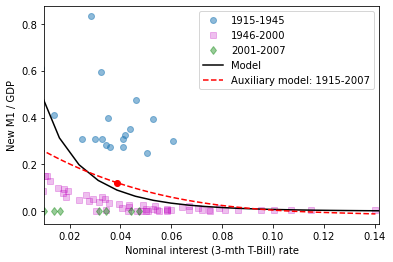
\includegraphics[scale=0.6]{figures/moneydemand_new2}
\par\end{centering}
\caption{\citet{lucas-nicolini-2015-jme} money demand annual data (1915-2007),
model (green-dashed line) and auxiliary regression model target (red-dashed
line). The red dot refers to the sample average for nominal interest.\protect\label{fig:fit-money-demand}}
\end{figure}


\paragraph*{Hours worked: Identification and internal calibrations.}

The preference scaling parameter $\bar{U}_{DM}$, which determines
the relative size of DM and CM payoffs, is identified from empirically
measured hours worked. In the model, $\bar{U}_{DM}$ is related to
the marginal utility function $U_{1}$ via the individual money demand
and labor supply. (For details, see Equations \eqref{eq:CM=000020KKT=000020y-1}
and \eqref{eq:CM=000020equilibrium=000020labor=000020supply} in the
Online Appendix). Thus, $\bar{U}_{DM}$ influences individual optimal
labor supply. Through SME, $\bar{U}_{DM}$ is identified from average
labor hours, which is $0.33$ of total available hours per person
in the U.S. data.

It is worth noting that we do not target money or pricing distribution
statistics in our calibration. However, our benchmark calibration
implies an equilibrium price dispersion (standard deviation) statistic
of 21.7 percent. A study by \citet{kaplan-menzio2015-ier}, which
uses price-scanner data in the U.S., found that their big-data sample
of prices exhibits dispersion. Measured in terms of standard deviation,
price dispersion in the data ranges from 19 percent (if goods are
defined according to their universal product codes) to 36 percent
(if goods are aggregated with different name brands and sizes). A
generic-brand aggregation would imply a pricing distribution with
about 21 percent in terms of standard deviation.\footnote{We do not calibrate the model to match the empirical distribution
of consumers' money holdings. Our purpose in this paper is not to
build a full-fledged quantitative model. Since the SME with inflation
is not analytically tractable, we have to discipline the model by
calibration to some relevant statistics. Pursuing the matching of
statistics on pricing and money distributions may not be as relevant
at this stage given the lack of bells and whistles\textemdash \emph{i.e.},
additional exogenous shocks and (parametric) frictions\textemdash that
are usually employed in the empirical pursuits of large-scale, quantitative
heterogeneous-agent models. In this paper, the purpose is to take
an intermediate step to study how the mechanism of \citet{menzio-shi-sun2012-jet}\textemdash \emph{i.e.},
equilibrium agent behavior and distributions\textemdash responds under
alternative inflationary settings. This question remains unanalyzed
in the literature, and we need to do so before complicating the model
in a quantitative direction.}

\subsection{Calibrated SME: Equilibrium functions}

In Figure \ref{fig:Value-functions}, we plot the SME value functions
$\left(\tilde{V},\bar{V}\right)$ in the benchmark economy. In the
benchmark economy, our algorithm finds two lottery segments. We know
that the graph of $W\left(\cdot,\omega\right)$ is that of an affine
function. This is because the CM utility function is quasilinear,
so that $W$ is linear in $m$. The non-convex/concave value function
for DM buyers is $B\left(\cdot,\omega\right)$. We do not plot these
in the figure since the upper envelope of these two graphs give us
$\tilde{V}\left(\cdot,\omega\right)$, the thick solid green line
shown in the figure. (Note that due to relative scales, the lower
segment or the affine part of $\tilde{V}\left(\cdot,\omega\right)$
attributable to $W\left(\cdot,\omega\right)$ may appear ``flat''
in the figure but it is actually an increasing affine graph.) Denote
$\text{conv}\left\{ \cdot\right\} $ as the convex-hull set operator.
The solid magenta graph is the graph of $\bar{V}\left(\cdot,\omega\right)$
obtained through our convex-hull approximation scheme, once we have
located all the intersecting coordinates between the set $\text{graph}\left[\tilde{V}\left(\cdot,\omega\right)\right]$
and the upper envelope of the set $\text{conv}\left\{ \text{graph}\left[\tilde{V}\left(\cdot,\omega\right)\right],\left(0,0\right),\left(\bar{m},0\right)\right\} $.

\begin{figure}[H]
\begin{centering}
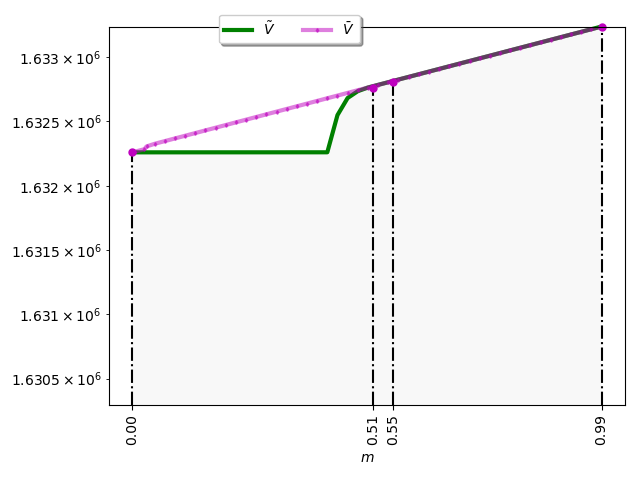
\includegraphics[width=0.5\textwidth]{figures/nbl/inflation-10/values}
\par\end{centering}
\caption{Value functions for benchmark economy.\protect\label{fig:Value-functions}}
\end{figure}

Sustaining the equilibrium value functions are the policy functions
$\left(l^{\star},b^{\star},x^{\star},q^{\star}\right)$, and the lottery
policies $\left(\pi_{1},1-\pi_{1}\right)$ and $\left(\pi'_{1},1-\pi'_{1}\right)$
over the prize supports $\left(z_{1},z_{2}\right)$ and $\left(z'_{1},z'_{2}\right)$,
where $\pi_{1}\left(m,\omega\right)=\left(z_{2}-m\right)/\left(z_{2}-z_{1}\right)$
and $\pi'_{1}\left(m,\omega\right)=\left(z'_{2}-m\right)/\left(z'_{2}-z'_{1}\right)$.

The other policy functions can be seen in Figure \vref{fig:Markov-policy-functions}.
Consider the panel depicting the graph of the CM labor supply function.
As shown in Proposition \ref{lem:CM=000020value=000020W=000020increasing,=000020concave,=000020continuous,=000020linear},
labor supply is affine and decreasing in money balance. There are
three shaded patches in the Figure's panels. The darker (and narrowest)
patch corresponds to the region where $m\in[0,k)$. In this region,
an agent will never match nor trade in the DM. The orange patches
(one of which overlaps the dark-red patch) are the regions of the
agent's state space in which a lottery may be played\textemdash i.e,
$\left[z_{1},z_{2}\right]$ and $\left[z'_{1},z'_{2}\right]$. What
matters for each agent in the SME is then the loci of these policy
functions outside of the orange patch, but including the points on
its boundary. These will be consistent with the equilibrium's ergodic
state space of agents. As shown in Proposition \ref{thm:=000020DM=000020value=000020and=000020policy=000020functions=000020in=000020SME},
the policy functions $\left(b^{\star},x^{\star},q^{\star}\right)$
are monotone in $m$ in the relevant subspace where an agent can exist
at any point in time. The relevant ergodic subspace of $\left[0,\bar{m}\right]$
in equilibrium is given by $\left\{ z_{1},\left[z_{2},z'_{1}\right],\left[z'_{2},\bar{m}\right]\right\} =\left\{ 0,\left[0.52,0.54\right],\left[0.98..,\bar{m}\right]\right\} $
in the benchmark economy in Figure \ref{fig:Value-functions} or Figure
\ref{fig:Markov-policy-functions}.

\begin{figure}[H]
\begin{centering}
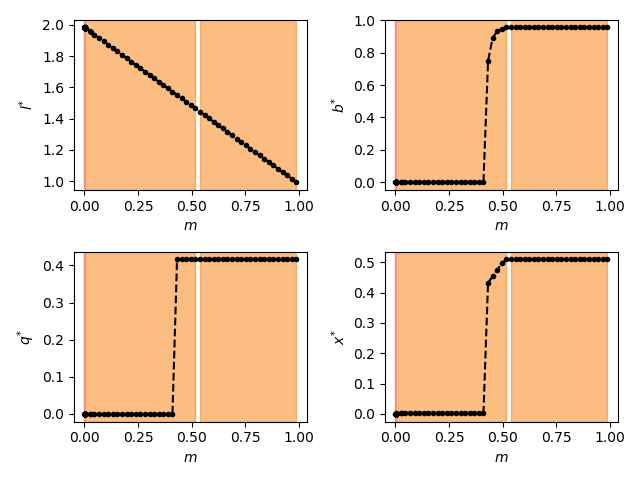
\includegraphics[width=0.8\textwidth]{figures/nbl/inflation-0/policies}
\par\end{centering}
\caption{\protect\label{fig:Markov-policy-functions}Markov policy functions
in the benchmark economy.}
\end{figure}
Given the information about our benchmark SME's active or relevant
agent state space and the corresponding policy functions, we can simulate
an agent's outcomes and also compute the equilibrium distribution
of real money holdings.\footnote{With competitive search, the domain of real money balances will be
finite. \citet{menzio-shi-sun2012-jet} derive a unique closed-form
for the graph of the distribution of money holdings, in the special
case of zero inflation. When there is non-zero inflation, this becomes
analytically intractable. We can numerically compute this, given agents'
equilibrium policy functions.} To do so, one may begin from any initial agent named $\left(m,\omega\right)$
and apply the decision rules computed earlier, as in Figure \ref{fig:Markov-policy-functions}.
Details of the algorithms for simulating the SME outcomes can be found
in our Online Appendix \ref{sec:Monte-Carlo-Simulation}. We now proceed
to discuss the equilibrium trade-offs faced by agents (\emph{i.e.},
the model mechanism) in the next section.

\section{Inflation, trade-offs and distribution\protect\label{subsec:Mechanism-tear-down}}

The results in our model are driven by a trade-off between the extensive
margin of trading probability and the intensive margin of trade quantities.
Consider the equilibrium description of firms' optimal DM production
in \eqref{eq:Q(x,b)}. Given the firms' best responses in a SME, a
potential DM buyer has the following trade-off: On one hand, faced
with a given probability $b$ of matching, the more a buyer is willing
to pay, $x$, the more $q$ she can consume. (This is the \emph{intensive
margin }of DM trade\textemdash \emph{i.e.}, how much one can purchase.)
On the other hand, given a required payment, $x,$ a buyer who seeks
to match with higher probability, $b$, tolerates consuming less $q$.
(This is the \emph{extensive margin }of DM trade\textemdash \emph{i.e.},
trading opportunities.)

In this section, we discuss \emph{how inflation affects individuals'
equilibrium intensive- and extensive-margin trade-offs} \emph{and
in turn impacts on money holdings and pric}es. The effects of inflation
on this well-known competitive search trade-off in heterogeneous-agent
models are not yet well-understood in the literature. This question
is what makes our adaptation of \citet{menzio-shi-sun2012-jet} to
an inflationary setting interesting and worthwhile of study.

In \citet{menzio-shi-sun2012-jet} and this model, when there is non-zero
inflation ($\tau\neq0$), agents' decision rules will depend on $\tau$
through the equilibrium, aggregate statistic $\omega$ (per-dollar
nominal wage). In turn, $\omega$ must be consistent with agents'
decisions through a market clearing requirement in a SME. However,
this also implies that there is no closed form characterization of
the equilibrium distribution of money, nor its expression as some
analytical function of $\tau$. Unlike the purely block-recursive
equilibrium feature under a zero-inflation setting in \citet{menzio-shi-sun2012-jet},
with inflation there is now only a partially block recursive SME \citep[see also a brief discussion in ][]{menzio-shi-sun2012-jet}.
We will develop our insights on the equilibrium behavior numerically,
by disciplining our analysis around the calibrated economy.\footnote{Partial block-recursivity under inflation also implies that we cannot
perform an analytical comparative-static analysis across different
$\tau$-induced SMEs. This is also the case in Bewley-Aiyagari types
of heterogeneous-agent models.}

Consider an increase in the long-run inflation rate from 0\% to 10\%
\emph{per annum}. We have the following observations regarding behavior
across the respective equilibria, denoted by SME$(\tau=0)$ and SME$(\tau=10)$.

\paragraph{CM labor supply (money demand) and inflation.}

First, we consider the effect of inflation on the intensive margin
of decision in the CM. This is summarized by the CM agents' labor
supply (which also implies money demand) response to inflation:

\begin{observation}
	Agents' optimal labor supply in the CM (demand for money) uniformly shifts down as inflation becomes higher. Average labor supply falls.
\end{observation}

\begin{figure}[H]
\begin{centering}
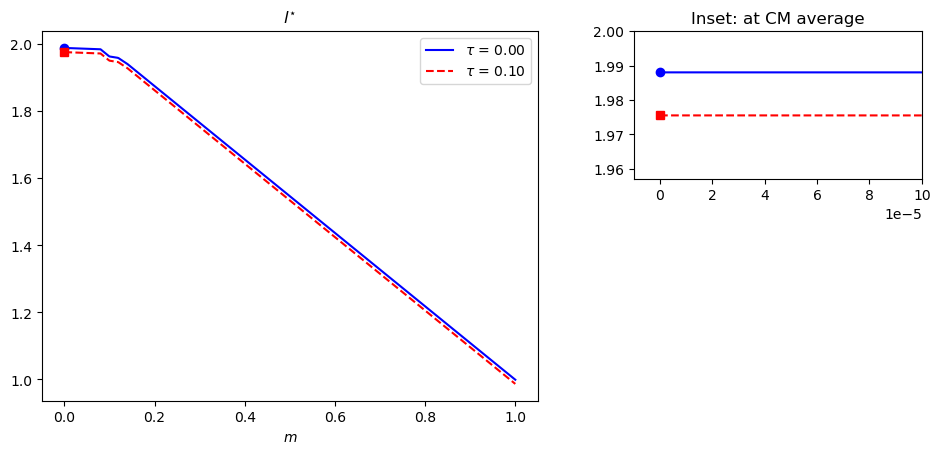
\includegraphics[width=0.55\textwidth]{figures/compare/mechanics/l-inflation}
\par\end{centering}
\caption{Labor supply falls with inflation. \emph{Notes}: For reference, the
circled-blue (squared-red) marker corresponds to the response of an
agent with an average money balance under SME$(\tau=0)$ (SME$(\tau=10)$).
Those who work turn out to be the agents who have zero initial money
balance. The inset figure zooms in to a subset of the graphs to emphasize
the relative positions of the averages.\protect\label{fig:l*=000020and=000020tau}}
\end{figure}

The solid-blue (dashed-red) graph in Figure \ref{fig:l*=000020and=000020tau}
depicts the SME labor supply as a function of $m$ when $\tau=0\%$
($\tau=10\%$) \emph{per annum. }For illustration, the circled-blue
and squared-red markers, respectively, correspond to the labor supply
responses of agents with an average money balance under SME$(\tau=0)$
and SME$(\tau=10)$. In both cases, the average is zero since the
agents who work in the CM are those with zero initial money balances.
The figure demonstrates that their labor supplies\textemdash and also
their money demands\textemdash fall with inflation. That is, with
higher inflation (tax) agents will tend to carry less money balances
over time.

\paragraph*{DM competitive-search extensive-intensive margins and inflation.}

Next we report the effects of inflation on the DM responses, where
the extensive margin arises.\begin{observation}
	As inflation becomes higher,  DM-buyers' optimal matching probability response shifts down. The elasticity of matching probability with respect to money balance falls uniformly.
\end{observation}

\begin{figure}[H]
\begin{centering}
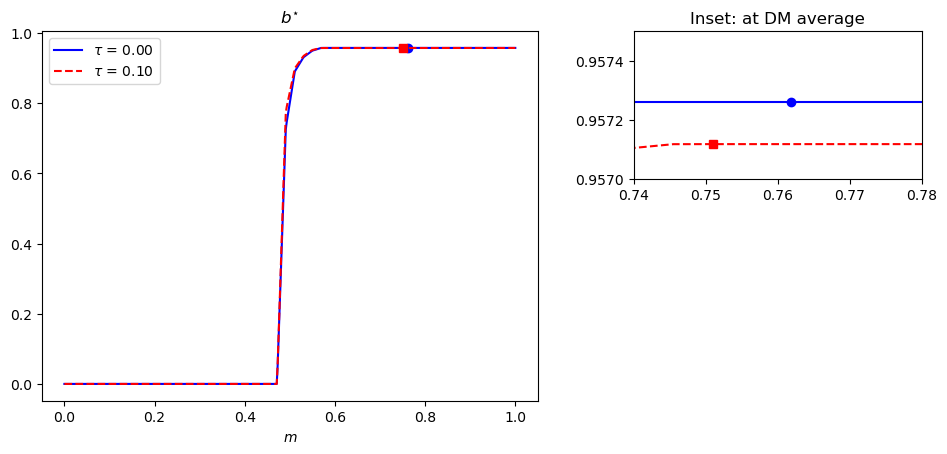
\includegraphics[width=0.6\textwidth]{figures/compare/mechanics/b-inflation}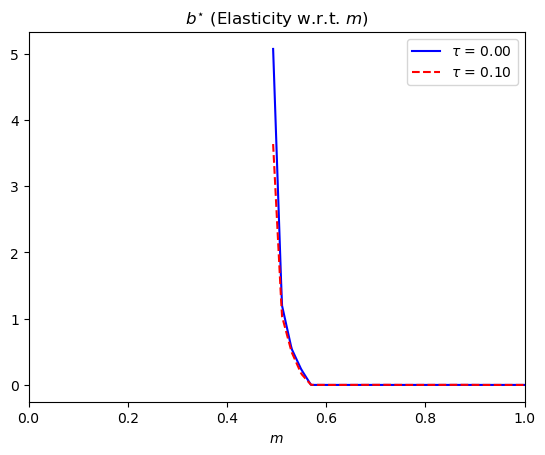
\includegraphics[width=0.35\textwidth]{figures/compare/mechanics/b-elasticity-inflation}
\par\end{centering}
\caption{DM-buyers' matching probability and its elasticity with respect to
money holdings shift down with higher inflation. \emph{Notes}: For
reference, the circled-blue (squared-red) marker corresponds to the
response of an agent with an average money balance under SME$(\tau=0)$
(SME$(\tau=10)$).\protect\label{fig:b*=000020and=000020tau}}
\end{figure}

In both main panels of Figure \ref{fig:b*=000020and=000020tau}, the
solid-blue graphs correspond to SME$(\tau=0)$ and the dashed-red
ones are for SME$(\tau=10)$. As in the previous figure, the circled-blue
and squared-red markers (with inset figure) correspond to the matching-probability
response of agents with an average money balance conditional on being
in the DM, under SME$(\tau=0)$ and SME$(\tau=10)$, respectively.
The uniform shift down in the matching probability function, in Figure
\ref{fig:b*=000020and=000020tau} (\emph{left panel}), is the \emph{extensive
margin} response to inflation: All else equal, higher inflation induces
agents in equilibrium to face lower matching rates with DM trading
posts. This margin, or force, also corresponds to a shift down in
agents' $m$-wealth elasticity of matching probabilities in Figure
\ref{fig:b*=000020and=000020tau} (\emph{right panel}). That is, these
agents would be optimally less $m$-wealth sensitive in their desired
matching rates.

Now consider the \emph{intensive margin }of competitive search:

\begin{observation}
	As inflation  becomes higher, DM-buyers' optimal payments uniformly shift down and average payment \emph{outcomes} fall.
\end{observation}

\begin{figure}[H]
\begin{centering}
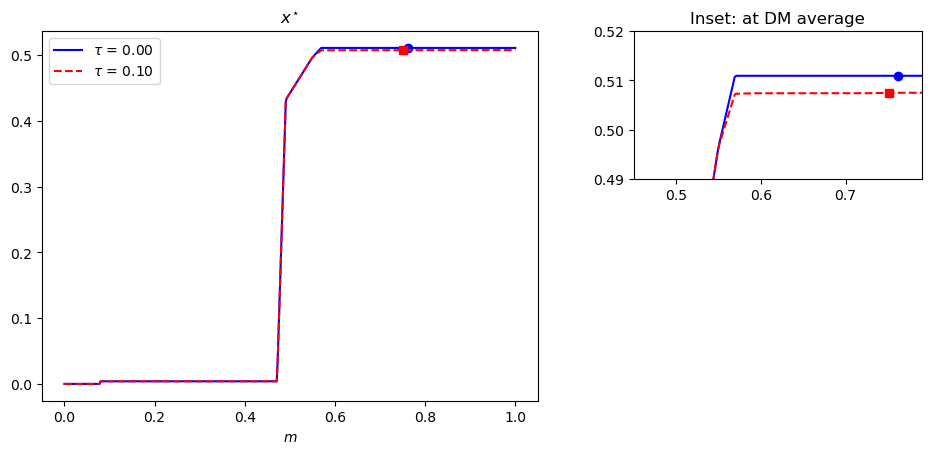
\includegraphics[width=0.55\textwidth]{figures/compare/mechanics/x-inflation}
\par\end{centering}
\caption{DM-buyers' payments schedule $x$ and inflation. \emph{Notes}: For
reference, the circled-blue (squared-red) marker corresponds to the
response of an agent with an average money balance under SME$(\tau=0)$
(SME$(\tau=10)$).\protect\label{fig:x=000020elasticity=000020and=000020tau}}
\end{figure}

However, from the previous observation, inflation also lowers money
holdings for agents entering each DM. This turns out to be particularly
the case for the average DM agents. The average DM agent ends up with
an \emph{outcome} of matching at a lower probability, offering less
payment, and this corresponds to a less elastic matching probability
with respect to money balance.

Consider the firms' side of the DM. In Figure \ref{fig:p=000020response=000020and=000020tau}
we compute the pricing function implied from the equilibrium behavioral
functions for DM total payments in submarkets ($x$) and traded goods
($q$)\textemdash \emph{i.e.}, $p:=x/q$. Higher inflation causes
the function $p$ to uniformly shift up.

\begin{figure}[H]
\begin{centering}
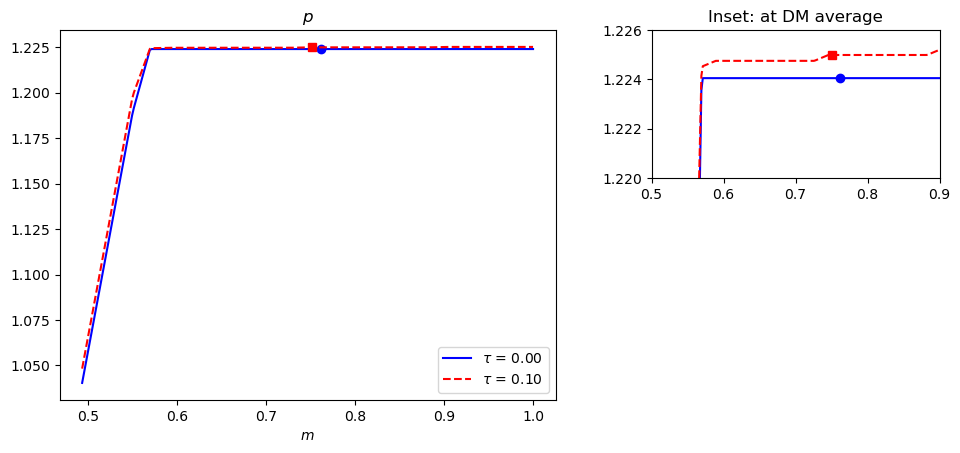
\includegraphics[width=0.55\textwidth]{figures/compare/mechanics/p-inflation}
\par\end{centering}
\caption{DM (submarkets) pricing function ($p$) and inflation. \protect\label{fig:p=000020response=000020and=000020tau}}
\end{figure}


\paragraph*{DM speed of trading and CM liquidity-management participation.}

The last discussion is also connected to how fast agents expect to
spend their monies in the DM. This will be tied to how often they
re-enter the CM to manage their liquidity positions. To see this,
we illustrate the implied expected transactions per dollar, $b\circ x/m$,
under each inflationary equilbrium, SME$(\tau=0)$ and SME$(\tau=10)$.

\begin{observation}
Agents trade faster: Individual per-dollar expenditure, $bx/m$, rises with inflation on average. High money balance agents are less sensitive in their speed of trading with respect to their money balance  than low money balance agents.
\end{observation}

Although $b$ and $x$ uniformly fall with inflation (see the previous
observation), each agent optimally would have a per-dollar expected
expenditure response function $b\circ x/m$ that may rise or fall
with inflation. This is shown in Figure \ref{fig:bxm=000020and=000020tau}
(\emph{left panel}). However, on average they expect to be ``trading
faster'' and offloading their money balance each time they expect
to trade in the DM. Moreover, Figure \ref{fig:bxm=000020and=000020tau}
(\emph{right panel}) shows that high-$m$ agents are also less sensitive
in their speed of trading with respect to $m$ than low-$m$ agents.
\begin{figure}[H]
\begin{centering}
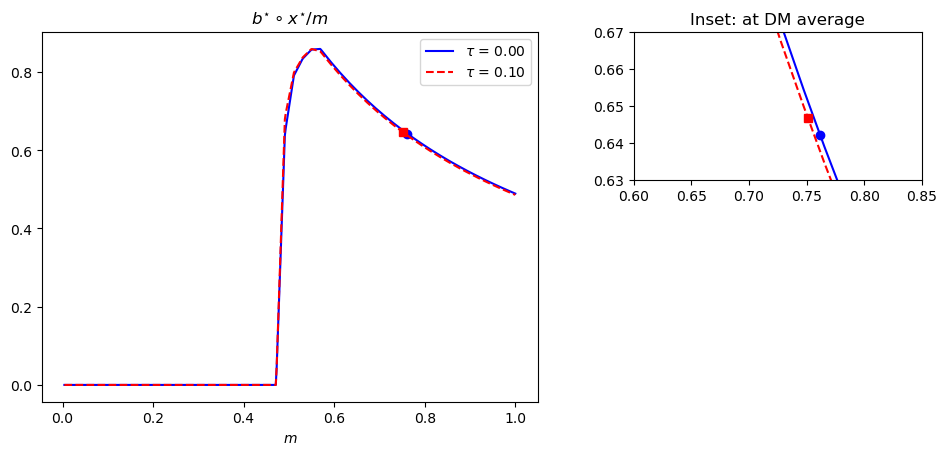
\includegraphics[width=0.55\textwidth]{figures/compare/mechanics/bxm-inflation}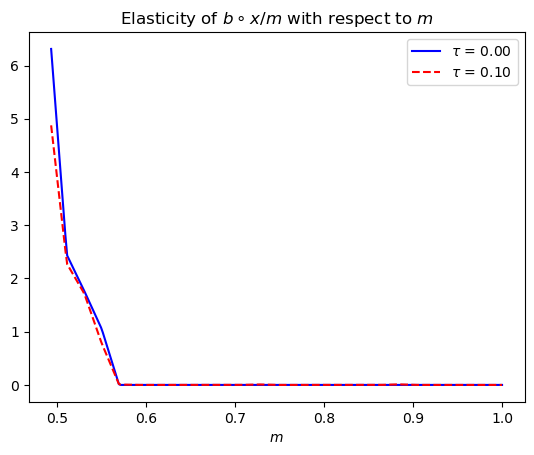
\includegraphics[width=0.3\textwidth]{figures/compare/mechanics/bxm-elasticity-inflation}
\par\end{centering}
\caption{DM-buyers' (implied) expected transactions per dollar, $b\circ x/m$,
and inflation. \emph{Notes}: For reference, the circled-blue (squared-red)
marker corresponds to the response or elasticity of an agent with
an average money balance under SME$(\tau=0)$ (SME$(\tau=10)$).\protect\label{fig:bxm=000020and=000020tau}}
\end{figure}

The equilibrium best responses above suggest to us a few key insights
about agents at different money positions: At a given inflation rate,
the higher money-balance (``rich'') agents are less elastic with
respect to money balance in terms of their matching probabilities
and velocities of spending in the DM. With higher inflation, although
average outcomes of DM buyer matching rates and payments become lower,
the average outcome of DM speed of transactions become higher. (This
finding is further reinforced by the observation that the top-10\%
of DM agents trade faster relative to the bottom-10\% as inflation
rise. See Figure \ref{fig:Agents-trade-faster}.)

\paragraph*{Intensive-extensive margin: Distributional effects of inflation.}

The previous discussion centers on equilibrium decision or allocation
functions, as well as the responses of the average money-balance agents,
conditional on them being in the CM or DM. We now consider agents
across the entire distribution of money holding. In addition, instead
of illustrating comparative equilibria using an equilibrium with 0\%
inflation and one with 10\% inflation \emph{per annum}, we now consider
a set of economies ordered by different inflation at (just above)
the Friedman rule to 10\% \emph{per }annum\emph{.}

We now use the calibrated model to demonstrate how the\emph{ }intensive-versus-extensive-margin
tension resolves, in the face of higher inflation. On the horizontal
axes of the following figures, we increase the (quarterly) steady-state
inflation rate, $\tau$, within the set $\left(\beta-1,0.025\right]$.
On the vertical axes, we measure relevant statistics for each corresponding
economy under policy $\tau$.

We begin with the distribution of agents in the DM (or the DM-conditional
distribution of agents) since fundamental source of the trade-off
arises in the DM. We shall see that the pattern induced by inflation
on the distributions of outcomes here will also emerge in the aggregate
distribution of agents' money holdings.

In Figure \ref{fig:Buyer-matching-probabilities-quantities-1} (\emph{top
left and right panel}s), the dashed and circled lines denote the bottom-
and the top-ten percent of outcomes, of the respective SME($\tau$)
distributions (conditional on agents in the DM), at each inflation
rate. The ``rich'' face a slower decline in their total payments
($x^{\star}$) for DM goods relative to the ``poor'', with respect
to higher inflation (Figure \ref{fig:Buyer-matching-probabilities-quantities-1}
(\emph{top-left} \emph{panel})). Also, while matching probabilities
of all buyers fall with inflation, the ``rich'' experience a slower
decline in these probabilities relative to the ``poor'' (see Figure
\ref{fig:Buyer-matching-probabilities-quantities-1} (\emph{bottom
panel})). Therefore, there is an increased dispersion in total payments
and trading probabilities.

\begin{figure}[tbh]
\begin{centering}
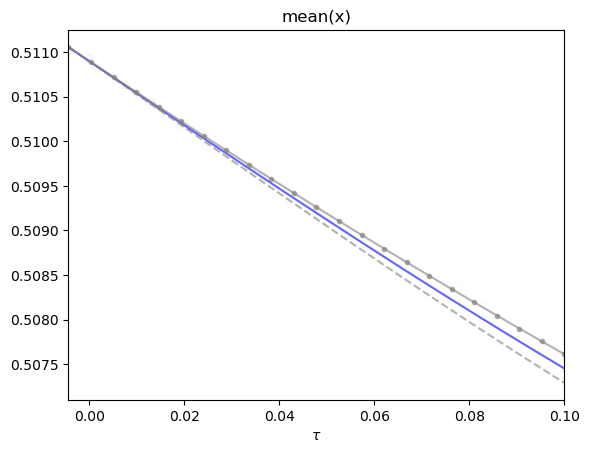
\includegraphics[width=6cm]{figures/compare2021/x} 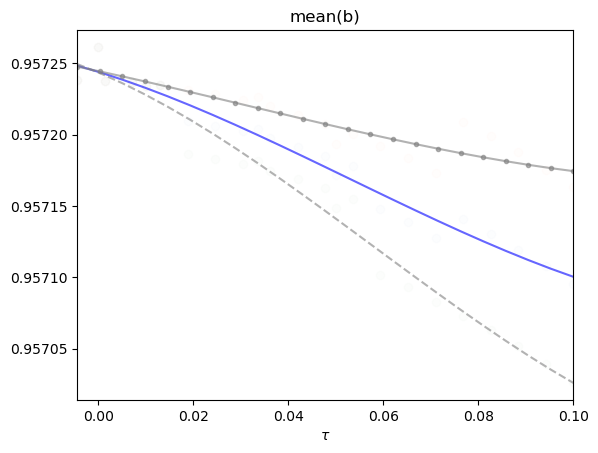
\includegraphics[width=6cm]{figures/compare2021/b}
\par\end{centering}
\begin{centering}
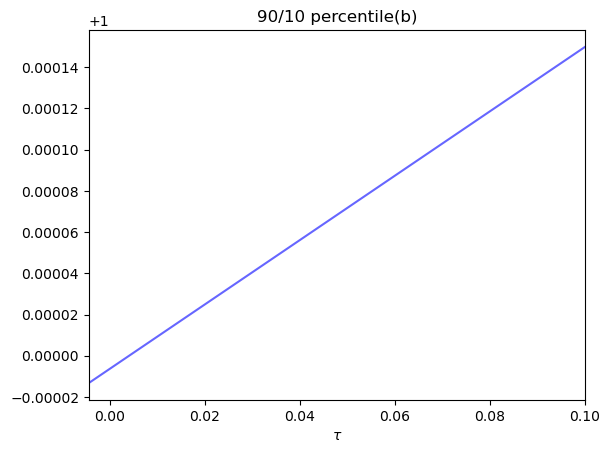
\includegraphics[width=6cm]{figures/compare2021/inequality-b-9010}
\par\end{centering}
\caption{Buyer matching probabilities and quantities\textemdash Mean (top panels,
solid), 90\% (solid-dotted) and 10\% (dashed) percentiles of DM-conditional
distribution of agents.\protect\label{fig:Buyer-matching-probabilities-quantities-1}}
\end{figure}
\begin{observation}
On average, agents end up paying less and matching at lower rates as inflation becomes higher. However, the decline of these outcomes with inflation is flatter for the ``rich'' agents than the ``poor'' agents. This induces the distribution of payments and matching risk in the DM to widen or be more dispersed.
\end{observation}

\textcolor{black}{Another way to see the increased dominance of the
extensive or trading-opportunity margin as inflation rises is as follows.
Consider Figure \ref{fig:Agents-trade-faster}. Since the probability
of not getting matched, $1-b^{\star}\left(m\right)$, increases with
inflation for all agents in the DM, this exacerbates the cost of holding
money for DM buyers who are unmatched, especially those holding higher
money balances. We observe that across the distribution of agents,
matching probabilities $b^{\star}\left(m\right)$ decrease with inflation.
However, what matters for DM agents is how quickly they can dispose
of a given amount of liquidity they carry into each DM round to exchange
for DM goods. Above, we introduced a useful summary statistic: the
(average) payment in the DM across buyers, $bx$/$m$. This ratio
increases with inflation. This means that within the DM-conditional
distribution, the dispersions in matching rates, payments, and transaction
velocities increase with inflation, with the ``rich'' agents facing
a less steep decline in these outcomes than the ``poor'' agents.
This symptom is the consequence of what we outlined above regarding
the dominance of the DM extensive margin as inflation rises.}

\begin{figure}[tbh]
\begin{centering}
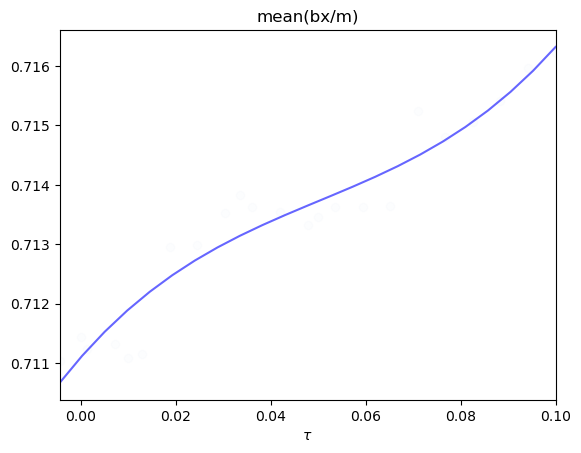
\includegraphics[width=6cm]{figures/compare2021/bxm}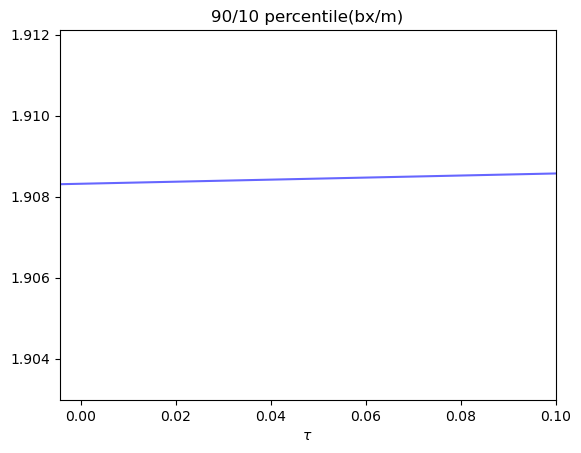
\includegraphics[width=6cm]{figures/compare2021/inequality-bxm-9010}
\par\end{centering}
\begin{centering}
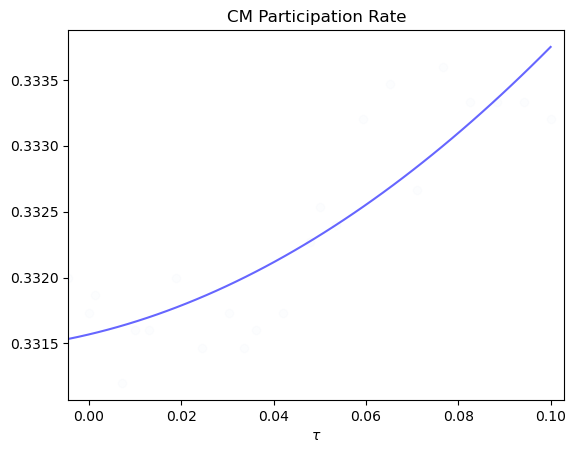
\includegraphics[width=6cm]{figures/compare2021/CMpart}
\par\end{centering}
\caption{\emph{Top-left}: On average, agents expect to have a higher per-dollar
spending rate in the DM, \emph{i.e.}, to \textquotedblleft trade faster\textquotedblright .
\emph{Top-right: }Inflation tends to make the rich trade faster than
the poor\textemdash the dispersion (90/10 ratio) in expected DM spending
per-dollar rises with inflation. \emph{Bottom}:\emph{ }Agents trade
faster on average in DM and return to CM quicker. \protect\label{fig:Agents-trade-faster}}
\end{figure}

At the distributional level, we again see the intensive-versus-extensive-margins
tension through Figure \ref{fig:Agents-trade-faster} (\emph{top-right
panel}): as inflation rises, their average spending per dollar rises
faster relative to the ``poor''. A consequence of this is that agents
would also go to the CM more often to manage their liquidity, as shown
in Figure \ref{fig:Agents-trade-faster} (\emph{bottom panel}). We
summarize what we have thus far:

\begin{observation}
On average, agents expect to have a higher per-dollar spending rate in the DM, i.e., to ``trade faster''. The rich agents trade faster on average in the DM and return to the CM quicker as inflation rises.
\end{observation}

\textcolor{black}{In summary, the extensive margin effect creates
more dispersion in the matching, payment and speed-of-trading outcomes
in the DM. This tends to work against the redistributive or compression
effect of inflation. For low inflation, the latter dominates and for
higher inflation, the former takes over. Figure \ref{fig:Inflation-and-money-distribution-DM}
shows the effect of this tension on the DM-conditional distribution
of money, across inflation regimes. We summarize this in the following
observation:}

\begin{figure}[th]
\begin{centering}
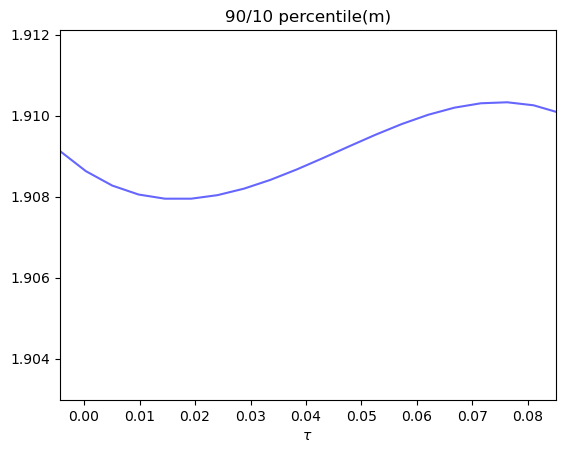
\includegraphics[width=7cm]{figures/compare2021/inequality-m-9010}
\par\end{centering}
\caption{Inflation and DM-conditional money distributions' inequality statistic
(ratio of 90-th to 10th percentile).\protect\label{fig:Inflation-and-money-distribution-DM}}
\end{figure}

\begin{observation}
At low inflation rates there is non-monotonicity in the inequality (90/10 percentile-ratio) of money balances of DM agents as a function of inflation.
\end{observation}

\paragraph*{\textcolor{black}{Overall money and pricing distributions and inflation.}}

\textcolor{black}{We next show that the non-monotone inequality effect
of inflation in the DM gets inherited in the overall (DM-and-CM) distribution
of money and prices.}

\textcolor{black}{Figure \ref{fig:Inflation-and-money-distribution}
reports an alternative Gini measure for money holdings inequality
for the overall distribution.}\footnote{We use the Gini measure here since the overall distribution contains
agents in the CM, and quantitatively, there are at least 10\% of agents
that hold zero money balances. (See Online Appendix \ref{sec:Inflation-and-overall-distro}
for two examples of the overall distribution.) As such, the 90/10
ratio is not well defined. Using the Gini measure also further reinforces
the point that the U-shaped inequality feature from the DM gets inherited
in the overall distribution of agents. We thank an anonymous referee
for clarifying this detail.

We also note that we have experimented with arbitrarily high inflation
beyond 10\textbackslash\% per annum. In such cases, the dispersion
in money wealth will begin to fall as the economy tends towards a
non-monetary equilibrium. At some point, the SME will break down:
One would expect that as monetary equilibrium should disappear with
hyperinflation. However, that is not the focus of this paper.} The green square marker in Figure \ref{fig:Inflation-and-money-distribution}
(\emph{bottom panel}) denotes a reference SME at zero inflation, or
at $\tau=0$. The red diamond marker is at an SME with annual inflation
of 10\%.

\begin{figure}[th]
\begin{centering}
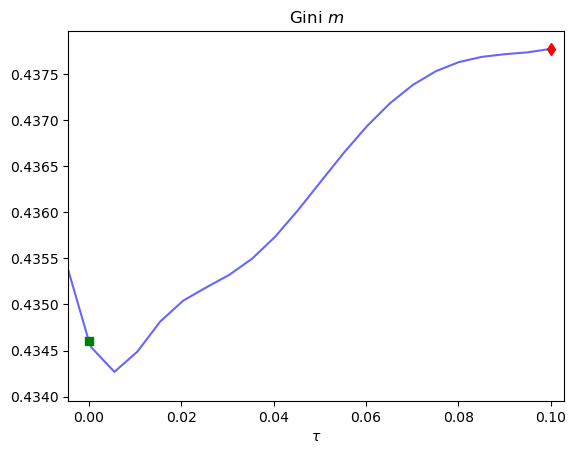
\includegraphics[width=6cm]{figures/compare2021/gini-m}
\par\end{centering}
\caption{Inflation and the Gini coefficient for the overall money distribution.\protect\label{fig:Inflation-and-money-distribution}}
\end{figure}

Finally, a feature of competitive search in this \citet{menzio-shi-sun2012-jet}-type
model is that there is potentially an equilibrium-determined dispersion
in goods' terms-of-trade or pricing outcomes. This provides further
motivation to study the effect of inflation in this \citet{menzio-shi-sun2012-jet}
type of monetary, heterogeneous-agent model where agents are free
to choose their participation in markets, which gives rise to endogenous
trading opportunities. As illustrated in Figure \ref{fig:Inflation-and-price},
both the average price and price dispersion increase with each inflationary
equilibrium.

\begin{figure}[H]
\begin{centering}
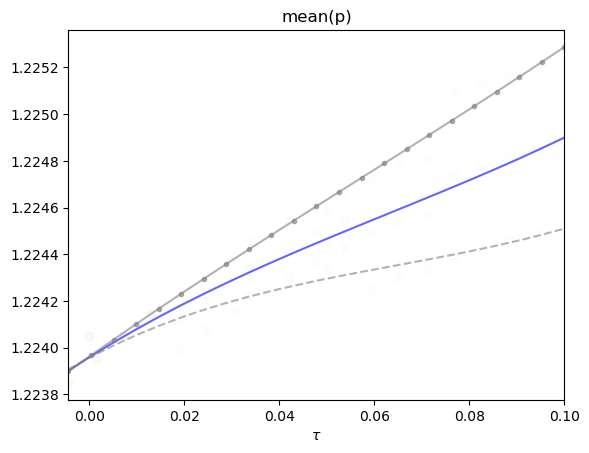
\includegraphics[width=6cm]{figures/compare2021/p}
\par\end{centering}
\caption{Inflation and price dispersion. Mean (solid), 90\% (solid-dotted)
and 10\% (dashed) percentiles of prices.\protect\label{fig:Inflation-and-price}}
\end{figure}

\begin{observation}
There is also a non-monotone inequality (Gini index) in money balances of all agents as a function of inflation. 
Prices increase and price dispersion rises with inflation.
\end{observation}

In summary, the extensive margin of search is an additional conduit
for inflation to impact on the cross section of money holdings by
affecting their heterogeneous matching probabilties. Unlike the results
in earlier heterogeneous-agent monetary models \citep[see, e.g.,][]{imhoroglu-prescott1991-jmcb,erosa-ventura-2002-jme},
inflation may not necessarily be a redistributive tax that reduces
(money) wealth inequality. With a trade-off between inflation tax
on the intensive margin of allocations and inflation incentivizing
agents to trade faster on the extensive margin, we get non-monotone
distributional consequences\textemdash a U-shaped inflation-money-inequality
relationship.

\section{Inflation and welfare\protect\label{sec:Inflation-and-welfare}}

We now turn to the traditional question of the welfare cost of inflation,
from the calibrated model's perspective. We measure welfare as how
much consumption equivalent variation (CEV) an ex-ante agent is willing
to give up in order to move from a zero-inflation economy to a higher-inflation
one. This CEV measure falls with inflation.\footnote{An individual's \emph{ex-ante} welfare is naturally measured as $Z_{\tau}:=\int\bar{V}\left(m,\omega\left(\tau\right)\right)\text{d}G(m,\omega(\tau))$.
Consider a reference equilibrium, SME$\left(\tau_{0}\right)$. Its
corresponding individuals' \emph{ex-ante} value is $Z_{\tau_{0}}$.
In an alternative economy SME$\left(\tau\right)$, the consumption
equivalent variation (CEV) required to move the individual from the
reference $\tau_{0}$-economy to the $\tau$-economy will be defined
as
\[
CEV\left(\tau\right)=\left[\frac{U^{-1}\left(Z_{\tau}\right)}{U^{-1}\left(Z_{\tau_{0}}\right)}-1\right]\times100\%.
\]
This individual-specific variation is measured in units of the CM
good (\emph{i.e.}, labor). In the comparisons, we set $\tau_{0}=0$,
\emph{i.e.}, the zero-inflation economy.}

\begin{figure}[tbh]
\begin{centering}
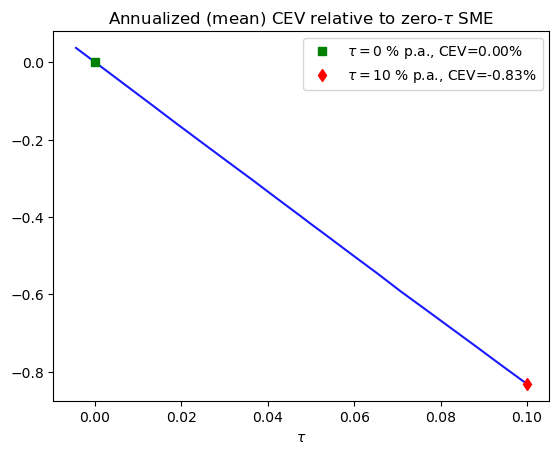
\includegraphics[width=6cm]{figures/compare2021/cev_mean}
\par\end{centering}
\caption{Mean welfare (CEV) falls for all types (0\% to 10\% inflation \emph{p.a.}).\protect\label{fig:Welfare-(CEV)-distribution}}
\end{figure}

Figure \ref{fig:Welfare-(CEV)-distribution} shows that the welfare
cost of inflation rises with inflation, for both average agents and
other agents across the respective distributions. Consider the solid
line in Figure \ref{fig:Welfare-(CEV)-distribution}: The\emph{ mean}
welfare cost of moving the economy from zero (green-square marker)
to ten percent (red-diamond marker) inflation \emph{per annum} is
about 0.83 percent of consumption loss (relative to the zero-inflation
SME mean consumption outcome.

\paragraph*{Cross-model welfare cost comparisons.}

In Table \ref{tab:Welfare-cost-(CEV)-comparison-models}, we compare
our model's welfare cost of inflation with some well-known studies
in the literature. In representative-agent models such as \citet{lucas2000-ecta}
and \citet{lagos-wright2005-jpe} (which has additional bargaining
frictions), the comparative-steady-state welfare cost of inflation
can be quite high. However, this welfare cost tends to be lower when
one revisits the question in a heterogeneous-agent version of the
models. It is well known that the redistributive margin of inflation
tax is always present in heterogeneous-agent models. This margin tends
to reduce the inefficiency of holding money in the presence of inflation
\citep[see, e.g.,][]{chien-camera-2014-jmcb,kocherlakota2005-ier,erosa-ventura-2002-jme}.
This is also the case in random-matching versions of such models \citep[see, e.g.,][]{chiu-molico2010-jme,molico2006-ier}.
In contrast, in heterogeneous-agent models such as \citet{imhoroglu-prescott1991-jmcb},
with more free parameters to govern frictions, one could obtain a
welfare cost of inflation as high as 0.9 percent \emph{per annum}
in CEV terms.

\begin{table}[H]
\begin{center}
\begin{threeparttable}
\begin{small}

\caption{Welfare cost (CEV) from 0\% to 10\% (p.a.) inflation economy.\protect\label{tab:Welfare-cost-(CEV)-comparison-models}}

\begin{centering}
\begin{tabular}{lcc}
\toprule 
\textbf{Economy} & \textbf{Welfare Cost} (\%)$^{a}$ & \textbf{Remarks}\tabularnewline
\midrule
Benchmark & $\boldsymbol{0.83}$ / $\boldsymbol{1.31}$ & static / transition\tabularnewline
Imhoro\u{g}lu-Prescott (1991)\nocite{imhoroglu-prescott1991-jmcb} & $0.90$ & Bewley-CIA$^{b}$-HA$^{d}$\tabularnewline
Chiu-Molico (2010)\nocite{chiu-molico2010-jme} & $0.41$ & RM$^{c}$-HA$^{d}$\tabularnewline
Lagos-Wright (2005)\nocite{lagos-wright2005-jpe} & $1.32$ & RM$^{c}$-RA$^{e}$-TIOLI$^{f}$\tabularnewline
Lucas (2000)\nocite{lucas2000-ecta} & $0.87$ & CIA$^{b}$-RA$^{e}$\tabularnewline
\bottomrule
\end{tabular}
\par\end{centering}
\begin{tablenotes}
	\item[a] Annualized CEV cost (relative to zero-inflation economy)
	\item[b] CIA: Cash-in-advance model
	\item[c] RM: Random matching model
	\item[d] HA: Heterogeneous agent model
	\item[e] RA: Representative agent model
	\item[f] TIOLI: Take-it-or-leave-it bargaining
\end{tablenotes}

\end{small}
\end{threeparttable}
\end{center}
\end{table}
We also calculate the (mean) welfare cost of inflation between a zero-inflation
and a ten-percent-inflation SME, taking into account the effects of
\emph{transitional dynamics}. Figure \ref{fig:Transition-from-zero-to-ten}
shows the transition of the aggregate state variable in terms of total
money holdings (\emph{left panel}) and its inverse statistic which
is the model's real wage rate, $\omega$ (\emph{right panel}). The
vertical axes are measure in percentage deviations from the respective
outcomes in the new or terminal SME. The economy is assumed to be
in the initial SME($\tau$) where money supply growth rate is $\tau_{-1}=0$
percent. At date $t=-1$, money supply growth rate jumps to $\tau_{-1}^{\prime}=\tau^{\prime}=10$
percent\emph{ per annum. }The economy reacts in date $t=0$ and takes
some time to transit to the new SME($\tau^{\prime}$). We use a standard
shooting algorithm to compute the transition. Total welfare cost of
inflation, along the transition is 1.31 percent of the initial SME's
consumption, as summarized in Table \ref{tab:Welfare-cost-(CEV)-comparison-models}
for our benchmark economy.

\begin{figure}
\begin{centering}
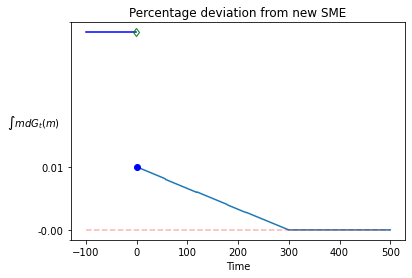
\includegraphics[width=6cm]{figures/compare2021/transition-m} 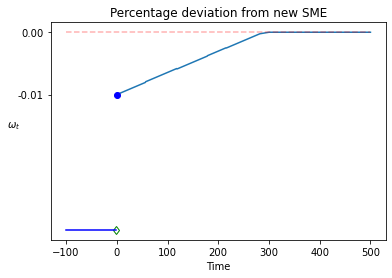
\includegraphics[width=6cm]{figures/compare2021/transition-omega}
\par\end{centering}
\caption{Transition from zero- to ten-percent-inflation SME. \emph{Left}: Aggregate
money. \emph{Right}: Real wage rate.\protect\label{fig:Transition-from-zero-to-ten}}
\end{figure}


\section{Conclusion\protect\label{sec:Conclusion}}

How inflation drives trading-probability and spending intensity trade-off
of individuals in heterogeneous-agent search models remained an open
question. In such a setting due to \citet*{menzio-shi-sun2012-jet},
we study the effect of long-run inflation on welfare and money-holdings
inequality.

We show that the endogenous trade-off between these intensive and
extensive margins culminate in a non-monotone effect of inflation
on money-holdings inequality. The effect of inflation tax on liquid-wealth
inequality is also non-monotone. Thus, the welfare cost of inflation
in our model is sizable, despite the redistributive effect of inflation
that tends to induce heterogenous-agent monetary models to produce
lower costs of inflation, relative to their representative-agent counterparts.

In this paper, we focus on a single-asset, pure-currency economy in
order to have a simple and clear understanding of the the effect of
inflation on equilibrium extensive- and intensive-margins of trade-off
of individuals and its distributional consequence. We think that if
we allowed agents to hold additional illiquid assets (say, in the
centralized markets), this may further exarcerbate the inequality
result in our model. We are currently exploring this conjecture in
an expanded setting with liquid and illiquid assets, and, further
with aggregate dynamics.\footnote{Since the framework renders agents' Markov decision processes independent
from the aggregate distribution, but for an aggregate scalar statistic,
we will have an exact \citet{krusell-smith1998-jpe} sort of algorithm
for computing equilibria. This is especially pertinent for the extended
setting with aggregate dynamics, as the competitive search refinement
means that the solution method can be made more efficient and more
precise, than models where one has to brute-force approximate distributions
when solving agent problems.}

%\begin{small}
\begin{spacing}{0.5}
\relsize{-1}

\bibliographystyle{aer}
\bibliography{references}

\end{spacing}
%\end{small}

\pagebreak{}

%%%%%%%% APPENDICES %%%%%%%%%%%%%%%%%%%%%%%%%%%%%%%%%%%%%%%%%%%%%%%% 
\newpage 
\thispagestyle{empty} 	
\begin{center} 		
	{\Huge\scshape\bfseries Online Appendix} 
	\bigskip

	{\Large{Inflation, Inequality, and Welfare in a Competitive Search Heterogeneous-agent Model}}



	\vfill
	
		\emph{Omitted Proofs and Other Results}
\\

This document is also available from
\\

\url{https://github.com/phantomachine/csm}.
	
\end{center}

\vspace{2cm}

	{Timothy Kam, \texttt{tcy.kam@gmail.com}}

    {Tina Kao, \texttt{tina.kao@anu.edu.au}}

	{Junsang Lee, \texttt{junsang.skku@gmail.com}}

\setcounter{page}{1} 	
\pagenumbering{arabic} 
\renewcommand\thepage{OA.\thesection-\arabic{page}}

\appendix

\vspace{2cm}
\newpage

\section{Extension and special cases\protect\label{sec:An-extension-and-special=000020cases}}

Consider a variation on the benchmark setting in the paper. In particular,
suppose that each agent $\mathbf{s}:=(m,\omega)$ has an initial value
each period as
\begin{equation}
\bar{V}\left(\mathbf{s}\right)=\alpha W\left(\mathbf{s}\right)+\left(1-\alpha\right)V\left(\mathbf{s}\right),\label{eq:Vbar=000020definition}
\end{equation}
where $V(\mathbf{s})$ is the value of playing a fair lottery $\left(\pi_{1},1-\pi_{1}\right)$
over the prizes $\left\{ z_{1},z_{2}\right\} $, \emph{i.e.},

\begin{equation}
V(\mathbf{s})=\max_{\pi_{1}\in[0,1],z_{1},z_{2}}\left\{ \pi_{1}\tilde{V}(z_{1},\omega)+\left(1-\pi_{1}\right)\tilde{V}\left(z_{2},\omega\right):\pi_{1}z_{1}+(1-\pi_{1})z_{2}=m\right\} ;\label{eq:Ex=000020ante=000020value-1}
\end{equation}
 is a natural upper bound on CM saving (in real money balances).

The difference between \eqref{eq:Vbar=000020definition} and \eqref{eq:Ex=000020ante=000020value-1}
and their respective counterparts in \eqref{eq:Ex=000020ante=000020value}
and \eqref{eq:Ex=000020ante=000020value-binary=000020choice} in Section
\vref{subsec:Ex-ante-decision} of the paper, is that there is a measure
$\alpha$ of agents who will participate in the CM for sure each period.

We have the following cases:
\begin{enumerate}
\item When $\alpha=0$, we recover the model presented in the main paper.
\item When $\alpha=0$, $U\left(C\right)=0$ for all $C$, and the labor
utility function $h(l)$ is strictly convex, we recover the original
\citet{menzio-shi-sun2012-jet} model as a special case.
\item Note that when $\alpha=1$ (\emph{i.e.}, agents get to enter the CM
deterministically), and the continuation value from CM is a convexification
of $B(\cdot,\omega)$, our model becomes a version of \citet{rocheteau-wright-2005-ecta}
with competitive search markets without agent and price dispersion.
\end{enumerate}
All proofs (to results in the paper) below are written with the more
general case of $\alpha\in[0,1)$ in mind.

\section{CM individual's problem\protect\label{sec:CM-individual's-problem}}

\paragraph{Preliminaries.}

Consider the feasible choice set for CM saving, $y$: If $\bar{m}$
is an upper bound on end-of-period balance plus transfer (measured
in units of labor), then this gives the bounds on end-of-period money
balance plus transfer, in current money value, as:
\[
\tau M\leq\omega My+\tau M\leq\omega M\bar{m},
\]
where $\omega M$ is current nominal wage. Since there is inflation
in nominal wage, then next-period initial balance is current end-of-period
nominal money balance normalized by the next period nominal wage $M_{+1}\omega_{+1}$,
\emph{i.e.},
\[
\frac{\tau M}{\omega_{+1}M_{+1}}\leq m_{+1}\equiv\frac{\omega My+\tau M}{\omega_{+1}M_{+1}}\leq\frac{\omega M\bar{m}}{\omega_{+1}M_{+1}}.
\]
Using \eqref{eq:money=000020growth}, we can re-write the above bounds
as
\[
0\leq y\leq y_{\text{max}}\left(\omega;\tau\right):=\bar{m}-\frac{\tau}{\omega},
\]
which applies in the pair of KKT complementary slackness conditions
\vref{eq:CM=000020KKT=000020y-1}.

The upper bound on real, end-of-period money holdings, $\bar{m}\in\left(0,\infty\right)$,
can be derived as:
\begin{equation}
0<\bar{m}<\left(U_{1}\right)^{-1}(1)\iff1<U_{1}(\bar{m})<U_{1}(0).\label{eq:Assumption-bounds=000020on=000020l=000020and=000020m}
\end{equation}

Later, in Part 3 of this section, we show that in any equilibrium
$U'(C)=1$. Assuming $U'(C)=1<U_{1}(\bar{m})$ suffices. Intuitively,
this permits an agent to accumulate real balances at the end of each
period beyond the level of optimal CM consumption $C^{\star}=U'{}^{-1}(1)$.
Below, we show that having $\bar{m}\in\left(0,\infty\right)$ will
ensure that there is always an optimal, largest labor effort that
is always finite and that in all dates, money balances are bounded.

The following gives the proof of Proposition \vref{lem:CM=000020value=000020W=000020increasing,=000020concave,=000020continuous,=000020linear}
in the paper.
\begin{center}
\begin{minipage}[t]{0.95\textwidth}%
\begin{shaded}%
\begin{prop}
\label{lem:CM=000020value=000020W=000020increasing,=000020concave,=000020continuous,=000020linear}Assume
$\tau/\omega<\bar{m}$. For a given sequence of prices $\left\{ \omega,\omega_{+1},...\right\} $,
the value function of the individual beginning in the CM, $W\left(\cdot,\omega\right)$,
has the following properties:
\begin{enumerate}
\item \textit{\label{enu:CM=000020W=000020Lemma-part1-1}$W\left(\cdot,\omega\right)\in\mathcal{V}[0,\bar{m}]$,
}\textit{\emph{i.e.}}\textit{, it is continuous, increasing and concave
on $\left[0,\bar{m}\right]$. Moreover, it is linear on $\left[0,\bar{m}\right]$.}
\item \textit{\label{enu:CM=000020W=000020Lemma-part2-1}The partial derivative
functions $W_{1}\left(\cdot,\omega\right)$ and $\bar{V}_{1}\left(\cdot,\omega_{+1}\right)$
exist and satisfy the first-order condition
\begin{equation}
\frac{\beta}{1+\tau}\left(\frac{\omega}{\omega_{+1}}\right)\bar{V}_{1}\left(\frac{\omega y^{\star}\left(m,\omega\right)+\tau}{\omega_{+1}\left(1+\tau\right)},\omega_{+1}\right)\begin{cases}
\leq1, & y^{\star}\left(m,\omega\right)\geq0\\
\geq1, & y^{\star}\left(m,\omega\right)\leq y_{\text{max}}\left(\omega;\tau\right)
\end{cases},\label{eq:CM=000020KKT=000020y-1}
\end{equation}
and the envelope condition:
\begin{equation}
W_{1}\left(m,\omega\right)=1,\label{eq:CM=000020Envelop=000020Condition-1}
\end{equation}
where $y^{\star}(m,\omega)=m+l^{\star}(m,\omega)-C^{\star}(m,\omega)$,
$l^{\star}(m,\omega)$ and $C^{\star}(m,\omega)$, respectively, are
the associated optimal choices of labor effort and consumption in
the CM.}
\item \textit{\label{enu:CM=000020policies=000020unique,=000020continuous,=000020monotone-1}The
stationary Markovian policy rules $y^{\star}\left(\cdot,\omega\right)$
and $l^{\star}\left(\cdot,\omega\right)$ are scalar-valued and continuous
functions on $\left[0,\bar{m}\right]$.}
\begin{enumerate}
\item \textit{The function $y^{\star}\left(\cdot,\omega\right)$ is constant
valued on $\left[0,\bar{m}\right]$.}
\item \textit{The optimizer $l^{\star}\left(\cdot,\omega\right)$ is an
affine and decreasing function on $\left[0,\bar{m}\right]$.}
\item \textit{Moreover, for every $\left(m,\omega\right)$, the optimal
choice $l^{\star}(m,\omega)$ is interior: $0<l_{\min}\leq l^{\star}\left(m\right)\leq l_{\max}\left(\omega;\tau\right)<+\infty$,
where there is a very small $l_{\text{min}}>0$ and $l_{max}\left(\omega\right):=y_{\text{max}}\left(\omega;\tau\right)+U^{-1}\left(1\right)<2U^{-1}\left(1\right)\in\left(0,\infty\right)$.}
\end{enumerate}
\end{enumerate}
\end{prop}
\end{shaded}%
\end{minipage}
\par\end{center}

{} % ad hoc spacer
\begin{proof}
(\emph{Part }\ref{enu:CM=000020W=000020Lemma-part1-1}). Consider
the individual's problem beginning in the CM \eqref{eq:CM=000020Bellman}.
Since $U_{1}\left(C\right)>0$ for all $C$, the budget constraint
always binds. Thus we can re-write \eqref{eq:CM=000020Bellman} as
\begin{multline}
W(\mathbf{s})=\max_{\left(C,y\right)\in\mathbb{R}_{+}\times\left[0,\bar{m}\right]}\biggl\{ U(C)-\left[pC+y-m\right]+\beta\bar{V}\left(\frac{\omega y+\tau}{\omega_{+1}\left(1+\tau\right)},\omega_{+1}\right)\biggr\}.\label{eq:CM=000020Bellman-1}
\end{multline}
Let
\begin{equation}
\left(C^{\star},y_{c}^{\star}\right)\left(m,\omega\right)\in\underset{\left(C,y\right)\in\mathbb{R}_{+}\times\left[0,\bar{m}\right]}{\arg\max}\left\{ U(C)-\left[pC+y-m\right]+\beta\bar{V}\left(\frac{\omega y+\tau}{\omega_{+1}\left(1+\tau\right)},\omega_{+1}\right)\right\} .\label{eq:CM=000020Bellman-1=000020optimizers}
\end{equation}
From \eqref{eq:CM=000020Bellman-1}, it is clear that $W_{1}\left(\cdot,\omega\right)$
exists on $\left[0,\bar{m}\right]$, and moreover, we have the envelope
condition $W_{1}\left(\cdot,\omega\right)=1>0$. This implies that
the value function $W\left(\cdot,\omega\right)$ is continuous, increasing
and concave in $m$. Moreover it is affine in $m$.

(\emph{Part }\ref{enu:CM=000020W=000020Lemma-part2-1}). First, we
make the following observations: Since $U$ is strictly concave in
$C$, the objective function is strictly concave in $C$. Moreover,
the objective function on the RHS of \eqref{eq:CM=000020Bellman-1}
is continuously differentiable with respect to $C$. The optimal decision,
$C^{\star}\left(m,\omega\right)$ satisfies the following Karush-Kuhn-Tucker
(KKT) conditions:
\begin{equation}
U_{1}\left(C\right)\begin{cases}
=p, & C>0\\
<p, & C=0
\end{cases}.\label{eq:CM=000020KKT=000020c}
\end{equation}
In an equilibrium, $p>0$ will be finite\textemdash in fact, $p=1$.
Therefore, $C^{\star}\left(m,\omega\right)\equiv\bar{C}^{\star}=\left(U_{1}\right)^{-1}\left(1\right)$
is a finite and non-negative constant. Thus, we only have to verify
that the optimal decision correspondence, given by $l_{c}^{\star}\left(m,\omega\right)\equiv p\bar{C}^{\star}+y_{c}^{\star}\left(m,\omega\right)-m$
at each $\left(m,\omega\right)$, exists and is at least a compact-valued
and upper-semicontinuous (\emph{usc}) correspondence: Fixing $C=\bar{C}^{\star}$,
the objective function on the RHS of \eqref{eq:CM=000020Bellman-1}
is continuous and concave on the compact choice set $\left[0,\bar{m}\right]\ni y$.
By Berge's Maximum Theorem, the maximizer $y_{c}^{\star}\left(m,\omega\right)$,
or $l_{c}^{\star}\left(m,\omega\right)$, is compact-valued and \emph{usc}
on $\left[0,\bar{m}\right]$. (After we further establish that the
derivative $V_{1}\left(\cdot,\omega_{+1}\right)$ exists, we show
below that it is constant and single-valued with respect to $m$.)

Second, we take a detour and show that the derivative $\bar{V}_{1}\left(\cdot,\omega_{+1}\right)$
exists. This will be used later to characterize a first-order condition
with the respect to $y$. The results below relies on the observation
that since $V$$\left(\cdot,\omega_{+1}\right)$ is a concave, real-valued
function on $\left[0,\bar{m}\right]$, it has right- and left-hand
derivatives \citep[see, e.g.,][Theorem 24.1, pp.227-228]{rockafellar1970}.
Fix $C^{\star}\left(m,\omega\right)\equiv\bar{C}^{\star}$. Since
$y_{c}^{\star}\left(m,\omega\right)$ is \emph{usc} on $\left[0,\bar{m}\right]$,
then for all $\varepsilon\in\left[0,\delta\right]$, and taking $\delta\searrow0$,
there exists a selection $y^{\star}\left(m-\varepsilon,\omega\right)\in y_{c}^{\star}\left(m-\varepsilon,\omega\right)$
feasible to a CM agent $m$. Similarly, there is a $y^{\star}\left(m,\omega\right)\in y_{c}^{\star}\left(m,\omega\right)$
that is feasible to a CM agent $m-\varepsilon$. Moreover, if $l^{\star}\left(m,\omega\right)\in l_{c}^{\star}\left(m,\omega\right)$
is an optimal selection associated with $y^{\star}\left(m,\omega\right)$,
then for an agent at $m$,
\begin{multline*}
W\left(m,\omega\right)=\underset{\equiv Z\left[m,y^{\star}\left(m,\omega\right)\right]}{\underbrace{U\left(\bar{C}^{\star}\right)-l^{\star}\left(m,\omega\right)+\beta\bar{V}\left[\frac{\omega\left[m+l^{\star}\left(m,\omega\right)-\bar{C}^{\star}\right]+\tau}{\omega_{+1}\left(1+\tau\right)},\omega_{+1}\right]}}\\
\geq\underset{\equiv Z\left[m,y^{\star}\left(m-\varepsilon,\omega\right)\right]}{\underbrace{U\left(\bar{C}^{\star}\right)-l^{\star}\left(m-\varepsilon,\omega\right)+\beta\bar{V}\left[\frac{\omega\left[m+l^{\star}\left(m-\varepsilon,\omega\right)-\bar{C}^{\star}\right]+\tau}{\omega_{+1}\left(1+\tau\right)},\omega_{+1}\right]}};
\end{multline*}
and, for an agent at $m-\varepsilon$,
\begin{multline*}
W\left(m-\varepsilon,\omega\right)\\
=\underset{\equiv Z\left[m-\varepsilon,y^{\star}\left(m-\varepsilon,\omega\right)\right]}{\underbrace{U\left(\bar{C}^{\star}\right)-l^{\star}\left(m-\varepsilon,\omega\right)+\beta\bar{V}\left[\frac{\omega\left[\left(m-\varepsilon\right)+l^{\star}\left(m-\varepsilon,\omega\right)-\bar{C}^{\star}\right]+\tau}{\omega_{+1}\left(1+\tau\right)},\omega_{+1}\right]}}\\
\geq\underset{\equiv Z\left[m-\varepsilon,y^{\star}\left(m,\omega\right)\right]}{\underbrace{U\left(\bar{C}^{\star}\right)-l^{\star}\left(m,\omega\right)+\beta\bar{V}\left[\frac{\omega\left[\left(m-\varepsilon\right)+l^{\star}\left(m,\omega\right)-\bar{C}^{\star}\right]+\tau}{\omega_{+1}\left(1+\tau\right)},\omega_{+1}\right]}}.
\end{multline*}
Rearranging these inequalities, we have the following fact:
\begin{multline*}
\frac{Z\left[m,y^{\star}\left(m-\varepsilon,\omega\right)\right]-Z\left[m-\varepsilon,y^{\star}\left(m-\varepsilon,\omega\right)\right]}{m-\left(m-\varepsilon\right)}\\
\leq\frac{W\left(m,\omega\right)-W\left(m-\varepsilon,\omega\right)}{m-\left(m-\varepsilon\right)}\leq\frac{Z\left[m,y^{\star}\left(m,\omega\right)\right]-Z\left[m-\varepsilon,y^{\star}\left(m,\omega\right)\right]}{m-\left(m-\varepsilon\right)},
\end{multline*}
which, after simplifying the denominator and taking limits, yields:
\begin{gather*}
\lim_{\varepsilon\searrow0}\left\{ \frac{Z\left[m,y^{\star}\left(m-\varepsilon,\omega\right)\right]-Z\left[m-\varepsilon,y^{\star}\left(m-\varepsilon,\omega\right)\right]}{\varepsilon}\right\} \\
\leq\lim_{\varepsilon\searrow0}\left\{ \frac{W\left(m,\omega\right)-W\left(m-\varepsilon,\omega\right)}{\varepsilon}\right\} \leq\lim_{\varepsilon\searrow0}\left\{ \frac{Z\left[m,y^{\star}\left(m,\omega\right)\right]-Z\left[m-\varepsilon,y^{\star}\left(m,\omega\right)\right]}{\varepsilon}\right\} \\
\iff\\
\beta\lim_{\varepsilon\searrow0}\left\{ \frac{\bar{V}\left[\frac{\omega\left(m+l^{\star}\left(m-\varepsilon,\omega\right)-\bar{C}^{\star}\right)+\tau}{\omega_{+1}\left(1+\tau\right)},\omega_{+1}\right]-\bar{V}\left[\frac{\omega\left(m-\varepsilon+l^{\star}\left(m-\varepsilon,\omega\right)-\bar{C}^{\star}\right)+\tau}{\omega_{+1}\left(1+\tau\right)},\omega_{+1}\right]}{\varepsilon}\right\} \leq W_{1}\left(m,\omega\right)\\
\leq\beta\lim_{\varepsilon\searrow0}\left\{ \frac{\bar{V}\left[\frac{\omega\left(m+l^{\star}\left(m,\omega\right)-\bar{C}^{\star}\right)+\tau}{\omega_{+1}\left(1+\tau\right)},\omega_{+1}\right]-\bar{V}\left[\frac{\omega\left(m-\varepsilon+l^{\star}\left(m,\omega\right)-\bar{C}^{\star}\right)+\tau}{\omega_{+1}\left(1+\tau\right)},\omega_{+1}\right]}{\varepsilon}\right\} .
\end{gather*}
Since, from \eqref{eq:CM=000020Bellman-1}, $W\left(\cdot,\omega\right)$
is clearly differentiable with respect to $m$, the second term in
the inequalities above is equal to the partial derivative $W_{1}\left(m,\omega\right)$,
which is constant. As $\varepsilon\searrow0$, there is a selection
$l^{\star}\left(m-\varepsilon,\omega\right)\rightarrow l^{\star}\left(m,\omega\right)$,
and, by \citet[Theorem 24.1]{rockafellar1970} the first is the left
derivative of $\bar{V}\left(\cdot,\omega_{+1}\right)$. Moreover,
the last term is identical to the first, \emph{i.e.},
\begin{multline*}
\frac{\beta}{1+\tau}\left(\frac{\omega}{\omega_{+1}}\right)\bar{V}_{1}\left[\frac{\omega\left(m^{-}+l^{\star}\left(m,\omega\right)-\bar{C}^{\star}\right)+\tau}{\omega_{+1}\left(1+\tau\right)},\omega_{+1}\right]\\
\leq W_{1}\left(m,\omega\right)\leq\frac{\beta}{1+\tau}\left(\frac{\omega}{\omega_{+1}}\right)\bar{V}_{1}\left[\frac{\omega\left(m^{-}+l^{\star}\left(m,\omega\right)-\bar{C}^{\star}\right)+\tau}{\omega_{+1}\left(1+\tau\right)},\omega_{+1}\right].
\end{multline*}
Therefore, if the optimal selection is interior, these weak inequalities
must hold with equality, so we have the left derivative of $\bar{V}$
with respect to the agent's decision variable $y$ as:
\[
\frac{\beta}{1+\tau}\left(\frac{\omega}{\omega_{+1}}\right)\bar{V}_{1}\left[\frac{\omega y^{\star-}\left(m,\omega\right)+\tau}{\omega_{+1}\left(1+\tau\right)},\omega_{+1}\right]=W_{1}\left(m,\omega\right).
\]
where $y^{\star-}\left(m,\omega\right)\equiv m^{-}+l^{\star}\left(m,\omega\right)-\bar{C}^{\star}$.

By similar arguments, we can also prove that the right directional
derivative of $\bar{V}\left(\cdot,\omega_{+1}\right)$ exists, and
show that the right derivative of $\bar{V}$ with respect to the agents
decision $y$ as:
\[
\frac{\beta}{1+\tau}\left(\frac{\omega}{\omega_{+1}}\right)\bar{V}_{1}\left[\frac{\omega y^{\star+}\left(m,\omega\right)+\tau}{\omega_{+1}\left(1+\tau\right)},\omega_{+1}\right]=W_{1}\left(m,\omega\right),
\]
where $y^{\star+}\left(m,\omega\right)\equiv m^{+}+l^{\star}\left(m,\omega\right)-\bar{C}^{\star}$.
From the last two equations, we can conclude that the right and left
directional derivatives must agree, and thus, we have the first-order
KKT condition as
\[
\frac{\beta}{1+\tau}\left(\frac{\omega}{\omega_{+1}}\right)\bar{V}_{1}\left(\frac{\omega y^{\star}\left(m,\omega\right)+\tau}{\omega_{+1}\left(1+\tau\right)},\omega_{+1}\right)\begin{cases}
\leq1, & y^{\star}\left(m,\omega\right)\geq0\\
\geq1, & y^{\star}\left(m,\omega\right)\leq y_{\max}\left(\omega;\tau\right)
\end{cases},
\]
where the weak inequalities apply with complementary slackness. Since
$\bar{V}$ is strictly concave, the condition above ensures a unique
selection $y^{\star}\left(m,\omega\right)$ at each state. Also, note
that in the previous proof of Part \ref{enu:CM=000020W=000020Lemma-part1-1}),
we have established the envelope condition:
\[
W_{1}\left(m,\omega\right)=1.
\]

(\emph{Part} \ref{enu:CM=000020policies=000020unique,=000020continuous,=000020monotone-1}\emph{.})
Observe that given the assumption in \eqref{eq:Assumption-bounds=000020on=000020l=000020and=000020m},
we have \eqref{eq:CM=000020KKT=000020c} always binding: $U'\left(C\right)=p=1$.
Also, observe from \eqref{eq:CM=000020KKT=000020c} and \eqref{eq:CM=000020KKT=000020y-1}
that an individual's current money holding $m$ and the aggregate
state $\omega$ have no influence on his optimal decision on consumption,
$C^{\star}\left(m,\omega\right)=\bar{C}^{\star}$. However, equilibrium
CM asset decision will depend on the aggregate state $\omega$, i.e.,
\begin{align}
y^{\star}\left(m,\omega\right) & =\bar{y}^{\star}\left(\omega\right)\label{CM=000020optimal=000020y*}
\end{align}
and this satisfies the first-order condition \eqref{eq:CM=000020KKT=000020y-1}.

However, from the budget constraint, $m$ clearly does affect the
optimal labor decision,
\begin{align}
l^{\star}(m,\omega) & =pC^{\star}\left(m,\omega\right)+y^{\star}\left(m,\omega\right)-m\nonumber \\
 & \underset{\left(p=1\right)}{\equiv}\bar{C}^{\star}+\bar{y}^{\star}\left(\omega\right)-m.\label{eq:CM=000020equilibrium=000020labor=000020supply}
\end{align}
Clearly, $l^{\star}(m,\omega)$ is single-valued, continuous, affine
and decreasing in $m$.

Finally, we show that the optimal choice of $l$ will always be interior.
Evaluating the budget constraint in terms of optimal choices at the
current individual state $m$,
\[
l^{\star}\left(m,\omega\right)=\bar{y}^{\star}\left(\omega\right)-m+\bar{C}^{\star}.
\]
Since $m\in\left[0,\bar{m}\right]$, then, the minimal $l$ attains
when $m$ is maximal at $\bar{m}$, and, $\bar{y}^{\star}\left(\bar{m},\omega\right)=0$:
\begin{align*}
l_{\min}: & =\check{l}^{\star}\left(\bar{m},\omega\right)\equiv0-\bar{m}+\bar{C}^{\star}>0.
\end{align*}
The last inequality obtains from \eqref{eq:Assumption-bounds=000020on=000020l=000020and=000020m}
which requires $\bar{m}<U^{-1}\left(1\right)$, and from optimal CM
consumption \eqref{eq:CM=000020optimal=000020C*} which yields
\begin{align}
C^{\star}\left(m,\omega\right) & \equiv\bar{C}^{\star}=\left(U_{1}\right)^{-1}\left(1\right),\label{eq:CM=000020optimal=000020C*}
\end{align}
a finite and non-negative constant.

The maximal $l$ attains when $m=0$ and $\bar{y}^{\star}\left(0,\omega\right)=y_{\text{max }}\left(\omega;\tau\right)$:
\begin{equation}
l_{\text{max}}\left(\omega,\tau\right):=y_{\text{max }}\left(\omega;\tau\right)-0+\bar{C}^{\star}=y_{\text{max}}\left(\omega;\tau\right)+U^{-1}\left(1\right)<2U^{-1}\left(1\right).\label{eq:lmax}
\end{equation}
Clearly, $l_{\text{max}}\left(\omega,\tau\right)<+\infty$. If we
do not have hyperinflation, or, if transfers are not excessively large\textemdash \emph{i.e.},
if $\tau/\omega<\bar{m}$\textemdash then, $l_{\text{max}}\left(\omega,\tau\right)>0$
will be well-defined. So if $\tau/\omega<\bar{m}$, then we will have
an interior optimizer for all $m$: $0<l_{\min}\leq l^{\star}\left(m\right)\leq l_{\text{max}}\left(\omega;\tau\right)<+\infty.$
\end{proof}

\section{DM agent's problem\protect\label{sec:DM-agent's-problem}}

In the main paper, we provided a verbal summary of the properties
of DM agents' equilibrium value function ($B$) and decision rules
($b,x,q$). Here we state these results precisely:
\begin{center}
\begin{minipage}[t]{0.88\textwidth}%
\begin{shaded}%
\begin{prop}[DM value and policy functions]
\label{thm:=000020DM=000020value=000020and=000020policy=000020functions=000020in=000020SME}
For a given sequence of prices $\left\{ \omega,\omega_{+1},...\right\} $,
the following properties hold.
\begin{enumerate}
\item \textit{For any $\bar{V}(\cdot,\omega_{+1})\in\mathcal{V}\left[0,\bar{m}\right]$,
the DM buyer's value function is increasing and continuous in money
balances, $B\left(\cdot,\omega\right)\in\mathcal{C}\left[0,\bar{m}\right]$.}
\item \textit{For any $m\leq k$, DM buyers' optimal decisions are $b^{\star}\left(m,\omega\right)=x^{\star}\left(m,\omega\right)=q^{\star}\left(m,\omega\right)=0$,
and $B\left(m,\omega\right)=\beta\bar{V}\left[\phi(m,\omega),\omega_{+1}\right]$,
where $\phi(m,\omega):=(\omega m+\tau)/\left[\omega_{+1}(1+\tau)\right]$.}
\item \textit{At any $\left(m,\omega\right)$, where $m\in\left[k,\bar{m}\right]$
and the buyer matching probability is positive $b^{\star}\left(m,\omega\right)>0$:}
\begin{enumerate}
\item \textit{The optimal selections $\left(x^{\star},b^{\star},q^{\star}\right)(m,\omega)$
and $\phi^{\star}(m,\omega):=\phi\left[m-x^{\star}\left(m,\omega\right),\omega\right]$,
are unique, continuous, and increasing in $m$.}
\item \textit{The buyer's marginal valuation of money $B_{1}(m,\omega)$
exists if and only if $\bar{V}_{1}\left[\phi(m,\omega),\omega\right]$
exists.}
\item \textit{$B(m,\omega)$ is strictly increasing in $m$.}
\item \textit{the optimal policy functions $b^{\star}$and $x^{\star}$,
respectively, satisfy the first-order conditions
\begin{multline}
u\circ Q\left[x^{\star}(m,\omega),b^{\star}(m,\omega)\right]+b^{\star}(m,\omega)\left(u\circ Q\right)_{2}\left[x^{\star}(m,\omega),b^{\star}(m,\omega)\right]\\
=\beta\left[\bar{V}\left(\phi\left(m,\omega\right),\omega_{+1}\right)-\bar{V}\left(\phi^{\star}\left(m,\omega\right),\omega_{+1}\right)\right],\label{eq:DM=000020FoC=000020w.r.t.=000020b}
\end{multline}
and,
\begin{equation}
\left(u\circ Q\right)_{1}\left[x^{\star}(m,\omega),b^{\star}(m,\omega)\right]=\frac{\beta}{1+\tau}\left(\frac{\omega}{\omega_{+1}}\right)\bar{V}_{1}\left[\phi^{\star}(m,\omega),\omega_{+1}\right].\label{eq:DM=000020FoC=000020w.r.t.=000020x}
\end{equation}
}
\end{enumerate}
\end{enumerate}
\end{prop}
\end{shaded}%
\end{minipage}
\par\end{center}

In the rest of this section, we prove the results leading up to Proposition
\vref{thm:=000020DM=000020value=000020and=000020policy=000020functions=000020in=000020SME}
in the paper. Part 1 of Proposition \vref{thm:=000020DM=000020value=000020and=000020policy=000020functions=000020in=000020SME}
is obtained in Lemma \ref{lem:DM=000020B=000020continuous,=000020increasing},
Part 2 is proven as Lemma \ref{lem:DM=000020B=000020no=000020trade=000020region}.
Part 3(a) is proven as Lemma \ref{lem:DM=000020policies=000020unique,=000020increasing,=000020continuous=000020at=000020m}.
Lemmata \ref{lemma:J'=00003Du'} and \ref{lem:DM=000020B=000020differentiable=000020a.e.}
together establish Parts 3(b) and 3(c) of Proposition \vref{thm:=000020DM=000020value=000020and=000020policy=000020functions=000020in=000020SME}.
Finally, Lemma \ref{lem:DM=000020FoCs} establishes Part 3(d) of Proposition
\vref{thm:=000020DM=000020value=000020and=000020policy=000020functions=000020in=000020SME}.

\subsection{DM buyer optimal policies}

Recall the DM buyer's problem from \eqref{eq:DM=000020Bellman=000020(x,b)}:
\[
B(\mathbf{s})=\max_{x\in[0,m],b\in[0,1]}\left\{ f\left(x,b;m,\omega\right)\right\} ,
\]
where
\begin{multline*}
f\left(x,b;m,\omega\right):=\beta(1-b)\left[\bar{V}\left(\frac{\omega m+\tau}{\omega_{+1}\left(1+\tau\right)},\omega_{+1}\right)\right]\\
+b\biggl[u^{Q}(x,b)+\beta\bar{V}\left(\frac{\omega\left(m-x\right)+\tau}{\omega_{+1}\left(1+\tau\right)},\omega_{+1}\right)\biggr],
\end{multline*}
and, we have re-defined the composite function $u\circ Q$ as $u^{Q}$.
Note that we have not explicitly written $f\left(x,b;m,\omega\right)$
as depending on $\omega_{+1}$ which is taken as parametric. In an
equilibrium, $\omega_{+1}$ will be recursively dependent on $\omega$,
thus our small sleight of hand here in writing $f\left(x,b;m,\omega\right)$.

The following Lemmata \ref{lem:DM=000020B=000020continuous,=000020increasing},
\ref{lem:DM=000020B=000020no=000020trade=000020region}, \ref{lem:DM=000020policies=000020unique,=000020increasing,=000020continuous=000020at=000020m},
\ref{lemma:J'=00003Du'}, \ref{lem:DM=000020B=000020differentiable=000020a.e.},
and \ref{lem:DM=000020FoCs} make up Proposition \ref{thm:=000020DM=000020value=000020and=000020policy=000020functions=000020in=000020SME}.
Also, these results will rely on the following statements and notations:
\begin{enumerate}
\item Assume $\left\{ \omega,\omega_{+1},\omega_{+2}...\right\} $ is a
given sequence of prices.
\item Let 
\begin{align*}
\phi(m,\omega): & =\frac{\omega m+\tau}{\omega_{+1}(1+\tau)},
\end{align*}
and, 
\[
\phi^{\star}(m,\omega)=\phi\left[m-x^{\star}(m,\omega),\omega\right].
\]
\item Equivalently define the objective function $f(\cdot,\cdot;m,\omega)$
in the DM buyer's problem \eqref{eq:DM=000020Bellman=000020(x,b)}
as follows:
\begin{align}
f\left(x,b;m,\omega\right) & =\beta\bar{V}\left(\frac{\omega m+\tau}{\omega_{+1}\left(1+\tau\right)},\omega_{+1}\right)\nonumber \\
 & +b\left[u^{Q}(x,b)+\beta\bar{V}\left(\phi^{\star}(m,\omega),\omega_{+1}\right)-\beta\bar{V}\left(\phi(m,\omega),\omega_{+1}\right)\right].\nonumber \\
 & \equiv\beta\bar{V}\left(\phi(m,\omega),\omega_{+1}\right)+bR\left(x,b;m,\omega\right).\label{eq:DM=000020objective}
\end{align}
\end{enumerate}
\begin{rem*}
Observe that maximizing the value of the objective function $f\left(x,b;m,\omega\right)$
in the DM buyer's problem \eqref{eq:DM=000020Bellman=000020(x,b)}
is equivalent to maximizing the second term, $bR\left(x,b;m,\omega\right)$.
Note that the function $R\left(x,b;m,\omega\right)$ has the interpretation
of the DM buyer's surplus from trading with a particular trading post
named $\left(x,b\right)$, by offering to pay $x$ in exchange for
quantity $Q(x,b)$.
\end{rem*}
{} %ad-hoc spacer

\begin{minipage}[t]{0.9\columnwidth}%
\begin{shaded}%
\begin{lem}
\label{lem:DM=000020B=000020continuous,=000020increasing}For any
$\bar{V}(\cdot,\omega_{+1})\in\mathcal{V}\left[0,\bar{m}\right]$,
the DM buyer's value function is increasing and continuous in money
balances, $B\left(\cdot;\omega\right)\in\mathcal{C}\left[0,\bar{m}\right]$.
\end{lem}
\end{shaded}%
\end{minipage}
\begin{proof}
Since the functions $W\left(\cdot,\omega_{+1}\right),V\left(\cdot,\omega_{+1}\right)\in\mathcal{C}\left[0,\bar{m}\right]$,
\emph{i.e.}, are continuous and increasing on $\left[0,\bar{m}\right]$,
and $\bar{V}:=\alpha W+\left(1-\alpha V\right)$, then $\bar{V}\left(\cdot,\omega_{+1}\right)\in\mathcal{C}\left[0,\bar{m}\right]$.
The feasible choice set $\Phi(m):=[0,m]\times[0,1]$ is compact, and
it expands with $m$ at each $m\in\left[0,\bar{m}\right]$. By Berge's
Maximum Theorem, the maximizing selections $\left(x^{\star},b^{\star}\right)\left(m,\omega\right)\in\Phi(m)$
exist for every fixed $m\in\left[0,\bar{m}\right]$, since the objective
function is continuous on a compact choice set \citep{berge-1959}.
Evaluating the Bellman operator \eqref{eq:DM=000020Bellman=000020(x,b)},
we have that the value function $B\left(\cdot,\omega\right)\in\mathcal{C}\left[0,\bar{m}\right]$.
\end{proof}
{} %ad-hoc spacer

\begin{minipage}[t]{0.9\columnwidth}%
\begin{shaded}%
\begin{lem}
\label{lem:DM=000020B=000020no=000020trade=000020region}For any $m\leq k$,
DM buyers' optimal decisions are such that $b^{\star}\left(m,\omega\right)=0$
and $B\left(m,\omega\right)=\beta\bar{V}\left[\phi(m,\omega),\omega_{+1}\right]$,
where $\phi(m,\omega):=\frac{\omega m+\tau}{\omega_{+1}(1+\tau)}$.
\end{lem}
\end{shaded}%
\end{minipage}
\begin{proof}
Since a buyer's payment $x$ is always constrained above by her initial
money balance $m$ in the DM, it will never be optimal for any firm
to trade with such a buyer whose $m\leq k$, as the firm will be making
an economic loss. In equilibrium it is thus optimal for a buyer $m\leq k$
to optimally not trade and exit the DM with end-of-period balance
as $m$ (\emph{i.e.}, with beginning-of-next-period balance $\phi(m,\omega)$
when inflationary transfers are accounted for). As a result, the continuation
value is $\bar{V}\left[\phi(m,\omega),\omega_{+1}\right]$, and thus,
$B\left(m,\omega\right)=\beta\bar{V}\left[\phi(m,\omega),\omega_{+1}\right]$,
if $m\leq k$.
\end{proof}
{} %ad-hoc spacer

\begin{minipage}[t]{0.9\columnwidth}%
\begin{shaded}%
\begin{lem}
\label{lem:DM=000020policies=000020unique,=000020increasing,=000020continuous=000020at=000020m}For
any $\left(m,\omega\right)$, where $m\in\left[k,\bar{m}\right]$
and the buyer matching probability is positive $b^{\star}\left(m,\omega\right)>0$,
the optimal selections $\left(x^{\star},b^{\star},q^{\star}\right)(m,\omega)$
and $\phi^{\star}(m,\omega):=\phi\left[m-x^{\star}\left(m,\omega\right),\omega\right]$
are unique, continuous, and increasing in $m$.
\end{lem}
\end{shaded}%
\end{minipage}

{}

\medskip %ad-hoc spacer

Observe that the DM buyer's problem has a general structure similar
to that of \citet{menzio-shi-sun2012-jet}. The main difference is
in the details underlying the buyer's continuation value function,
which in our setting is denoted by $\bar{V}\left(\cdot,\omega\right)$.
Nevertheless, we still have that $\bar{V}\left(\cdot,\omega\right)\in\mathcal{V}\left[0,\bar{m}\right]$.
As a consequence the proof of Lemma 3.3 in \citet{menzio-shi-sun2012-jet}
can be adapted to our setting. For the reader's convenience, we repeat
the proof strategy of \citet{menzio-shi-sun2012-jet} below for our
model setting in a few steps:
\begin{proof}
The DM buyer's problem \eqref{eq:DM=000020Bellman=000020(x,b)} can
be re-written as
\[
B(\mathbf{s})=\beta\bar{V}\left(\phi(m,\omega),\omega_{+1}\right)+\exp\left\{ \max_{x\in[0,m],b\in[0,1]}\left\{ \ln\left(b\right)+\ln\left[R\left(x,b;m,\omega\right)\right]\right\} \right\} .
\]
The optimizers thus must satisfy
\begin{equation}
(x^{\star},b^{\star})(m,\omega)\in\left\{ \arg\max_{x\in[0,m],b\in[0,1]}\left\{ \ln\left(b\right)+\ln\left[R\left(x,b;m,\omega,\omega_{+}\right)\right]\right\} \right\} .\label{eq:(x,b)=000020DM=000020optimum}
\end{equation}
(\emph{Uniqueness and continuity of policies}.) First we establish
that the policy functions are continuous, and, at every state, there
is a unique optimal selection: Since $u^{Q}\left(x,b\right)$ is continuous,
jointly and strictly concave in $(x,b)$, and by assumption, $\bar{V}\left(\cdot,\omega\right)\in\mathcal{V}\left[0,\bar{m}\right],$
then
\[
R\left(x,b;m,\omega\right)\equiv u^{Q}(x,b)+\beta\bar{V}\left(\phi^{\star}(m,\omega),\omega_{+1}\right)-\beta\bar{V}\left(\phi(m,\omega),\omega_{+1}\right)
\]
is continuous, jointly and strictly concave in the choice variables
$\left(x,b\right)$. Also, $\ln(b)$ is strictly increasing and strictly
concave in $b$. Thus the maximand is jointly and strictly concave
in $\left(x,b\right)$. By Berge's Maximum Theorem, the optimal selections
$(x^{\star},b^{\star})(m,\omega)$ are continuous and unique at any
$m$. Since $c\mapsto c(q)$ is bijective, then 
\begin{align*}
q^{\star}(m,\omega) & =c^{-1}\left[x^{\star}(m,\omega)-k/\mu\left(b^{\star}(m,\omega)\right)\right]
\end{align*}
 is continuous in $m$; and so is $\phi^{\star}(m,\omega).$

\medskip
%
\noindent(\emph{Monotonicity of policies.}) The remainder of this proof establishes
that the policy functions are increasing. The key idea of the proof
is in showing that the choice set is a lattice equipped with a partial
order, that the choice set is increasing in $m$, and, has increasing
differences on the choice set, and the slices of the buyer's objective
is supermodular in each given direction of his choice set. By Theorem
2.6.2 of \citet{topkis1998}, these properties are sufficient to ensure
that the buyer's objective function is supermodular. Together, these
properties suffice, by Theorem 2.8.1 of \citet{topkis1998}, for showing
that the buyer's optimal policies are increasing functions in $m$.
\begin{enumerate}
\item The function $R\left(\cdot,\cdot,\cdot,\omega\right)$ in \eqref{eq:(x,b)=000020DM=000020optimum}
has \emph{increasing difference }in $\left(x,b,m\right)$ and is therefore
supermodular:

Fix an $m\in\left[k,\bar{m}\right]$ and $b\in(0,1]$. (The case of
$b=0$ is trivially uninteresting.) It suffices to optimize over the
function $\ln\left[R\left(\cdot,b,m,\omega\right)\right]$ in \eqref{eq:(x,b)=000020DM=000020optimum}.
Then the optimizer
\[
\tilde{x}(b,m,\omega)\in\left\{ \arg\max_{x\in\left[k,\bar{m}\right]}\left\{ \ln\left[R\left(x,b,m,\omega\right)\right]\right\} \right\} 
\]
is unique for each $(m,b,\omega)$, since the objective functions
is strictly concave.

Next we show how the value of the objective function has increasing
differences in $\left(x,b,m\right)$, throughout taking the sequence
$\left\{ \omega,\omega_{+1},...\right\} $ as fixed. Thus we will
now write $R\left(x,b,m\right)\equiv R\left(x,b,m,\omega\right)$
to temporarily ease the notation. First, the feasible choice set 
\begin{align*}
\mathcal{F}_{m}: & =\left\{ \left(x,b,m\right):x\in\left[0,m\right],b\in\left[0,1\right],m\in\left[k,\bar{m}\right]\right\} ,
\end{align*}
 is a partially ordered set with relation $\leq$, and it has least-upper
and greatest-lower bounds. It is therefore a sublattice in $\mathbb{R}_{+}^{3}$.
Observe that $\mathcal{F}_{m}$ is increasing in $m$. Second, pick
any $m'>m$, $b'>b$, and $x'>x$ in $\mathcal{F}_{m}$:
\begin{enumerate}
\item \label{enu:id-a}Fix $x$, consider $m'>m$ and $b'>b$. Then, we
can write
\begin{multline*}
R\left(x,b',m'\right)-R\left(x,b,m\right)\\
\qquad=\left[u^{Q}(x,b')-u^{Q}(x,b)\right]\\
\qquad\qquad+\beta\left[\bar{V}\left(\frac{\omega\left(m'-x\right)+\tau}{\omega_{+1}\left(1+\tau\right)},\omega_{+1}\right)-\bar{V}\left(\frac{\omega\left(m-x\right)+\tau}{\omega_{+1}\left(1+\tau\right)},\omega_{+1}\right)\right]\\
-\beta\left[\bar{V}\left(\frac{\omega m'+\tau}{\omega_{+1}\left(1+\tau\right)},\omega_{+1}\right)-\bar{V}\left(\frac{\omega m+\tau}{\omega_{+1}\left(1+\tau\right)},\omega_{+1}\right)\right].
\end{multline*}
Observe that the RHS is separable in $b$ and $m$: The first term
on the right, $u^{Q}(x,b')-u^{Q}(x,b)<0$, shows increasing difference
in $b$. Likewise the remainder two difference terms on the RHS show
increasing differences in $m$. Overall $R\left(x,b,m\right)$ has
increasing differences on the lattice $\left[0,1\right]\times\left[0,\bar{m}\right]\ni\left(b,m\right)$.
\item \label{enu:id-b}Fix $m$, consider $x'>x$ and $b'>b$. Observe that
\begin{multline}
R\left(x,b,m\right)-R\left(x',b,m\right)=\left[u^{Q}(x,b)-u^{Q}(x',b)\right]\\
+\beta\left[\bar{V}\left(\frac{\omega\left(m-x\right)+\tau}{\omega_{+1}\left(1+\tau\right)},\omega_{+1}\right)-\bar{V}\left(\frac{\omega\left(m-x'\right)+\tau}{\omega_{+1}\left(1+\tau\right)},\omega_{+1}\right)\right].\label{eq:R=000020diff=000020x}
\end{multline}
Now, using the expression \eqref{eq:R=000020diff=000020x} twice below,
we have that
\begin{multline*}
\left[R\left(x',b',m\right)-R\left(x,b',m\right)\right]-\left[R\left(x',b,m\right)-R\left(x,b,m\right)\right]\\
=\left[u^{Q}(x',b')-u^{Q}(x,b')\right]\\
\qquad\qquad+\beta\left[\bar{V}\left(\frac{\omega\left(m-x'\right)+\tau}{\omega_{+1}\left(1+\tau\right)},\omega_{+1}\right)-\bar{V}\left(\frac{\omega\left(m-x\right)+\tau}{\omega_{+1}\left(1+\tau\right)},\omega_{+1}\right)\right]\\
\qquad\qquad-\left[u^{Q}(x',b)-u^{Q}(x,b)\right]\\
\qquad\qquad-\beta\left[\bar{V}\left(\frac{\omega\left(m-x'\right)+\tau}{\omega_{+1}\left(1+\tau\right)},\omega_{+1}\right)-\bar{V}\left(\frac{\omega\left(m-x\right)+\tau}{\omega_{+1}\left(1+\tau\right)},\omega_{+1}\right)\right]\\
=\left[u^{Q}(x',b')-u^{Q}(x,b')\right]-\left[u^{Q}(x',b)-u^{Q}(x,b)\right]>0,
\end{multline*}
where the last inequality is implied by the fact that $\left(u^{Q}\right)_{12}(x,b)>0$.
Therefore $R\left(x,b,m\right)$ has increasing differences on the
lattice $\left[0,m\right]\times\left[0,1\right]\ni\left(x,b\right)$.
\item \label{enu:id-c}For fixed $b$, consider $x'>x$ and $m'>m$. Observe
that
\begin{multline*}
\left[R\left(x',b,m'\right)-R\left(x,b,m'\right)\right]-\left[R\left(x',b,m\right)-R\left(x,b,m\right)\right]\\
=\left[u^{Q}(x',b)-u^{Q}(x,b)\right]\\
\qquad\qquad+\beta\left[\bar{V}\left(\frac{\omega\left(m'-x'\right)+\tau}{\omega_{+1}\left(1+\tau\right)},\omega_{+1}\right)-\bar{V}\left(\frac{\omega\left(m'-x\right)+\tau}{\omega_{+1}\left(1+\tau\right)},\omega_{+1}\right)\right]\\
\qquad\qquad-\left[u^{Q}(x',b)-u^{Q}(x,b)\right]\\
\qquad\qquad-\beta\left[\bar{V}\left(\frac{\omega\left(m-x'\right)+\tau}{\omega_{+1}\left(1+\tau\right)},\omega_{+1}\right)-\bar{V}\left(\frac{\omega\left(m-x\right)+\tau}{\omega_{+1}\left(1+\tau\right)},\omega_{+1}\right)\right]\\
=\beta\left[\bar{V}\left(\frac{\omega\left(m'-x'\right)+\tau}{\omega_{+1}\left(1+\tau\right)},\omega_{+1}\right)-\bar{V}\left(\frac{\omega\left(m'-x\right)+\tau}{\omega_{+1}\left(1+\tau\right)},\omega_{+1}\right)\right]\\
-\beta\left[\bar{V}\left(\frac{\omega\left(m-x'\right)+\tau}{\omega_{+1}\left(1+\tau\right)},\omega_{+1}\right)-\bar{V}\left(\frac{m-x+\tau}{1+\tau\omega},\omega_{+1}\right)\right]\geq0,
\end{multline*}
where the last weak inequality obtains from the property that $\bar{V}\left(\cdot,\omega_{+1}\right)\in\mathcal{V}\left[0,\bar{m}\right]$,
and $\bar{V}\left(\cdot,\omega_{+1}\right)$ is therefore weakly concave.
Therefore $R\left(x,b,m\right)$ has increasing differences on the
lattice $\left[0,m\right]\times\left[0,\bar{m}\right]\ni\left(x,m\right)$.
\end{enumerate}
From parts \eqref{enu:id-a}, \eqref{enu:id-b}, and \eqref{enu:id-c},
we can conclude that the objective function $R\left(\cdot,\cdot,\cdot,\omega\right)$
has increasing differences on $\mathcal{F}_{m}$. This suffices to
prove that the objective function $R\left(\cdot,\cdot,\cdot,\omega\right)$
is supermodular \citep[see][Corollary 2.6.1]{topkis1998}, since the
domain of the function is a direct product of a finite set of chains
(partially ordered sets with no unordered pair of elements), and the
objective function is real valued \citep[see][]{topkis1978-or}.
\item Since $R\left(\cdot,b,m\right)$ is supermodular, for fixed choice
$b$, the optimizer $\tilde{x}\left(b,m,\omega\right)$ is increasing
in $\left(b,m\right)$, for given $\omega$:

Let $\tilde{x}\left(b,m,\omega\right)=\arg\max_{x\in\left[0,m\right]}R\left(x,b,m\right)$.
From part \eqref{enu:id-a} above, we can deduce that for fixed $\tilde{x}\left(b,m\right)$,
$\tilde{R}\left(b,m\right)\equiv R\left[\tilde{x}\left(b,m,\omega\right),b,m\right]$
is supermodular on the lattice $\left[0,1\right]\times\left[0,\bar{m}\right]\ni\left(b,m\right)$.
Since $R(x,b,m)$ is strictly decreasing in $b$, then 
\begin{align*}
\tilde{R}\left(b,m\right) & \equiv R\left[\tilde{x}\left(b,m,\omega\right),b,m\right]
\end{align*}
is strictly decreasing in $b$. Observe that for any $m'\geq m$,
where $m',m\in\left[k,\bar{m}\right]$, we have
\begin{multline*}
R\left(x,b,m'\right)-R\left(x,b,m\right)\\
=\beta\left[\bar{V}\left(\frac{\omega m+\tau}{\omega_{+1}\left(1+\tau\right)},\omega_{+1}\right)-\bar{V}\left(\frac{\omega\left(m-x\right)+\tau}{\omega_{+1}\left(1+\tau\right)},\omega_{+1}\right)\right]\\
-\beta\left[\bar{V}\left(\frac{\omega m'+\tau}{\omega_{+1}\left(1+\tau\right)},\omega_{+1}\right)-\bar{V}\left(\frac{\omega\left(m'-x\right)+\tau}{\omega_{+1}\left(1+\tau\right)},\omega_{+1}\right)\right]\geq0,
\end{multline*}
since $\bar{V}\left(\cdot,\omega\right)$ is concave. Since this inequality
holds at each fixed pair$\left(x,b\right)$, then,
\begin{multline*}
\tilde{R}\left(b,m\right)\equiv R\left[\tilde{x}\left(b,m,\omega\right),b,m\right]\\
\leq R\left[\tilde{x}\left(b,m,\omega\right),b,m'\right]\leq R\left[\tilde{x}\left(b,m',\omega\right),b,m'\right]\equiv\tilde{R}\left(b,m'\right).
\end{multline*}
The last weak inequality obtains because the choice set is increasing
in $m$, and so $\tilde{x}\left(b,m,\omega\right)$ is a feasible
selection for the more relaxed problem whose value is 
\begin{align*}
R\left[\tilde{x}\left(b,m',\omega\right),b,m'\right] & =\max_{x\in[0,m']}R\left(x,b,m'\right).
\end{align*}
From these weak inequalities, we can conclude that $\tilde{R}\left(b,m\right)$
is increasing in $m$.

Now we are ready to apply Theorem 2.8.1 of \citet{topkis1998} to
show that $b^{\star}\left(m,\omega\right)$ increases with $m$: Let
\[
b^{\star}\left(m,\omega\right)=\arg\max_{b\in\left[0,1\right]}r\left(b,m\right)
\]
where $r\left(b,m\right)=b\cdot\tilde{R}\left(b,m\right)$ and $\tilde{R}\left(b,m\right)\equiv R\left(\tilde{x}\left(b,m,\omega\right),b,m,\omega\right)$.
Observe the following identity:
\begin{multline*}
\left[r\left(b',m'\right)-r\left(b,m'\right)\right]-\left[r\left(b',m\right)-r\left(b,m\right)\right]=\\
\qquad\qquad\qquad\qquad\qquad\qquad b'\left\{ \tilde{R}\left(b',m'\right)-\tilde{R}\left(b,m'\right)-\left[\tilde{R}\left(b',m\right)-\tilde{R}\left(b,m\right)\right]\right\} \\
+\left(b'-b\right)\left[\tilde{R}\left(b,m'\right)-\tilde{R}\left(b,m\right)\right],
\end{multline*}
for any $b,b'\in\left(0,1\right],m,m'\in\left[k,\bar{m}\right]$ where
$b'>b$ and $m'>m.$ The first term on the RHS is positive, since
$b'>0$ and since $\tilde{R}\left(b,m\right)$ is supermodular in
$\left(b,m\right)$, then \citet[Theorem 2.6.1]{topkis1998} applies,
so that $\tilde{R}\left(b,m\right)$ has increasing differences on
$[0,1]\times\left[0,\bar{m}\right]$ (\emph{i.e.}, the terms in the
curly braces are positive). Since we have previously established that
$\tilde{R}\left(b,m\right)$ is increasing in $m$, and $b'-b>0$,
then the second term on the RHS is also positive. Thus the objective
$r(b,m)$ is supermodular on $\left[0,1\right]\times\left[k,\bar{m}\right]\ni\left(b,m\right)$.
(Note that the choice set of $b$ does not depend on $m$.)

Therefore, by Theorem 2.8.1 of \citet{topkis1998}, the optimal selection
$b^{\star}\left(m,\omega\right)$ is increasing in $m$. Since $\tilde{x}\left(b,m,\omega\right)$
is increasing in $\left(b,m\right)$, for given $\omega$, then we
can conclude that the optimal payment choice $x^{\star}\left(m,\omega\right)=\tilde{x}\left(b^{\star}\left(m,\omega\right),m,\omega\right)$
is also increasing in $m$.
\item \label{enu:q*=000020monotone}The decision $q^{\star}\left(m,\omega\right)$
is monotone in $m$:

We perform a change of decision variables. Denote $a\equiv\varphi+c(q$),
where, $\varphi\equiv m-x$. Then we have a change of the DM buyer's
decision variables from $\left(x,q\right)$ to $\left(a,q\right)$.
From \eqref{eq:firm=000020matching=000020probability}, we can re-write
$m-x=a-c(q)$ and $b=\mu^{-1}\left[k/\left(m-a\right)\right]$. Since
$b\in\left[0,1\right]$, the domain of $a$ is $\left[0,m-k\right]$,
and the domain for $q$ is $\left[0,a\right]$. The buyer's problem
from \eqref{eq:DM=000020Bellman=000020(x,b)} is thus equivalent to
\begin{multline}
B(m,\omega)-\beta\bar{V}\left(\frac{\omega m+\tau}{\omega_{+1}\left(1+\tau\right)},\omega_{+1}\right)=\max_{a\in\left[0,m-k\right],q\in\left[0,a\right]}\left\{ \mu^{-1}\left(\frac{k}{m-a}\right)\left[u\left(q\right)\right.\right.\\
\left.\left.+\beta\bar{V}\left(\frac{\omega\left(a-q\right)+\tau}{\omega_{+1}\left(1+\tau\right)},\omega_{+1}\right)-\beta\bar{V}\left(\frac{\omega m+\tau}{\omega_{+1}\left(1+\tau\right)},\omega_{+1}\right)\right]\right\} .\label{eq:DM=000020Bellman=000020(a,q)}
\end{multline}
Recall we take the sequence $\left(\omega,\omega_{+1},...\right)$
as parametric here. This problem can be broken down into two steps:
Fix $\left(a,\omega\right)$. Find the optimal $q$ for any $a$,
to be denoted by $\tilde{q}\left(a,\omega\right)$, and then, find
the optimal $a$ given $\left(a,\omega\right)$, to be denoted by
$a^{\star}\left(m,\omega\right)$. Then we can deduce the optimal
$q^{\star}\left(m,\omega\right)\equiv\tilde{q}\left[a^{\star}\left(m,\omega\right),m,\omega\right]$.
We details these steps below:
\begin{enumerate}
\item \label{enu:qtilde=000020increasing=000020in=000020a}For any fixed
outcome $a$ and $\left(m,\omega\right)$, $\tilde{q}\left(a,\omega\right)$
induces the value
\begin{equation}
J\left(a,\omega\right)=\max_{q\in\left[0,a\right]}\left\{ u\left(q\right)+\beta\bar{V}\left(\frac{\omega\left(a-q\right)+\tau}{\omega_{+1}\left(1+\tau\right)},\omega_{+1}\right)\right\} .\label{eq:J(a)-choose=000020q}
\end{equation}
Observe that $q$ and $J$ do not depend on $m$, given a fixed $a$.
The objective function on the RHS is clearly supermodular on the lattice
$\left[0,m-k\right]\times\left[0,a\right]\ni\left(a,q\right)$. Since
the objective function is strictly concave, the selection $\tilde{q}\text{\ensuremath{\left(a,\omega\right)}}$
in unique for every $a$, given $\omega$. Also, the choice set $\left[0,a\right]$
increases with $a$, and, the objective function is increasing. Therefore,
respectively by Theorems 2.8.1 (increasing optimal solutions) and
2.7.6 (preservation of supermodularity) of \citet{topkis1998}, we
have that $\tilde{q}\text{\ensuremath{\left(a,\omega\right)}}$ and
$J\text{\ensuremath{\left(a,\omega\right)}}$ are increasing in $a.$
\item Given best response $\tilde{q}\text{\ensuremath{\left(a,\omega\right)}}$,
the optimal $a^{\star}\left(m,\omega\right)$ choice satisfies
\[
a^{\star}\left(m,\omega\right)=\arg\max_{a\in\left[0,m-k\right]}g\left(a,m,\omega\right),
\]
where
\[
g\left(a,m,\omega\right)=\mu^{-1}\left(\frac{k}{m-a}\right)\left[J\left(a,\omega\right)-\beta\bar{V}\left(\frac{\omega m+\tau}{\omega_{+1}\left(1+\tau\right)},\omega_{+1}\right)\right].
\]
(Again, note that we have suppressed dependencies on $\omega_{+1}$
since this is taken as parametric by the agent, and, in equilibrium
$\omega_{+1}$ recursively depends on $\omega$.)

Consider the case $J\left(a,\omega\right)-\beta\bar{V}\left(\frac{\omega m+\tau}{\omega_{+1}\left(1+\tau\right)},\omega_{+1}\right)\geq0$.
Since $\mu\left(b\right)$ is strictly decreasing in $b$, and $1/\mu\left(b\right)$
is strictly convex in $b$, then $\mu^{-1}\left(\frac{k}{m-a}\right)$
is strictly increasing in $m$, strictly decreasing in $a$, and is
strictly supermodular in $\left(a,m\right)$. Pick any $a',a\in\left[0,m-k\right]$,
and any $m',m\in\left[k,\bar{m}\right]$, such that $a'>a$ and $m'>m$.
We have the identity:
\begin{multline*}
\left[g\left(a',m',\omega\right)-g\left(a,m',\omega\right)\right]-\left[g\left(a',m,\omega\right)-g\left(a,m,\omega\right)\right]=\\
\left[\mu^{-1}\left(\frac{k}{m'-a'}\right)-\mu^{-1}\left(\frac{k}{m-a'}\right)\right]\left[J\left(a',\omega\right)-J\left(a,\omega\right)\right]\\
+\left[\mu^{-1}\left(\frac{k}{m'-a}\right)-\mu^{-1}\left(\frac{k}{m'-a'}\right)\right]\\
\qquad\times\left[\beta\bar{V}\left(\frac{\omega m'+\tau}{\omega_{+1}\left(1+\tau\right)},\omega_{+1}\right)-\beta\bar{V}\left(\frac{\omega m+\tau}{\omega_{+1}\left(1+\tau\right)},\omega_{+1}\right)\right]\\
+\left[\mu^{-1}\left(\frac{k}{m'-a'}\right)-\mu^{-1}\left(\frac{k}{m'-a}\right)-\mu^{-1}\left(\frac{k}{m-a'}\right)-\mu^{-1}\left(\frac{k}{m-a}\right)\right]\\
\times\left[J\left(a,\omega\right)-\beta\bar{V}\left(\frac{\omega m+\tau}{\omega_{+1}\left(1+\tau\right)},\omega_{+1}\right)\right]
\end{multline*}
The first term on the RHS is positive since $\mu^{-1}\left(\frac{k}{m-a}\right)$
is strictly increasing in $m$, and we have previously shown that
$J\left(a,\omega\right)$ is increasing in $a$. The second term on
the RHS is positive since $\mu^{-1}\left(\frac{k}{m-a}\right)$ is
strictly decreasing in $a$, and, $\tilde{V}\left(\cdot,\omega\right)\in\mathcal{V}\left[0,\bar{m}\right]$.
The last term on the RHS is positive since $\mu^{-1}\left(\frac{k}{m-a}\right)$
is supermodular, and therefore its first term in the product shows
increasing differences \citet[Theorem 2.6.1]{topkis1998}. Its last
term in the product is positive under the case we are considering.
Therefore the LHS is positive, and this suffices to establish that
$g\left(a,m,\omega\right)$ is strictly supermodular \citep[Theorem 2.8.1]{topkis1998}.

Finally, since the choice set $\left[0,m-k\right]$ is increasing
in $m$, the solution $a^{\star}\left(m,\omega\right)$ is also increasing
in $m$ \citet[Theorem 2.6.1]{topkis1998}. Since we have established
in part \eqref{enu:qtilde=000020increasing=000020in=000020a} that
$\tilde{q}\left(m,\omega\right)$ is increasing in $a$, then, $q^{\star}\left(m,\omega\right)\equiv\tilde{q}\left[a^{\star}\left(m,\omega\right),\omega\right]$
is also increasing in $m$.
\end{enumerate}
\item \label{enu:DM-bellman=000020(a,varphi)}The decision $\phi^{\star}\left(m,\omega\right)$
is monotone in $m$:

Similar to the procedure in the last part, we perform a change of
decision variables via $a\equiv\varphi+c(q$), where, $\varphi\equiv m-x$.
The domain for $\varphi$ is $\left[0,\min\left\{ m,a\right\} \right]$.
However, an optimal choice under $b>0$ means that we will have $\varphi<m$
(the end of period residual balance is less than the beginning of
period money balance). This is because, if $\varphi=m$ then it must
be that $x=0$, \emph{i.e.}, the buyer pays nothing; but this is not
optimal for the buyer if the buyer faces a positive probability of
matching $b>0$. Moreover, $\varphi<a$, if $u'\left(0\right)$ is
sufficiently large\textemdash \emph{i.e.}, the buyer can always increase
utility by raising $x$ (thus lowering $\varphi$ such that $\varphi<a$
attains). Thus the upper bound on $\varphi$ will never be binding.
As such, the buyer's problem from \eqref{eq:DM=000020Bellman=000020(x,b)}
can be re-written as
\begin{multline}
B(m,\omega)-\beta\bar{V}\left(\frac{\omega m+\tau}{\omega_{+1}\left(1+\tau\right)},\omega_{+1}\right)=\max_{a\in\left[0,m-k\right],\varphi\geq0}\left\{ \mu^{-1}\left(\frac{k}{m-a}\right)\left[u^{C}\left(a-\varphi\right)\right.\right.\\
\left.\left.+\beta\bar{V}\left(\frac{\omega\varphi+\tau}{\omega_{+1}\left(1+\tau\right)},\omega_{+1}\right)-\beta\bar{V}\left(\frac{\omega m+\tau}{\omega_{+1}\left(1+\tau\right)},\omega_{+1}\right)\right]\right\} ,\label{eq:DM=000020Bellman=000020(a,varphi)}
\end{multline}
where $u^{C}\left(q\right):=u\circ c^{-1}\left(q\right)$, which is
continuously differentiable with respect to $q\geq0$. For fixed $a\in\left[0,m-k\right]$,
denote the value
\begin{equation}
J\left(a,\omega\right)=\max_{\varphi\geq0}\left\{ u^{C}\left(a-\varphi\right)+\beta\bar{V}\left(\frac{\omega\varphi+\tau}{\omega_{+1}\left(1+\tau\right)},\omega_{+1}\right)\right\} ,\label{eq:J(a)}
\end{equation}
and the optimizer,
\begin{equation}
\tilde{\varphi}(a,\omega)=\arg\max_{\varphi\geq0}\left\{ u^{C}\left(a-\varphi\right)+\beta\bar{V}\left(\frac{\omega\varphi+\tau}{\omega_{+1}\left(1+\tau\right)},\omega_{+1}\right)\right\} .\label{eq:optimal=000020varphi}
\end{equation}
Denote also $\tilde{q}(a,\omega)=c^{-1}\left[a-\tilde{\varphi}(a,\omega)\right]$.

Given $\tilde{\varphi}(a,\omega)$, the optimal choice over $a$,
\emph{i.e.}, $a^{\star}\left(m,\omega\right)$, solves
\begin{multline*}
B(m,\omega)-\beta\bar{V}\left(\frac{\omega m+\tau}{\omega_{+1}\left(1+\tau\right)},\omega_{+1}\right)=\\
\max_{a\in\left[0,m-k\right]}\left\{ \mu^{-1}\left(\frac{k}{m-a}\right)\left[J\left(a,\omega\right)-\beta\bar{V}\left(\frac{\omega m+\tau}{\omega_{+1}\left(1+\tau\right)},\omega_{+1}\right)\right]\right\} .
\end{multline*}
Applying the similar logic in the proof in part \vref{enu:q*=000020monotone},
we can show that $\tilde{\varphi}(a,\omega)$ is increasing in $a$;
that $a^{\star}\left(m,\omega\right)$ is increasing in $m$, and
therefore, $\varphi^{\star}\left(m,\omega\right)\equiv\tilde{\varphi}\left[a^{\star}\left(m,\omega\right),\omega\right]$
is increasing in $m$. Finally, since 
\begin{align*}
\phi^{\star}\left(m,\omega\right): & =\left[\omega\varphi^{\star}\left(m,\omega\right)+\tau\right]/\left[\omega_{+1}\left(1+\tau\right)\right],
\end{align*}
which is a linear transform of $\varphi^{\star}\left(m,\omega\right)$,
then $\phi^{\star}\left(m,\omega\right)$ is increasing with $m$,
since $\omega/\left[\omega_{+1}\left(1+\tau\right)\right]>0$.
\end{enumerate}
\end{proof}

\subsection{DM buyer value function and first-order conditions}

Let us return to the DM buyer's problem re-written as \eqref{eq:DM=000020Bellman=000020(a,varphi)}
in part \eqref{enu:DM-bellman=000020(a,varphi)} of the proof of Lemma
\vref{lem:DM=000020policies=000020unique,=000020increasing,=000020continuous=000020at=000020m}.
The buyer's decision problem over $\varphi\equiv m-x$, for any fixed
decision $a\equiv\varphi+c(q)$, yields the value $J\left(a,\omega\right)$
as defined in Equation \eqref{eq:J(a)} of that proof. The following
intermediate results show that the value function $J\left(\cdot,\omega\right)$
is differentiable with respect to $a$ and its marginal value can
be related to primitives, \emph{i.e.}:

{} %ad-hoc spacer%
\begin{minipage}[t]{0.9\textwidth}%
\begin{shaded}%
\begin{lem}
\label{lemma:J'=00003Du'}The marginal value of $J\left(\cdot,\omega\right)$
agrees with the flow DM marginal utility with respect to the buyer's
payment $x$,
\begin{align}
J_{1}\left(a,\omega\right)= & u'\left[\tilde{q}(a,\omega)\right]\equiv\left(u^{Q}\right)_{1}\left[x^{\star}(m,\omega),b^{\star}(m,\omega)\right]>0.\label{eq:J'(a)=000020=00003D=000020u1(x,b)}
\end{align}
\end{lem}
\end{shaded}%
\end{minipage}
\begin{proof}
Consider the problem described in Equations \eqref{eq:DM=000020Bellman=000020(a,varphi)}
and \eqref{eq:J(a)}. Observe that since $\varphi\equiv a-c\left(q\right)$,
then
\begin{equation}
\tilde{\varphi}(a,\omega)=\arg\max_{\varphi\geq0}\left\{ u^{C}\left(a-\varphi\right)+\beta\bar{V}\left(\frac{\omega\varphi+\tau}{\omega_{+1}\left(1+\tau\right)},\omega_{+1}\right)\right\} \label{eq:optimal=000020varphi-1}
\end{equation}
is continuous with respect to $a$: There is some $\delta'>0$, such
that for all $\varepsilon\in\left[0,\delta'\right]$, the choices
$\tilde{\varphi}(a+\varepsilon,\omega)$ and $\tilde{\varphi}(a-\varepsilon,\omega)$
exist. Moreover the optimal selection $\tilde{\varphi}(a,\omega)$
is unique since the objective function in \eqref{eq:optimal=000020varphi-1}
is strictly concave by virtue of $u^{C}$ being strictly concave and
$\bar{V}$ being concave. Denote also $\tilde{q}(a,\omega)=c^{-1}\left[a-\tilde{\varphi}(a,\omega)\right]$.
The choices $\tilde{q}(a+\varepsilon,\omega)$ and $\tilde{q}(a-\varepsilon,\omega)$
also exist, by continuity of $c^{-1}$ in its argument.

To verify \eqref{eq:J'(a)=000020=00003D=000020u1(x,b)}, we can use
the perturbed choices, $\tilde{\varphi}(a+\varepsilon,\omega)$ and
$\tilde{\varphi}(a-\varepsilon,\omega)$, for evaluating the right-
and left-derivatives of the functions $u^{C}$, $\bar{V}$ and $J$,
in order to ``sandwich'' the derivative function $J_{1}\left(\cdot,\omega\right)$
and arrive at the claimed result. For notational convenience, we define
the following function
\[
K_{\omega}\left[a,\tilde{\varphi}(a,\omega)\right]\equiv u^{C}\left(a-\tilde{\varphi}(a,\omega)\right)+\beta\bar{V}\left(\frac{\omega\tilde{\varphi}(a,\omega)+\tau}{\omega_{+1}\left(1+\tau\right)},\omega_{+1}\right).
\]

Consider first the right derivatives: Take $\delta'\searrow0$ such
that for all $\varepsilon\in\left[0,\delta'\right]$, the choice $\tilde{\varphi}(a+\varepsilon,\omega)$
is affordable for a buyer $a$. Since $\tilde{\varphi}(\cdot,\omega)$
is an optimal policy satisfying \eqref{eq:optimal=000020varphi},
then under action $\tilde{\varphi}(a,\omega)$ we must have that
\begin{align*}
J\left(a,\omega\right) & =u^{C}\left(a-\tilde{\varphi}(a,\omega)\right)+\beta\bar{V}\left(\frac{\omega\tilde{\varphi}(a,\omega)+\tau}{\omega_{+1}\left(1+\tau\right)},\omega_{+1}\right)\\
 & \geq u^{C}\left(a-\tilde{\varphi}(a+\varepsilon,\omega)\right)+\beta\bar{V}\left(\frac{\omega\tilde{\varphi}(a+\varepsilon,\omega)+\tau}{\omega_{+1}\left(1+\tau\right)},\omega_{+1}\right)\\
\Leftrightarrow J\left(a,\omega\right) & =K_{\omega}\left[a,\tilde{\varphi}(a,\omega)\right]\geq K_{\omega}\left[a,\tilde{\varphi}(a+\varepsilon,\omega)\right].
\end{align*}
Again, take $\delta'\searrow0$ such that $\forall\varepsilon\in\left[0,\delta'\right]$,
the choice $\tilde{\varphi}(a,\omega)$ is affordable for buyer $a+\varepsilon$.
Since $\tilde{\varphi}(\cdot,\omega)$ is an optimal policy satisfying
\eqref{eq:optimal=000020varphi}, then under $\tilde{\varphi}(a+\varepsilon,\omega)$
we must have that 
\begin{align*}
J\left(a+\varepsilon,\omega\right) & =u^{C}\left(a+\varepsilon-\tilde{\varphi}(a+\varepsilon,\omega)\right)+\beta\bar{V}\left(\frac{\omega\tilde{\varphi}(a+\varepsilon,\omega)+\tau}{\omega_{+1}\left(1+\tau\right)},\omega_{+1}\right)\\
 & \geq u^{C}\left(a+\varepsilon-\tilde{\varphi}(a,\omega)\right)+\beta\bar{V}\left(\frac{\omega\tilde{\varphi}(a,\omega)+\tau}{\omega_{+1}\left(1+\tau\right)},\omega_{+1}\right)\\
\Leftrightarrow J\left(a+\varepsilon,\omega\right) & =K_{\omega}\left[a+\varepsilon,\tilde{\varphi}(a+\varepsilon,\omega)\right]\geq K_{\omega}\left[a+\varepsilon,\tilde{\varphi}(a,\omega)\right].
\end{align*}
Re-write the two inequalities above as
\begin{multline*}
\frac{K_{\omega}\left[a+\varepsilon,\tilde{\varphi}(a,\omega)\right]-K_{\omega}\left[a,\tilde{\varphi}(a,\omega)\right]}{\varepsilon}\leq\frac{J\left(a+\varepsilon,\omega\right)-J\left(a,\omega\right)}{\varepsilon}\\
\leq\frac{K_{\omega}\left[a+\varepsilon,\tilde{\varphi}(a+\varepsilon,\omega)\right]-K_{\omega}\left[a,\tilde{\varphi}(a+\varepsilon,\omega)\right]}{\varepsilon}.
\end{multline*}
Since the composite function $u^{C}$\textemdash and therefore the
objective function in \eqref{eq:J(a)}\textemdash is differentiable
with respect to $a$, $J_{1}\left(\cdot,\omega\right)$ clearly exists.
Therefore, the right derivative of this value function must agree
with its partial derivative: $\lim_{\varepsilon\searrow0}J\left(a+\varepsilon,\omega\right)=J_{1}\left(a,\omega\right)$.
Using this fact, the inequalities above imply
\begin{multline*}
\lim_{\varepsilon\searrow0}\frac{K_{\omega}\left[a+\varepsilon,\tilde{\varphi}(a,\omega)\right]-K_{\omega}\left[a,\tilde{\varphi}(a,\omega)\right]}{\varepsilon}\leq J_{1}\left(a,\omega\right)\\
\leq\lim_{\varepsilon\searrow0}\frac{K_{\omega}\left[a+\varepsilon,\tilde{\varphi}(a+\varepsilon,\omega)\right]-K_{\omega}\left[a,\tilde{\varphi}(a+\varepsilon,\omega)\right]}{\varepsilon}.
\end{multline*}
Moreover, by continuity of $\tilde{\varphi}(\cdot,\omega)$, we have
that $\lim_{\varepsilon\searrow0}\tilde{\varphi}(a+\varepsilon,\omega)=\tilde{\varphi}(a,\omega)$,
so the inequalities above collapse to
\begin{multline*}
u^{\prime}\left[\tilde{q}(a^{+},\omega)\right]:=\lim_{\varepsilon\searrow0}\frac{u^{C}\left(a+\varepsilon-\tilde{\varphi}(a,\omega)\right)-u^{C}\left(a-\tilde{\varphi}(a,\omega)\right)}{\varepsilon}\leq J_{1}\left(a,\omega\right)\\
\leq\lim_{\varepsilon\searrow0}\frac{u^{C}\left(a+\varepsilon-\tilde{\varphi}(a,\omega)\right)-u^{C}\left(a-\tilde{\varphi}(a,\omega)\right)}{\varepsilon}=:u^{\prime}\left[\tilde{q}(a^{+},\omega)\right].
\end{multline*}
However, the first and the last term in the inequalities above are
identical, and they are the same as the right derivative of $u$ with
respect to $q:=\tilde{q}(a,\omega)$, \emph{i.e.}, $u^{\prime}\left[\tilde{q}(a^{+},\omega)\right].$
Thus, it must be that $u^{\prime}\left[\tilde{q}(a^{+},\omega)\right]=J_{1}\left(a,\omega\right).$

Using similar arguments as above, we can also consider the left-hand-side
perturbation about $a$, to evaluate $\tilde{\varphi}(a-\varepsilon,\omega)$.
It can be shown that
\begin{multline*}
u^{\prime}\left[\tilde{q}(a^{-},\omega)\right]:=\lim_{\varepsilon\searrow0}\frac{u^{C}\left(a-\varepsilon-\tilde{\varphi}(a,\omega)\right)-u^{C}\left(a-\tilde{\varphi}(a,\omega)\right)}{\varepsilon}\leq J_{1}\left(a,\omega\right)\\
\leq\lim_{\varepsilon\searrow0}\frac{u^{C}\left(a-\varepsilon-\tilde{\varphi}(a,\omega)\right)-u^{C}\left(a-\tilde{\varphi}(a,\omega)\right)}{\varepsilon}=:u^{\prime}\left[\tilde{q}(a^{-},\omega)\right],
\end{multline*}
so that $u^{\prime}\left[\tilde{q}(a^{-},\omega)\right]=J_{1}\left(a,\omega\right).$

Combining the two arguments above, we have that
\[
u'\left[\tilde{q}(a,\omega)\right]=u^{\prime}\left[\tilde{q}(a^{+},\omega)\right]=u^{\prime}\left[\tilde{q}(a^{-},\omega)\right]=J_{1}\left(a,\omega\right)>0.
\]
Finally, the equivalence $u'\left[\tilde{q}(a,\omega)\right]=\left(u^{Q}\right)_{1}\left[x^{\star}(m,\omega),b^{\star}(m,\omega)\right]$
can be derived using standard calculus, since the composite function
$u^{Q}\equiv u\circ Q$ is a known continuously differentiable function
in its arguments $(x,b)$. The assumption on $u$ that marginal utility
is everywhere positive renders $u'\left[\tilde{q}(a,\omega)\right]>0$.
This completes the proof of the claim.
\end{proof}
{} %ad-hoc spacer

\begin{minipage}[t]{0.9\columnwidth}%
\begin{shaded}%
\begin{lem}
\label{lem:DM=000020B=000020differentiable=000020a.e.}At any $\left(m,\omega\right)$,
where $m\in\left[k,\bar{m}\right]$ and the buyer matching probability
is positive $b^{\star}\left(m,\omega\right)>0$,
\end{lem}
\begin{enumerate}
\item the buyer's marginal valuation of money $B_{1}(m,\omega)$ exists
if and only if $\bar{V}_{1}\left[\frac{\omega m+\tau}{\omega_{+1}\left(1+\tau\right)},\omega\right]$
exists; and
\item $B(m,\omega)$ is strictly increasing in $m$.
\end{enumerate}
\end{shaded}%
\end{minipage}
\begin{proof}
Lemma \ref{lem:DM=000020policies=000020unique,=000020increasing,=000020continuous=000020at=000020m}
implies that $\tilde{q}(a,\omega)$ is increasing in $a$. Since we
have shown that $u'\left[\tilde{q}(a,\omega)\right]=J_{1}\left(a,\omega\right)>0$,
then $J_{1}\left(a,\omega\right)$ is also decreasing in $a$. Since
$J\left(a,\omega\right)$ is clearly increasing in $a$, then we conclude
that it is also concave in $a$. The term $\mu^{-1}\left(\frac{k}{m-a}\right)$
is strictly decreasing and strictly concave in $a$. Therefore the
objective function in \eqref{eq:DM=000020Bellman=000020(a,varphi)}
is strictly concave in $a$. Thus maximizing \eqref{eq:DM=000020Bellman=000020(a,varphi)}
over $a$ yields a unique optimal selection $a^{\star}(m,\omega)$.
Moreover, the objective function in \eqref{eq:DM=000020Bellman=000020(a,varphi)}
is continuously differentiable with respect to $a$; and using \eqref{eq:J'(a)=000020=00003D=000020u1(x,b)}
we can show that $a^{\star}(m,\omega)$ satisfies the first-order
condition:\footnote{Note that $b=\mu^{-1}\left(\frac{k}{m-a}\right)$. The term $\text{d}b/\text{d}a=k/\left(m-a\right)^{2}\times1/\mu'\left[b\right]$
can be derived using the implicit function theorem: Define $H(a,b)=k/\left(m-a\right)-\mu\left[b\right]=0.$
Then $\text{d}b/\text{d}a=-H_{a}(a,b)/H_{b}(a,b)$, which yields the
result. The first-order condition is thus derived as
\begin{multline*}
\left[J\left(a^{\star}(m,\omega),\omega\right)-\beta\bar{V}\left(\frac{\omega m+\tau}{\omega_{+1}\left(1+\tau\right)},\omega_{+1}\right)\right]\frac{k}{\left(m-a^{\star}(m,\omega)\right)^{2}}\frac{1}{\mu'\left[b^{\star}\left(m,\omega\right)\right]}\\
+J_{1}\left(a^{\star}(m,\omega),\omega\right)\mu^{-1}\left(\frac{k}{m-a^{\star}(m,\omega)}\right)\begin{cases}
=0, & \text{if }a^{\star}(m,\omega)<m-k\\
<0, & \text{if }a^{\star}(m,\omega)=m-k
\end{cases}.
\end{multline*}
Moreover, since $k/(m-a)=\mu(b)$, we can write $\text{d}b/\text{d}a=k/\left(m-a\right)^{2}\times1/\mu'\left[b\right]\equiv\left[\mu\left(b\right)\right]^{2}/k\times1/\mu'\left[b\right]$,
and using the relation \eqref{eq:J'(a)=000020=00003D=000020u1(x,b)},
the first-order condition can be further simplified to \eqref{eq:FoC=000020a*}.}
\begin{multline}
J\left(a^{\star}(m,\omega),\omega\right)-\beta\bar{V}\left(\frac{\omega m+\tau}{\omega_{+1}\left(1+\tau\right)},\omega_{+1}\right)\\
+u'\left[\tilde{q}\left(a^{\star}(m,\omega),\omega\right)\right]\cdot\frac{k\cdot\mu'\left[b^{\star}\left(m,\omega\right)\right]b^{\star}\left(m,\omega\right)}{\mu\left[b^{\star}\left(m,\omega\right)\right]^{2}}\begin{cases}
=0, & \text{if }a^{\star}(m,\omega)<m-k\\
<0, & \text{if }a^{\star}(m,\omega)=m-k
\end{cases}.\label{eq:FoC=000020a*}
\end{multline}
Observe that $b^{\star}\left(m,\omega\right)>0$ implies the buyer
has more than enough initial balance for purchasing $q^{\star}\left(m,\omega\right)$,
\emph{i.e.}, 
\begin{align*}
m-\varphi^{\star}\left(m,\omega\right)>c\left[q^{\star}(m,\omega)\right]+k\ \Longrightarrow\ a(m,\omega) & \equiv\varphi^{\star}\left(m,\omega\right)+c\left[q^{\star}(m,\omega)\right]<m-k.
\end{align*}
Since $a^{\star}(m,\omega)<m-k$, and $a^{\star}(m,\omega)$ is continuous
in $m$, then there is an $\epsilon>0$ such that the following selections
are also feasible: $a^{\star}(m+\epsilon,\omega)<m-k,$ and, $a^{\star}(m,\omega)<\left(m-\epsilon\right)-k.$
Define the open ball $\mathbf{N}_{\epsilon}\left(m\right):=\left(m-\epsilon,m+\epsilon\right)$.
Note that for any $m'\in\mathbf{N}_{\epsilon}\left(m\right)$, the
selection $a^{\star}\left(m',\omega\right)$ is feasible for an agent
$m$; and $a^{\star}\left(m,\omega\right)$ is feasible for agent
$m'$.

Given that $a^{\star}\left(m,\omega\right)$ is optimal for agent
$m$, and since $\varphi^{\star}\text{\ensuremath{\left(m,\omega\right)}}=\tilde{\varphi}\left[a^{\star}\left(m,\omega\right)\right]$,
then we have the buyer's optimal value as
\begin{align*}
B(m,\omega) & =\beta\bar{V}\left(\frac{\omega m+\tau}{\omega_{+1}\left(1+\tau\right)},\omega_{+1}\right)+\max_{a\in\left[0,m-k\right],\varphi\geq0}\left\{ \mu^{-1}\left(\frac{k}{m-a}\right)\right.\\
 & \left.\ \ \ \times\left[u\circ c^{-1}\left(a-\varphi\right)\right.+\beta\bar{V}\left(\frac{\omega\tilde{\varphi}+\tau}{\omega_{+1}\left(1+\tau\right)},\omega_{+1}\right)-\beta\bar{V}\left(\frac{\omega m+\tau}{\omega_{+1}\left(1+\tau\right)},\omega_{+1}\right)\right\} \\
 & =F\left(a^{\star}\left(m,\omega\right),m\right)\geq F\left(a^{\star}\left(m+\epsilon,\omega\right),m\right).
\end{align*}
where $F\left(a,m\right):=\beta\bar{V}\left(\frac{\omega m+\tau}{\omega_{+1}\left(1+\tau\right)},\omega_{+1}\right)+\mu^{-1}\left(\frac{k}{m-a}\right)\left[J\left(a,\omega\right)-\beta\bar{V}\left(\frac{\omega m+\tau}{\omega_{+1}\left(1+\tau\right)},\omega_{+1}\right)\right]$.
Similarly, for agent $m+\epsilon$, it must be that
\[
B\left(m+\epsilon,\omega\right)=F\left(a^{\star}\left(m+\epsilon,\omega\right),m+\epsilon\right)\geq F\left(a^{\star}\left(m,\omega\right),m+\epsilon\right).
\]
Clearly, 
\begin{multline*}
\frac{F\left(a^{\star}\left(m,\omega\right),m+\epsilon\right)-F\left(a^{\star}\left(m,\omega\right),m\right)}{\epsilon}\leq\frac{B\left(m+\epsilon,\omega\right)-B\left(m,\omega\right)}{\epsilon}\\
\leq\frac{F\left(a^{\star}\left(m+\epsilon,\omega\right),m+\epsilon\right)-F\left(a^{\star}\left(m+\epsilon,\omega\right),m\right)}{\epsilon}.
\end{multline*}
Since $F\left(a,m\right)$ is continuous and concave in $a$, and,
$a^{\star}\left(m,\omega\right)$ is continuous in $m$, the following
limits exist \citep[Theorem 24.1, pp.227-228]{rockafellar1970}, and
the inequality ordering is preserved in the limit:
\begin{multline*}
\lim_{\epsilon\searrow0}\frac{F\left(a^{\star}\left(m,\omega\right),m+\epsilon\right)-F\left(a^{\star}\left(m,\omega\right),m\right)}{\epsilon}\leq\lim_{\epsilon\searrow0}\frac{B\left(m+\epsilon,\omega\right)-B\left(m,\omega\right)}{\epsilon}\\
\leq\lim_{\epsilon\searrow0}\frac{F\left(a^{\star}\left(m+\epsilon,\omega\right),m+\epsilon\right)-F\left(a^{\star}\left(m+\epsilon,\omega\right),m\right)}{\epsilon}.
\end{multline*}
Since $\lim_{\epsilon\searrow0}a^{\star}\left(m+\epsilon,\omega\right)=a^{\star}\left(m,\omega\right)$,
the inequalities above are equivalent to
\begin{multline*}
b^{\star}\left(m,\omega\right)\left[J_{1}\left(a^{\star}\left(m,\omega\right),\omega\right)-\frac{\beta}{1+\tau}\bar{V}_{1}\left(\frac{\omega m^{+}+\tau}{\omega_{+1}\left(1+\tau\right)},\omega_{+1}\right)\right]\\
+\frac{\beta}{1+\tau}\bar{V}_{1}\left(\frac{\omega m^{+}+\tau}{\omega_{+1}\left(1+\tau\right)},\omega_{+1}\right)\\
\qquad\leq B_{1}\left(m^{+},\omega\right)\\
\qquad\qquad\leq b^{\star}\left(m,\omega\right)\left[J_{1}\left(a^{\star}\left(m,\omega\right),\omega\right)-\frac{\beta}{1+\tau}\bar{V}_{1}\left(\frac{\omega m^{+}+\tau}{\omega_{+1}\left(1+\tau\right)},\omega_{+1}\right)\right]\\
+\frac{\beta}{1+\tau}\bar{V}_{1}\left(\frac{\omega m^{+}+\tau}{\omega_{+1}\left(1+\tau\right)},\omega_{+1}\right),
\end{multline*}
where 
\begin{multline*}
\bar{V}_{1}\left(\frac{\omega m^{+}+\tau}{\omega_{+1}\left(1+\tau\right)},\omega_{+1}\right)\\
:=\lim_{\epsilon\searrow0}\left(1+\tau\right)\left(\frac{\omega_{+1}}{\omega}\right)\left[\bar{V}\left(\frac{\omega\left(m+\epsilon\right)+\tau}{\omega_{+1}\left(1+\tau\right)},\omega_{+1}\right)-\bar{V}\left(\frac{\omega m+\tau}{\omega_{+1}\left(1+\tau\right)},\omega_{+1}\right)\right]/\epsilon.
\end{multline*}
However, observe that the first and the last terms in the inequalities
are identical. Thus we must have that the right derivative of $B\left(\cdot,\omega\right)$
satisfies
\begin{multline*}
B_{1}\left(m^{+},\omega\right)=b^{\star}\left(m,\omega\right)\left[J_{1}\left(a^{\star}\left(m,\omega\right),\omega\right)-\frac{\beta}{1+\tau}\left(\frac{\omega}{\omega_{+1}}\right)\bar{V}_{1}\left(\frac{\omega m^{+}+\tau}{\omega_{+1}\left(1+\tau\right)},\omega_{+1}\right)\right]\\
+\frac{\beta}{1+\tau}\left(\frac{\omega}{\omega_{+1}}\right)\bar{V}_{1}\left(\frac{\omega m^{+}+\tau}{\omega_{+1}\left(1+\tau\right)},\omega_{+1}\right).
\end{multline*}
By a similar process to arrive at the left derivative of $B\left(\cdot,\omega\right)$,
we have 
\begin{multline*}
B_{1}\left(m^{-},\omega\right)=b^{\star}\left(m,\omega\right)\left[J_{1}\left(a^{\star}\left(m,\omega\right),\omega\right)-\frac{\beta}{1+\tau}\left(\frac{\omega}{\omega_{+1}}\right)\bar{V}_{1}\left(\frac{\omega m^{-}+\tau}{\omega_{+1}\left(1+\tau\right)},\omega_{+1}\right)\right]\\
+\frac{\beta}{1+\tau}\left(\frac{\omega}{\omega_{+1}}\right)\bar{V}_{1}\left(\frac{\omega m^{-}+\tau}{\omega_{+1}\left(1+\tau\right)},\omega_{+1}\right),
\end{multline*}
where 
\begin{multline*}
\bar{V}_{1}\left(\frac{\omega m^{-}+\tau}{\omega_{+1}\left(1+\tau\right)},\omega_{+1}\right)\\
:=\left(1+\tau\right)\left(\frac{\omega_{+1}}{\omega}\right)\lim_{\epsilon\searrow0}\left\{ \frac{1}{\epsilon}\left[\bar{V}\left(\frac{\omega\left(m-\epsilon\right)+\tau}{\omega_{+1}\left(1+\tau\right)},\omega_{+1}\right)-\bar{V}\left(\frac{\omega m+\tau}{\omega_{+1}\left(1+\tau\right)},\omega_{+1}\right)\right]\right\} .
\end{multline*}
Using the result from \eqref{eq:J'(a)=000020=00003D=000020u1(x,b)}
in Lemma \vref{lemma:J'=00003Du'}, we can re-write these right- and
left-derivative functions, respectively, as
\begin{multline}
B_{1}\left(m^{+},\omega\right)=b^{\star}\left(m,\omega\right)\left(u^{Q}\right)_{1}\left[x^{\star}\left(m,\omega\right),b^{\star}\left(m,\omega\right)\right]\\
+\frac{\beta\left[1-b^{\star}\left(m,\omega\right)\right]}{1+\tau}\left(\frac{\omega}{\omega_{+1}}\right)\bar{V}_{1}\left(\frac{\omega m^{+}+\tau}{\omega_{+1}\left(1+\tau\right)},\omega_{+1}\right),\label{eq:B=000020right=000020derivative}
\end{multline}
and,
\begin{multline}
B_{1}\left(m^{-},\omega\right)=b^{\star}\left(m,\omega\right)\left(u^{Q}\right)_{1}\left[x^{\star}\left(m,\omega\right),b^{\star}\left(m,\omega\right)\right]\\
+\frac{\beta\left[1-b^{\star}\left(m,\omega\right)\right]}{1+\tau}\left(\frac{\omega}{\omega_{+1}}\right)\bar{V}_{1}\left(\frac{\omega m^{-}+\tau}{\omega_{+1}\left(1+\tau\right)},\omega_{+1}\right).\label{eq:B=000020left=000020derivative}
\end{multline}
From \eqref{eq:B=000020right=000020derivative} and \eqref{eq:B=000020left=000020derivative},
it is apparent that $B_{1}\left(m,\omega\right)$ exists if and only
if the left- and right-derivatives of $\bar{V}\left(\cdot,\omega_{+1}\right)$
exist and they agree at the continuation state from $m$, \emph{i.e.},
if 
\begin{align*}
\bar{V}_{1}\left(\frac{\omega m^{-}+\tau}{\omega_{+1}\left(1+\tau\right)},\omega_{+1}\right) & =\bar{V}_{1}\left(\frac{\omega m^{+}+\tau}{\omega_{+1}\left(1+\tau\right)},\omega_{+1}\right)=\bar{V}_{1}\left(\frac{\omega m+\tau}{\omega_{+1}\left(1+\tau\right)},\omega_{+1}\right).
\end{align*}
This proves the first part of the statement in the Lemma.

Since $\bar{V}\left(\cdot,\omega_{+1}\right)\in\mathcal{V}\left[0,\bar{m}\right]$,
it is concave and increasing in $m$, and therefore, 
\begin{align*}
\bar{V}_{1}\left(\frac{\omega m^{-}+\tau}{\omega_{+1}\left(1+\tau\right)},\omega_{+1}\right) & \geq\bar{V}_{1}\left(\frac{\omega m^{+}+\tau}{\omega_{+1}\left(1+\tau\right)},\omega_{+1}\right)\geq0.
\end{align*}
Since we assumed $b^{\star}\left(m,\omega\right)\in(0,1]$, and by
Lemma \ref{lemma:J'=00003Du'}, we have 
\begin{align*}
J_{1}\left(a^{\star}\left(m,\omega\right),\omega\right) & \equiv\left(u^{Q}\right)_{1}\left[x^{\star}\left(m,\omega\right),b^{\star}\left(m,\omega\right)\right]>0,
\end{align*}
then \eqref{eq:B=000020right=000020derivative} and \eqref{eq:B=000020left=000020derivative}
imply that the first-order left and right derivatives of $B\left(\cdot,\omega_{+1}\right)$
satisfy: 
\begin{align*}
B_{1}\left(m^{-},\omega\right) & \geq B_{1}\left(m^{+},\omega\right)\geq b^{\star}\left(m,\omega\right)\left(u^{Q}\right)_{1}\left[x^{\star}\left(m,\omega\right),b^{\star}\left(m,\omega\right)\right]>0.
\end{align*}
From this ordering, we can conclude that if $b^{\star}\left(m,\omega\right)>0$,
the buyer's valuation $B\left(m,\omega_{+1}\right)$ is \emph{strictly
}increasing with his money balance, $m$. This proves the last part
of the statement in the Lemma.
\end{proof}
{} %ad-hoc spacer

\begin{minipage}[t]{0.9\textwidth}%
\begin{shaded}%
\begin{lem}
\label{lem:DM=000020FoCs}For any $\left(m,\omega\right)$, where
$m\in\left[k,\bar{m}\right]$ and the buyer matching probability is
positive $b^{\star}\left(m,\omega\right)>0$, the optimal policy functions
$b^{\star}$and $x^{\star}$, respectively, satisfy the first-order
conditions \eqref{eq:DM=000020FoC=000020w.r.t.=000020b} and \eqref{eq:DM=000020FoC=000020w.r.t.=000020x}.
\end{lem}
\end{shaded}%
\end{minipage}
\begin{proof}
We want to show that the first order conditions characterizing the
optimal policy functions $b^{\star}$and $x^{\star}$, are indeed
\eqref{eq:DM=000020FoC=000020w.r.t.=000020b} and \eqref{eq:DM=000020FoC=000020w.r.t.=000020x}.
It is immediate that the objective function \eqref{eq:DM=000020Bellman=000020(x,b)}
is continuously differentiable with respect to the choice $b\in[0,1]$.
Holding fixed $x$, if the optimal choice for $b$ is interior, $b^{\star}(m,\omega)\in\left(0,1\right)$,
then it must satisfies the first order condition \eqref{eq:DM=000020FoC=000020w.r.t.=000020b}
with respect to $b$:
\begin{multline*}
u^{Q}\left[x^{\star}(m,\omega),b^{\star}(m,\omega)\right]+b^{\star}(m,\omega)\left(u^{Q}\right)_{2}\left[x^{\star}(m,\omega),b^{\star}(m,\omega)\right]\\
=\beta\left[\bar{V}\left(\phi\left(m,\omega\right),\omega_{+1}\right)-\bar{V}\left(\phi^{\star}\left(m,\omega\right),\omega_{+1}\right)\right].
\end{multline*}
The first order condition with respect to $x$ is more subtle. We
can derive it by first defining one-sided derivatives of \textbf{$B\left(\cdot,\omega\right)$}.
Assume beginning-of-next-period residual balance after current DM
trade is positive\textemdash \emph{i.e.}, 
\begin{align}
\phi^{\star}\left(m,\omega\right)=\frac{\omega\left[m-x^{\star}\left(m,\omega\right)\right]+\tau}{\omega_{+1}\left(1+\tau\right)} & >0.\label{eq:DM=000020nonegative=000020residual=000020balance}
\end{align}
Since \eqref{eq:DM=000020nonegative=000020residual=000020balance}
holds, and since we have shown in Lemma \ref{lem:DM=000020policies=000020unique,=000020increasing,=000020continuous=000020at=000020m}
that $x^{\star}\left(m,\omega\right)$ and $\phi^{\star}\left(m,\omega\right)$
are continuous in $m\in\left[k,\bar{m}\right]$, then 
\begin{align*}
\left(\phi^{\star}\right)^{+}\left(m,\omega\right): & =\frac{\omega\left[m+\varepsilon-x^{\star}\left(m,\omega\right)\right]+\tau}{\omega_{+1}\left(1+\tau\right)},
\end{align*}
 and,
\begin{align*}
\left(\phi^{\star}\right)^{-}\left(m,\omega\right): & =\frac{\omega\left[m-\varepsilon-x^{\star}\left(m,\omega\right)\right]+\tau}{\omega_{+1}\left(1+\tau\right)},
\end{align*}
exist and are feasible (or affordable). From \eqref{eq:DM=000020Bellman=000020(x,b)},
the DM buyer's one-sided derivatives of $B\left(\cdot,\omega\right)$\textemdash \emph{i.e.},
its left- or right-marginal valuation of initial money balance\textemdash are,
respectively,
\begin{multline}
B_{1}\left(m^{+},\omega\right)=\frac{\beta}{1+\tau}\left(\frac{\omega}{\omega_{+1}}\right)\\
\qquad\times\left\{ \left[1-b^{\star}\left(m,\omega\right)\right]\bar{V}_{1}\left(\frac{\omega m^{+}+\tau}{\omega_{+1}\left(1+\tau\right)},\omega\right)+b^{\star}\left(m,\omega\right)\bar{V}_{1}\left[\left(\phi^{\star}\right)^{+}\left(m,\omega\right),\omega_{+1}\right]\right\} ,\label{eq:DM=000020right=000020derivative=000020B}
\end{multline}
and,
\begin{flalign}
B_{1}\left(m^{-},\omega\right) & =\frac{\beta}{1+\tau}\left(\frac{\omega}{\omega_{+1}}\right)\nonumber \\
 & \times\left\{ \left[1-b^{\star}\left(m,\omega\right)\right]\bar{V}_{1}\left(\frac{\omega m^{-}+\tau}{\omega_{+1}\left(1+\tau\right)},\omega\right)+b^{\star}\left(m,\omega\right)\bar{V}_{1}\left[\left(\phi^{\star}\right)^{-}\left(m,\omega\right),\omega_{+1}\right]\right\} ,\label{eq:DM=000020left=000020derivative=000020B}
\end{flalign}
where 
\begin{multline*}
\bar{V}_{1}\left(\frac{\omega m^{\pm}+\tau}{\omega_{+1}\left(1+\tau\right)},\omega_{+1}\right)\\
:=\left(1+\tau\right)\left(\frac{\omega_{+1}}{\omega}\right)\lim_{\varepsilon\searrow0}\left\{ \frac{1}{\varepsilon}\left[\bar{V}\left(\frac{\omega\left(m\pm\epsilon\right)+\tau}{\omega_{+1}\left(1+\tau\right)},\omega_{+1}\right)-\bar{V}\left(\frac{\omega m+\tau}{\omega_{+1}\left(1+\tau\right)},\omega\right)\right]\right\} .
\end{multline*}
From Lemma \ref{lem:DM=000020B=000020differentiable=000020a.e.},
we have shown by change of variable, that the one-sided derivatives
of $B\left(\cdot,\omega\right)$ also satisfy \eqref{eq:DM=000020right=000020derivative=000020B}
and \eqref{eq:DM=000020left=000020derivative=000020B}. These are
repeated here for convenience as the following equations:
\begin{multline}
B_{1}\left(m^{+},\omega\right)=\frac{\beta}{1+\tau}\left(\frac{\omega}{\omega_{+1}}\right)\left[1-b^{\star}\left(m,\omega\right)\right]\bar{V}_{1}\left(\frac{\omega m^{+}+\tau}{\omega_{+1}\left(1+\tau\right)},\omega\right)\\
+b^{\star}\left(m,\omega\right)\left(u^{Q}\right)_{1}\left[x^{\star}\left(m,\omega\right),b^{\star}\left(m,\omega\right)\right],\label{eq:DM=000020right=000020derivative=000020B-1}
\end{multline}
and,
\begin{multline}
B_{1}\left(m^{-},\omega\right)=\frac{\beta}{1+\tau}\left(\frac{\omega}{\omega_{+1}}\right)\left[1-b^{\star}\left(m,\omega\right)\right]\bar{V}_{1}\left(\frac{\omega m^{-}+\tau}{\omega_{+1}\left(1+\tau\right)},\omega\right)\\
+b^{\star}\left(m,\omega\right)\left(u^{Q}\right)_{1}\left[x^{\star}\left(m,\omega\right),b^{\star}\left(m,\omega\right)\right].\label{eq:DM=000020left=000020derivative=000020B-1}
\end{multline}
From the last term on the RHS of each of Equations \eqref{eq:DM=000020right=000020derivative=000020B},
\eqref{eq:DM=000020left=000020derivative=000020B}, \eqref{eq:DM=000020right=000020derivative=000020B-1},
and, \eqref{eq:DM=000020left=000020derivative=000020B-1}, we have
the observation that
\begin{multline*}
\frac{\beta}{1+\tau}\left(\frac{\omega}{\omega_{+1}}\right)\bar{V}_{1}\left[\left(\phi^{\star}\right)^{+}\left(m,\omega\right),\omega_{+1}\right]=\frac{\beta}{1+\tau\omega}\left(\frac{\omega}{\omega_{+1}}\right)\bar{V}_{1}\left[\left(\phi^{\star}\right)^{-}\left(m,\omega\right),\omega_{+1}\right]\\
=\left(u^{Q}\right)_{1}\left[x^{\star}\left(m,\omega\right),b^{\star}\left(m,\omega\right)\right].
\end{multline*}
Since these marginal valuation functions are evaluated at the DM buyer's
optimal choice, it must be that 
\begin{align*}
\frac{\beta}{1+\tau}\left(\frac{\omega}{\omega_{+1}}\right)\bar{V}_{1}\left[\left(\phi^{\star}\right)^{+}\left(m,\omega\right),\omega_{+1}\right] & =\frac{\beta}{1+\tau}\left(\frac{\omega}{\omega_{+1}}\right)\bar{V}_{1}\left[\left(\phi^{\star}\right)^{-}\left(m,\omega\right),\omega_{+1}\right]\\
 & =\frac{\beta}{1+\tau}\left(\frac{\omega}{\omega_{+1}}\right)\bar{V}_{1}\left[\phi^{\star}(m,\omega),\omega_{+1}\right],
\end{align*}
and, that this satisfies the first order condition \eqref{eq:DM=000020FoC=000020w.r.t.=000020x},
which is
\[
\left(u^{Q}\right)_{1}\left[x^{\star}(m,\omega),b^{\star}(m,\omega)\right]=\frac{\beta}{1+\tau}\left(\frac{\omega}{\omega_{+1}}\right)\bar{V}_{1}\left[\phi^{\star}(m,\omega),\omega_{+1}\right].
\]
\end{proof}

\section{\protect\label{sec:Proof-of-Theorem=0000203}Proof of Theorem \ref{thm:exists=000020SME=000020unique=000020distribution}}
\begin{proof}
First, we show that the value functions listed in the definition of
a SME are unique given $\omega$. For given $\omega$, The CM agent's
problem in \eqref{eq:CM=000020Bellman} clearly defines a self-map
$T_{\omega}^{CM}:\mathcal{V}\left[0,\bar{m}\right]\rightarrow\mathcal{V}\left[0,\bar{m}\right]$,
which preserves monotonicity, continuity and concavity (see Proposition
\ref{lem:CM=000020value=000020W=000020increasing,=000020concave,=000020continuous,=000020linear}).
However, for fixed $\omega$, the DM buyer's problem in \ref{eq:DM=000020Bellman=000020(x,b)}
defines an operator $T_{\omega}^{DM}:\mathcal{V}\left[0,\bar{m}\right]\rightarrow\mathcal{C}\left[0,\bar{m}\right]$,
where $\mathcal{C}\left[0,\bar{m}\right]\supset\mathcal{V}\left[0,\bar{m}\right]$
is the set of continuous and increasing functions on the domain $\left[0,\bar{m}\right]$.
This operator does not preserve concavity. Note that $\bar{V}(\cdot,\omega)\in\mathcal{V}\left[0,\bar{m}\right]$
as previously defined. Now we show that the ex-ante problem in \eqref{eq:Ex=000020ante=000020value-binary=000020choice}
and \eqref{eq:Ex=000020ante=000020value} defines an operator that
maps the CM agent's and the DM buyer's value functions, respectively,
$W(\cdot,\omega)=T_{\omega}^{DM}\bar{V}(\cdot,\omega)$ and $B(\cdot,\omega)=T_{\omega}^{DM}\bar{V}(\cdot,\omega)$,
back into the set of continuous, increasing and concave functions:
$T_{\omega}:\mathcal{V}\left[0,\bar{m}\right]\rightarrow\mathcal{V}\left[0,\bar{m}\right]$.
Since $T_{\omega}^{CM}$ and $T_{\omega}^{DM}$ are monotone functional
operators that satisfy discounting with factor $0<\beta<1$, then
the ex-ante problem in \eqref{eq:Ex=000020ante=000020value-binary=000020choice}
and \eqref{eq:Ex=000020ante=000020value}, which defines the composite
operator $T_{\omega}:\mathcal{V}\left[0,\bar{m}\right]\rightarrow\mathcal{V}\left[0,\bar{m}\right]$,
clearly preserves these two properties. (The convexification of the
graph of $T_{\omega}$ via lotteries in \eqref{eq:Ex=000020ante=000020value}
preserves concavity of the image of the operator, thus making it a
self-map on $\mathcal{V}\left[0,\bar{m}\right]$.) It can be shown
that $\mathcal{V}\left[0,\bar{m}\right]$ is a complete metric space.
Thus $T_{\omega}:\mathcal{V}\left[0,\bar{m}\right]\rightarrow\mathcal{V}\left[0,\bar{m}\right]$
satisfies Blackwell's conditions, and has a unique fixed point, $\bar{V}\left(\cdot,\omega\right)=T_{\omega}\bar{V}\left(\cdot,\omega\right)$,
by Banach's fixed point theorem.

Second, we verify the following three properties: (1) By Propositions
\ref{lem:CM=000020value=000020W=000020increasing,=000020concave,=000020continuous,=000020linear}
and \ref{thm:=000020DM=000020value=000020and=000020policy=000020functions=000020in=000020SME},
the agent's optimal policies are continuous, single-valued and monotone
functions. This implies, for fixed $\omega$, that the Markov kernel
$P(\mathbf{s},\mathcal{\cdot})$ in the distributional operator \eqref{eq:SME=000020Markov=000020map=000020distro}
is a probability measure, and, $P(\cdot,E)$ for all Borel subsets
$E\in\mathcal{B}\left(\left[0,\bar{m}\right]\right)$ is a measurable
function. (2) Since each agent's policies are monotone, then $P(\mathbf{s},\mathcal{\cdot})$
is increasing on $\left[0,\bar{m}\right]$. Thus the Markov kernel
is a transition probability function. (3) The equilibrium policies
clearly dictate that the monotone mixing conditions of \citet{hopenhayn-prescott1992-ecta}
are satisfied: Consider a DM buyer who has zero money balance. With
non-zero probability either by pure luck $\left(\alpha\right)$ or
by choosing a lottery that induces such an outcome, he will enter
the CM to work and to accumulate some positive money balance. Likewise,
consider an agent, either in the DM or CM with the highest possible
initial balance of $\bar{m}$. Again, with non-zero probability, she
will decumulate that balance, either by matching and spending that
balance down in the DM, or, by working less and consuming more in
the CM. These conditions, are sufficient, by Theorem 2 of \citet{hopenhayn-prescott1992-ecta},
for the Markov operator \eqref{eq:SME=000020Markov=000020map=000020distro}
to have a unique fixed point. Thus, regardless of an initial distribution
of agents, the recursive operation on the initial distribution converges
(in the weak{*} topology) to the same long run distribution $G$.\footnote{Alternatively, one could check the more relaxed set of necessary and
sufficient conditions of \citet[Theorem 2]{kamihigashi-stachurski2014-te}
to guarantee that there is a unique distribution for a given $\omega$,
in a steady state SME.}

Third, the LHS of \eqref{eq:total=000020money=000020supply=000020=00003D=000020total=000020demand},
viz. $(1/\omega)$, is clearly continuous in $\omega\in(0+\infty)$
and is a downward sloping parabola in the interior of $(0,+\infty)$.
The market clearing condition \eqref{eq:total=000020money=000020supply=000020=00003D=000020total=000020demand}
is continuous on the RHS: (1) The integrand is clearly continuous
in $m$; and, (2) by Propositions \ref{lem:CM=000020value=000020W=000020increasing,=000020concave,=000020continuous,=000020linear}
and \ref{thm:=000020DM=000020value=000020and=000020policy=000020functions=000020in=000020SME},
agents policy functions are continuous in $m$. By Theorem 1 via Equations
\eqref{eq:CM=000020KKT=000020y-1} and \eqref{CM=000020optimal=000020y*}
(evaluated at a stationary state $\omega=\omega_{+1}$), demand for
real money balance is continuous in $\omega$. Thus, the distribution
$G\left(\cdot;\omega\right)$ is continuous in $\omega$ in the sense
of convergence in the weak{*} topology \citep[Theorem 12.13]{stokey-lucas1989}\textemdash \emph{i.e.},
if $\omega_{n}\rightarrow\omega^{\star}$, then for each $\omega_{n}\in\left\{ \omega_{n}\right\} _{n\in\mathbb{N}}$,
the Markov operator \eqref{eq:SME=000020Markov=000020map=000020distro}
defines a (weakly) convergent sequence of distributions: $G\left(\cdot;\omega_{n}\right)\rightarrow G\left(\cdot;\omega^{\star}\right)$.
The RHS is strictly positive valued for all $\omega\in(0+\infty)$
since agents' policy functions are non-negative valued and $G\left(\cdot;\omega\right)$
is a non-degenerate probability measure. Since the RHS is continuous,
finite and positive in $\omega$, and the LHS is a downward-sloping
parabola with values in $(0+\infty)$, then there must be at least
one intersection point $\omega^{\star}\in(0+\infty)$.

The three parts above establish that a SME exists.
\end{proof}

\section{Algorithm for finding a SME\protect\label{sec:Algorithm-SME=000020steady=000020state}}

The following algorithm presumes the more general setting from Section
\ref{sec:An-extension-and-special=000020cases}, which allowed for
a new parameter $\alpha\in[0,1]$. We compute a SME as follows.
\begin{enumerate}
\item Fix a guess $\omega$ and guess $\bar{V}\left(\cdot,\omega\right)\in\mathcal{V}\left[0,\bar{m}\right]$.
\item Solve for CM policy and value functions:
\begin{itemize}
\item We know $C^{\star}\left(m,\omega\right)=\bar{C}^{\star}$ already
using Equation \eqref{eq:CM=000020optimal=000020C*}.
\item For fixed $\bar{C}^{\star}$, and, given guess of $\bar{V}\left(\cdot,\omega\right)$,
iterate on Bellman Equation \eqref{eq:CM=000020Bellman-1} solving
a one-dimensional (1D) optimization problem over choice $y^{\star}\left(\cdot,\omega\right)$.
\begin{itemize}
\item Note: By Equation \eqref{CM=000020optimal=000020y*}, the solution
$y^{\star}\left(\cdot,\omega\right)=\bar{y}^{\ast}\left(\omega\right)$
should be a constant with respect to $m$.
\end{itemize}
\item Back out $l^{\star}(m,\omega)$ using the binding budget constraint
in Equation \eqref{eq:CM=000020equilibrium=000020labor=000020supply}.
\item Store value function $W^{\star}\left(\cdot,\omega\right)$.
\end{itemize}
\item Solve for DM policy and value functions:
\begin{itemize}
\item For each $m\leq k$, set
\begin{itemize}
\item $b^{\star}\left(m,\omega\right)=x^{\star}\left(m,\omega\right)=q^{\star}\left(m,\omega\right)=0$
\item $B\left(m,\omega\right)=\beta\bar{V}\left[\phi(m,\omega),\omega_{+1}\right]$,
\end{itemize}
where $\phi(m,\omega):=(m+\tau)/(1+\tau\omega)$.
\item For each $m\in\left[k,\bar{m}\right]$,
\begin{itemize}
\item Invert first-order condition \eqref{eq:DM=000020FoC=000020w.r.t.=000020x}
to obtain implicit $b\left[m,x\left(m,\omega\right),\omega\right]$.
\item Plug the implicit expression for $b\left[m,x\left(x,\omega\right),\omega\right]$
into Bellman Equation \eqref{eq:DM=000020Bellman=000020(x,b)}, and
do a 1D optimization over choices $x\left(m,\omega\right)$.
\item Get optimizer $x^{\star}\left(m,\omega\right)$ and corresponding
value $B^{\star}\left(m,\omega\right).$
\item Use previous step to now back out $b^{\star}\left(m,\omega\right)$.
\end{itemize}
\end{itemize}
\item Solve ex-ante decision problem:
\begin{itemize}
\item Given approximants $W^{\star}\left(m,\omega\right)$ and $B^{\star}\left(m,\omega\right)$,
solve the lottery problem \eqref{eq:Ex=000020ante=000020value-binary=000020choice}
and \eqref{eq:Ex=000020ante=000020value}.
\item Get policies $\left\{ \pi_{1}^{j,\star}\left(m,\omega\right)\right\} _{j\in J}$
and $\left\{ z_{1}^{j,\star}\left(m,\omega\right),z_{2}^{j,\star}\left(m,\omega\right)\right\} _{j\in J}$,
where $J$ is endogenous to the solution of \eqref{eq:Ex=000020ante=000020value-binary=000020choice}
and \eqref{eq:Ex=000020ante=000020value}.
\item Get value of the problem \eqref{eq:Ex=000020ante=000020value-binary=000020choice}
and \eqref{eq:Ex=000020ante=000020value} as $V^{\star}\left(\cdot,\omega\right)$.
\end{itemize}
\item Construct the approximant of the ex-ante value function, $\bar{V}^{\star}\left(\cdot,\omega\right)=\left(1-\alpha\right)V^{\star}\left(\cdot,\omega\right)+\alpha W^{\star}\left(\cdot,\omega\right).$
\item Given policy functions from Steps 2-4, construct limiting distribution
$G\left(\cdot,\omega\right)$ solving the implicit Markov map \eqref{eq:SME=000020Markov=000020map=000020distro}.
(See details in Section \vref{sec:Monte-Carlo-Simulation}.)
\begin{itemize}
\item Check if market clearing condition \eqref{eq:total=000020money=000020supply=000020=00003D=000020total=000020demand}
holds.
\item If not,
\begin{itemize}
\item generate new guess and set $\omega\gets\omega_{new}$;
\item set $\bar{V}\left(\cdot,\omega\right)\gets\bar{V}^{\star}\left(\cdot,\omega\right)$;
and
\item repeat Steps 2-6 again until \eqref{eq:total=000020money=000020supply=000020=00003D=000020total=000020demand}
holds.
\end{itemize}
\end{itemize}
\end{enumerate}
Algorithm \vref{alg:SME=000020method} summarizes the steps above
with reference to function names in our actual \texttt{Python} implementation.
Algorithm \ref{alg:SME=000020method} is called \texttt{SolveSteadyState}
in our \texttt{Python} class file \texttt{cssegmod.py}.

\begin{algorithm}
\caption{\texttt{\protect\label{alg:SME=000020method}}Solving for an SME}

\begin{algorithmic}[1]

	\Require{
		$\alpha \in [0,1)$,
		$\omega>0$,
		$\bar{V}(\cdot,\omega) \in \mathcal{V}\left[0,\bar{m}\right]$,
		$N_{\max} > 0$
	}
	%%%%%%%%% Cut out %%%%%%%%%%%%%%
	% Make binary choice
	\For{$n \leq N_{\max}$}
			% Solve CM problem
			\State{
				$\left(W^{\star}, \bar{C}^{\star}, l^{\star}, y^{\star}\right)
			 	\gets
				\texttt{WorkerProblem}(\bar{V}, \omega)$
			}

			% Solve DM problem
			\State{
				$\left(B^{\star}, b^{\star}, x^{\star}, q^{\star}\right)
				\gets
				\texttt{BuyerProblem}(\bar{V}, \omega)$
			}

			% Ex-post
			\State{
				$\tilde{V}
				\gets
				\max\left\{B^{\star}(\cdot,\omega), W^{\star}(\cdot,\omega)\right\}$
			}

			% Ex-ante
			\State{
				$\left( V^{\star}, \left\{ z^{\star,j}, \pi^{\star, j} \right\}_{j \in J}\right)
				\gets \texttt{ConvexHull}\left[\text{graph}\left(\tilde{V}\right)\right]$
			}

			% Vbar
			\State{
				$\bar{V}^{\star}
				\gets
				\alpha W^{\star} + (1-\alpha) V^{\star}$
			}
			% Pack Value functions
			\State{$\mathbf{v} \gets (\bar{V},B,W)$}
	    % Policies
			\State{
					$\mathbf{p} \gets
						\langle
						\{
						\pi_{1}^{j,\star},
							z_{1}^{j,\star},
							z_{2}^{j,\star}
						\} _{j\in J},
				    (b^{\star}, x^{\star}, y^{\star}, \bar{C}^{\star})
						\rangle $
			}
			% Distribution
			\State{$G \gets \texttt{Distribution}(\mathbf{p}, \mathbf{v})$}
			% Market clearing
			\State{$\omega^{\star} \gets \texttt{MarketClearing}(G)$}

			% Convergence checks
			\State{
					$e \gets \max \left\{
														\|\bar{V}^{\star}-\bar{V}\|,
														\|\omega^{\star}-\omega \|
											\right\}$
			}
			\If{$e < \varepsilon$}
				\State{STOP}
			\Else
				\State{$(\bar{V},\omega) \gets (\bar{V}^{\star},\omega^{\star})$}
				\State{CONTINUE}
			\EndIf
	\EndFor

	\Return{$\mathbf{p}, \mathbf{v}, G, \omega^{\star}$}
\end{algorithmic}

\end{algorithm}


\subsection{A novel computational scheme}

We solve for a SME following the pseudocode \ref{sec:Algorithm-SME=000020steady=000020state}.
Recall that the directed search problem makes the value function $\tilde{V}$$\left(\cdot,\omega\right)$
non-concave. Since there may exist lotteries that make agents better
off than playing pure strategies over participating in DM (as buyer)
or CM (as consumer/worker), we have to devise a means for finding
these lotteries that convexify the graph of the function $\tilde{V}\left(\cdot,\omega\right)$.\footnote{Interestingly, there is parallel similarity between our problem here
and those in computational dynamic games. In the latter, non-convexities
may sometimes arise in equilibrium payoff sets, and convexification
of these payoff correspondence images are rationalized through a public
randomization (sunspot) device, instead of lotteries or behavior strategies
\citep[see, e.g.,][]{kam-stauber-2016jmathecon}.}

An existing way to do this in the literature is to use a grid $\textrm{M}_{g}:=\left\{ 0<\cdots<\bar{m}\right\} $
to approximate the function's original domain of $\left[0,\bar{m}\right]$.
Then, around each finite element of $\textrm{M}_{g}$, one must check
if there is a linear segment that \emph{approximately} convexifies
$\text{graph}\left[\tilde{V}\left(\cdot,\omega\right)\right]$.\footnote{See part (v) of the proof of Theorem 3.5 in \citet{menzio-shi-sun2012-jet}
for an exact theoretical underpinning of this scheme. We thank Amy
Sun for sharing her \texttt{MATLAB} code for \citet{menzio-shi-sun2012-jet}
which confirms this usage.} This approximation scheme works fine when we only have a lottery
where the lower bound in $\textrm{M}_{g}$ is included, \emph{i.e.},
a lottery on a set like $\left\{ z_{1},z_{2}\right\} $, where $z_{1}=0$,
and, $z_{2}<\bar{m}$. It becomes less accurate when lotteries may
exist on upper segments of the function, \emph{i.e.}, lotteries on
sets like $\left\{ z'_{1},z'_{2}\right\} $, where $0<z'_{1}<z'_{2}<\bar{m}$,
but we have no prior knowlege of what $z'_{1}$ is. This is because
in practice (on the computer) it is not feasible to implement this
check which is meant to be done at every element on the domain $\left[0,\bar{m}\right]$,
not its approximant $\textrm{M}_{g}$. As a result, its implementation
on $\textrm{M}_{g}$ may be prone to introducing non-negligible approximation
errors, especially when the mesh of $\textrm{M}_{g}$ is coarse. Thus,
one would have to make $\textrm{M}_{g}$ very fine, but, this will
come at the cost of the overall SME solution time.

Instead, we propose a novel alternative here. We can exploit the property
that $\tilde{V}\left(\cdot,\omega\right)$ has a bounded and convex
domain, so then there exists a smallest convex set that contains $g\tilde{V}:=\text{graph}\left[\tilde{V}\left(\cdot,\omega\right)\right]$,
\emph{i.e.}, $\text{conv}\left(g\tilde{V}\right)$. This set is indeed
$\text{graph}\left[\bar{V}\left(\cdot,\omega\right)\right]$. We utilize
\texttt{SciPy}'s interface to the fast \texttt{QHULL} algorithm to
back out a finite set of coordinates representing the convex hull,
\emph{i.e.}, $\text{graph}\left[\bar{V}\left(\cdot,\omega\right)\right]$.
Given these points, we approximate the function $\bar{V}\left(\cdot,\omega\right)$
by interpolation on a chosen continuous basis function. We use the
family of linear B-splines available from \texttt{SciPy}'s \texttt{interpolate}
class for this purpose. As a residual of this exercise, we can very
quickly and directly determine the entire set of possible lotteries
that exists with minimal loss of precision, for any given non-convex/concave
function $\tilde{V}\left(\cdot,\omega\right)$.\footnote{Detailed comments on how this is done can be found in the method \texttt{V}
in our \texttt{Python} class \texttt{cssegmod.py}. We implement our
solution in pure \texttt{Python }3.10 (with OpenMPI parallelization
of the agent decision problems on 24 logical cores). We have only
tested our solutions on a Dell Precision T7810 workstation (with Intel
Xeon E5-2680 v3, 2.50GHz, processors) running on the Centos 7.2 GNU/Linux
operating system. In all our experiments, we have monotone convergence
towards a unique SME solution, regardless of initial guesses on $\omega$
and $\bar{V}\left(\cdot,\omega\right)$. The average time taken to
find the SME is between 90 to 120 seconds, given our hardware setting.}

\section{Monte Carlo simulation of stationary distribution\protect\label{sec:Monte-Carlo-Simulation}}

We use a Monte Carlo method to approximate the steady-state distribution
of agents at each fixed value of the aggregate state $\omega$, in
the \texttt{Distribution} step in Algorithm \vref{alg:SME=000020method}.
Again, the following algorithm presumes the more general setting from
Section \ref{sec:An-extension-and-special=000020cases}, which allowed
for a new parameter $\alpha\in[0,1]$.

For any current outcome of an agent named $\left(m,\omega\right)$
we can evaluate her ex-post optimal choices in either the CM \eqref{eq:CM=000020Bellman},
or the DM \eqref{eq:DM=000020Bellman=000020(x,q)}. The outcomes of
the decision at each current state for an agent is summarized in Algorithm
\ref{alg:ExPostDecision}. In words, these go as follows: First, we
must identify where the agent is currently in (DM or CM). Second,
we evaluate the corresponding decisions and record the agent's end-of-period
money balance as $m'$. Associated with each realized identity $m$
we would also have a record of the agent's actions in that period,
e.g., $y^{\star}\left(m,\omega\right)$ and $l^{\star}\left(m,\omega\right)$
if the agent was in the CM, or, $x^{\star}\left(m,\omega\right)$
and $b^{\star}\left(m,\omega\right)$ if she was in the DM.

\begin{algorithm}
\caption{\texttt{\protect\label{alg:ExPostDecision}ExPostDecisions}($\ $)}

\begin{algorithmic}[1]
	\Require{
		$\omega$,
	 	% Value functions
		$(B,W) \gets \mathbf{v}$,
    % Policies
    $\left(b^{\star}, x^{\star}, y^{\star}\right) \gets \mathbf{p}$
	}
	%%%%%%%%% Cut out %%%%%%%%%%%%%%
	% Make binary choice
	\If{$W(m,\omega) \geq B(m,\omega)$}
		\State{$m' \gets y^{\star}(m,\omega)$}
	\Else
		% Go to DM and check Matching, or not?
		\State{Get $u \sim \mathbf{U}[0,1]$}
		\If{$u \in [0, b^{\star}(m,\omega)]$}
		\State{Get $x^{\star}(m,\omega) > 0$}
		\State{Get $b^{\star}(m,\omega) > 0$}
			\State{$m' \gets m - x^{\star}(m,\omega)$}
		\Else
			\State{$x^{\star}(m,\omega) \gets 0$}
			\State{$b^{\star}(m,\omega) \gets 0$}
			\State{$m' \gets m$}
		\EndIf
	\EndIf
	%

	\Return{$m'$}
\end{algorithmic}

\end{algorithm}

Algorithm \ref{alg:ExPostDecision} is then embedded in Algorithm
\ref{alg:Monte-Carlo-Simulation} (the Monte Carlo approximation of
the steady state distribution at $\omega$) below. We begin, without
loss, from an agent who had just accumulated money balances at the
end of a CM, and track the evolution of the agent's money balances
over the horizon $T\rightarrow+\infty$. Theorem \ref{thm:exists=000020SME=000020unique=000020distribution}
implies that if $\omega$ is any candidate equilibrium price, and
$G\left(\cdot,\omega\right)$ is the unique limiting distribution
of agents associated with the candidate equilibrium, then the agent
will visit each of all possible states $(m,\omega)\in\text{supp}G\left(\cdot,\omega\right)$
with frequency $\text{d}G\left(m,\omega\right)$, as $T\rightarrow+\infty$.

Algorithm \ref{alg:Monte-Carlo-Simulation} does the following:
\begin{enumerate}
\item Begin with an arbitrary agent $m$.
\item At the start of each date $t\leq T$:
\begin{enumerate}
\item The agent realizes the shock $z\sim\left(\alpha,1-\alpha\right)$.
\item Conditional on the shock $z$, the agent goes to the CM for sure (and
costlessly), or, makes the ex-ante lottery decision.
\item If the agent has to solve the ex-ante decision problem, then we evaluate
the corresponding ex-post decisions of the agent.
\end{enumerate}
\end{enumerate}
The main output of Algorithm \ref{alg:Monte-Carlo-Simulation} is
the list $m^{T}$, which stores the stochastic realization of an agent's
money balances each period. The long run distribution of the sample
$m^{T}$ is used to approximate $G\left(\cdot,\omega\right)$. Algorithms
\ref{alg:ExPostDecision} and \ref{alg:Monte-Carlo-Simulation} can
be found in the \texttt{Python} class \texttt{cssegmod.py,} respectively,
as methods \texttt{ExPostDecisions} and \texttt{Distribution}.

Note that the function \texttt{Distribution} will be called each time
we have an updated guess of $\omega$. Because the Monte-Carlo problem
is serially dependent, the only way to speed up the evaluations at
this point is to compile it to machine code and execute it on the
fly. The user will have the option to exploit \texttt{Numba} (a \texttt{Python}
interface to the \texttt{LLVM} just-in-time compiler).

\begin{algorithm}
\caption{\protect\label{alg:Monte-Carlo-Simulation}\texttt{Distribution}($\ $)}

\begin{algorithmic}[1]
	\Require{
		% Value functions
		$\mathbf{v} \gets (\bar{V},B,W)$,
    % Policies
		$\mathbf{p} \gets
		\langle
		\{
		\pi_{1}^{j,\star},
			z_{1}^{j,\star},
			z_{2}^{j,\star}
		\} _{j\in J},
    (b^{\star}, x^{\star}, y^{\star}, \bar{C}^{\star})
		\rangle $,
		% Settings
		$T$,
		$\omega$
	}
	% Define function
	\State{Get $\phi(m,\omega) \gets \frac{m + \tau}{(1+\tau\omega)(1-\delta)}$}
	% Predefine object M:
	\State{Set $m^{T} \gets \emptyset$ }
	% Get initial state for agent (end of CM):
	%\State{Get $y^{\star}(0,\omega)$ }
	\State{$m \gets y^{\star}(0,\omega)$ }
	% Loop over simulation path
	\For{$t \leq T$}
		% Check if end-of-date balance is zero
		%\If{$m = 0$}
		%	\State{$m \gets \phi(m,\omega)$}
		%	\State{$m' \gets y^{\star}(m-\chi,\omega)$ }
		% Check if end-of-date balance is NOT zero
		%\Else
			% Initial money growth transfer
			\State{$m \gets \phi(m,\omega)$}
			%%%% Given m (lottery outcome), evaluate ExPostDecisions()
			%%%% \State{$m' \gets \texttt{ExPostDecisions}(m, \omega, \mathbf{p}, \mathbf{v})$}
			% Define Problem:
			\State{Get $u \sim \mathbf{U}[0,1]$}
				\If{$u \in [0, \alpha]$}
					% Go to CM again this period for sure
					\State{$m' \gets y^{\star}(m,\omega)$}
				\Else
				% Lottery at m?
					\If{$\exists j \in J$ and
						$m \in \left[
							z_{1}^{j,\star}(m,\omega),
							z_{2}^{j,\star}(m,\omega)
						\right]$
						}
						\State{Get $u \sim \mathbf{U}[0,1]$}
						\If{$u \in
							\left[
							0, \pi_{1}^{j,\star}(m,\omega)
							\right]$
						}
							\State{$m \gets z_{1}^{j,\star}\left(m,\omega\right)$}
						\Else
							\State{$m \gets z_{2}^{j,\star}\left(m,\omega\right)$}
						\EndIf

					%\Else
					%	% Given m (NO lottery outcome), eval ExPostDecisions()
					%	\State{$m' \gets \texttt{ExPostDecisions}(m,\omega, \mathbf{p}, \mathbf{v})$}
					\EndIf

					% Given m (lottery outcome or NOT), eval ExPostDecisions()
					\State{$m' \gets \texttt{ExPostDecisions}(m,\omega, \mathbf{p}, \mathbf{v})$}

				\EndIf
		%\EndIf
		\State{Set $m^{T} \gets m^{T} \cup \{ m \}$}
		\State{Set $m \gets m'$}
	\EndFor
	%

	\Return{$m^{T}$}
\end{algorithmic}

\end{algorithm}


\section{Sample SME outcome for an agent\protect\label{sec:Sample-SME-outcome}}

Figure \vref{fig:Agent-sample-path} shows a subsample of an agent's
outcome for the baseline economy. Corresponding to the DM/CM patterns
of spending, we can also observe the subsample's evolution of money
balances, in the panel with its vertical axis labelled $m$, in Figure
\ref{fig:Agent-sample-path}. Here, we can see that at $t=0$, the
agent has his initial real balance as some $m$. He decides to be
in the DM, succeeds in matching with a trading post, and spends a
fraction of the balance to consume some positive $q$. In the following
period $t=1$, he begins with some positive balance\textemdash because
of transfer $\tau/(\omega\left(1+\tau\right))>0$ combined with his
residual balance\textemdash but this amount land in the lottery region;
and so the agents plays the lottery. He realizes the high prize of
$z_{2}=0.52$ in $t=1$, and so his money balance is $z_{2}$. He
matches and gets to consume $q>0$. (Hence, the record $q_{1},x_{1},b_{1}>0$.)
A similar event realizes again in $t=2$, so the agent again gets
to consume in the DM. In $t=3$, having spent his balance on consuming
in the DM in the previous period, the agent realizes a low lottery
payoff ($z_{1}=0$), and his initial balance is thus zero. The agent
enters the CM, works, repays the entry cost, consumes, and saves some
money balance. That is why we see a record of $-1$ for the figure
panel labelled ``match status'' for $t=3$. Subsequently in $t=4$,
he begins again with positive balance from the last CM trade. At this
point, he decides to go shopping in the DM and again, spends it all
in one round. he wins the high prize in the lottery, and finds it
optimal to enter the CM to work.

\begin{figure}[H]
\begin{centering}
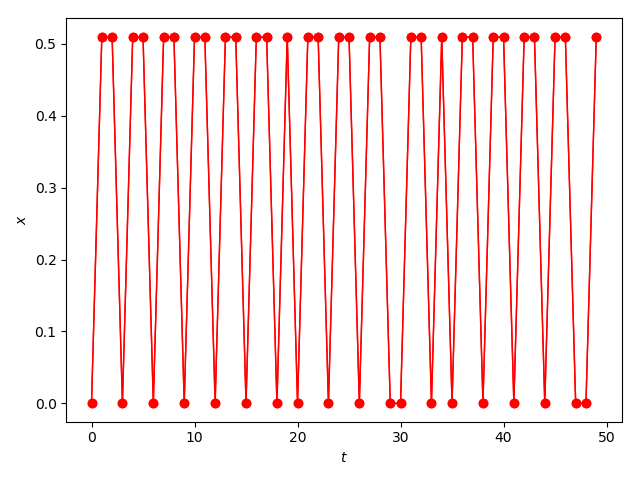
\includegraphics[width=0.5\textwidth]{figures/nbl/inflation-0/sims_x}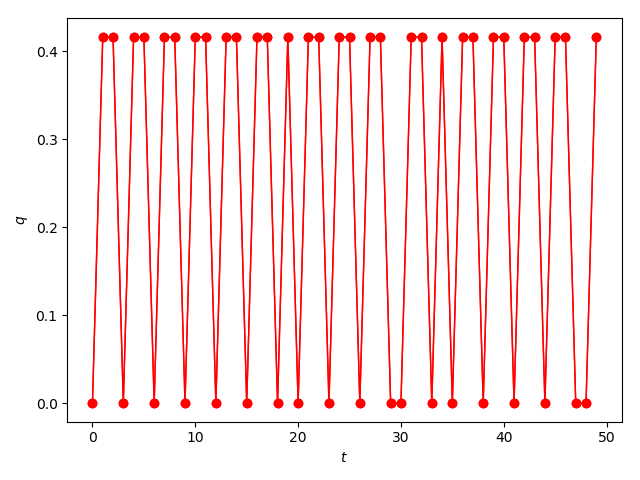
\includegraphics[width=0.5\textwidth]{figures/nbl/inflation-0/sims_q}
\par\end{centering}
\begin{centering}
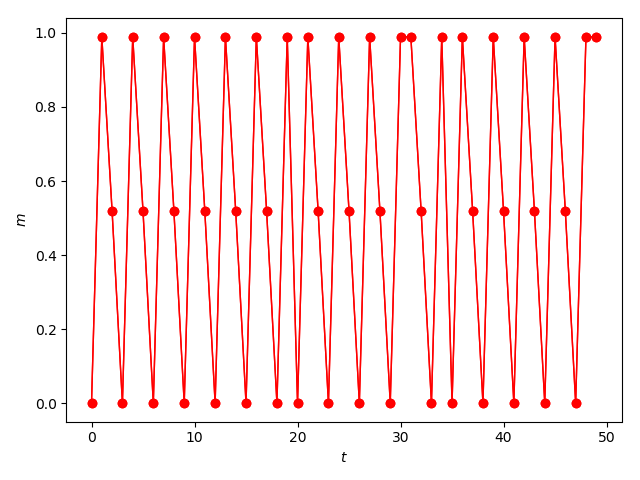
\includegraphics[width=0.5\textwidth]{figures/nbl/inflation-0/sims_m}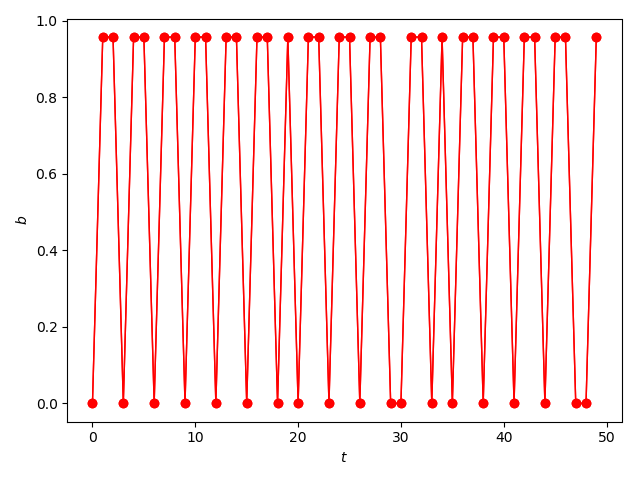
\includegraphics[width=0.5\textwidth]{figures/nbl/inflation-0/sims_b}
\par\end{centering}
\begin{centering}
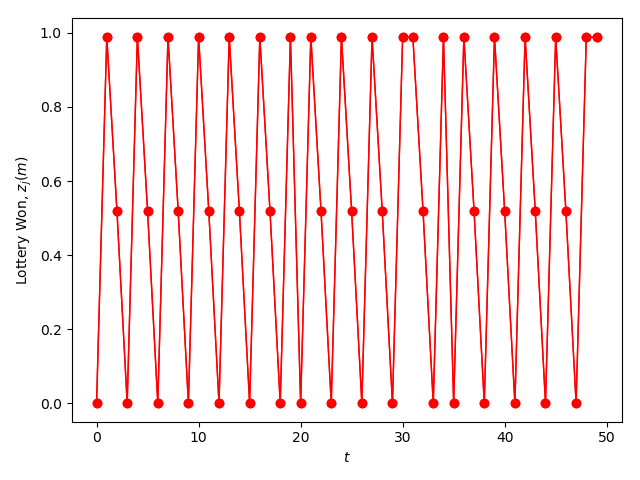
\includegraphics[width=0.5\textwidth]{figures/nbl/inflation-0/sims_lottery}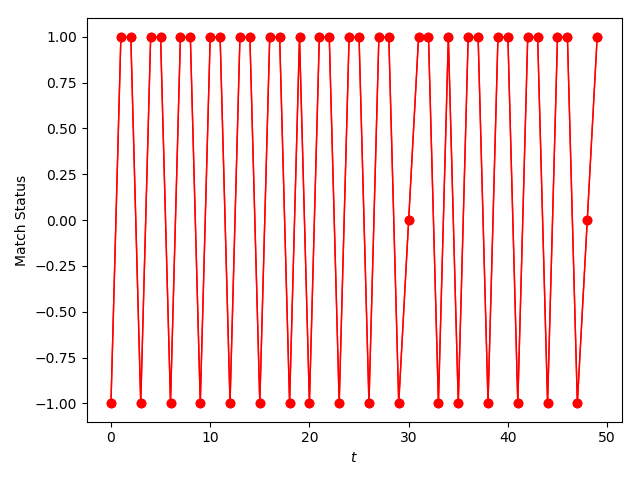
\includegraphics[width=0.5\textwidth]{figures/nbl/inflation-0/sims_match}
\par\end{centering}
\centering{}\caption{\protect\label{fig:Agent-sample-path}Agent sample path (Benchmark
economy). Match Status: $0$ (No Match in DM), $1$ (Match in DM),
$-1$ (in CM).}
\end{figure}

In summary, we can observe the following from our simulation: Agents
can trade more than once in the DM sometimes. This depends on their
lottery outcomes. Agents must also pay a fixed cost to enter the CM
to load up on money balances. Depending on their money balance, they
may sometimes find it worthwhile to borrow against their CM income
to pay the fixed cost of CM entry. Thus, we have an equilibrium Baumol-Tobin
type of money spending cycle in the model. Since agents endogenously
do not have complete consumption insurance, the pattern of consumption
in the DM, $q$ in Figure \ref{fig:Agent-sample-path}, is not completely
smooth.

\section{Inflation and overall distribution of money and prices\protect\label{sec:Inflation-and-overall-distro}}

To illustrate this, we compare just the two stationary-equilibrium
regimes, SME$(\tau=0)$ and SME$(\tau=10)$. In Figures \ref{fig:distro-m=000020and=000020tau}
and \ref{fig:distro-p=000020and=000020tau} below, the distributions'
support contain real money balances at the start of each period $t$.

\begin{figure}[H]
\begin{centering}
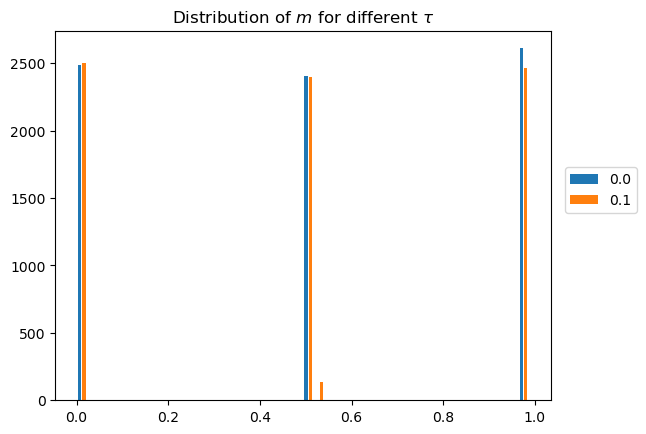
\includegraphics[width=0.5\textwidth]{figures/compare/mechanics/distro-m-inflation}
\par\end{centering}
\caption{Money distribution and inflation for under SME$(\tau=0)$ and SME$(\tau=10)$.\protect\label{fig:distro-m=000020and=000020tau}}
\end{figure}

We observe that intermediate-level money holders spread out in their
masses in Figure \ref{fig:distro-m=000020and=000020tau} as inflation
goes from 0\% (blue/darker bars) to 10\% (orange/lighter bars) \emph{per
annum}. This explains the additional masses in the intermediate region
of the money distribution support. The measure of the highest-balance
agents go down with inflation as agents work less. Additional lotteries
can arise as agents in DM expect to trade faster. There is less mass
in the intermediate $m$ levels as agents trade faster out of the
DM, and for agents who choose to enter the CM, the additional lottery
outcomes push them toward the extreme edges of the high/low prize
outcomes. This observation is associated with the extensive margin
effect so that with higher inflation, there can be a higher inequality
in $m$-wealth distribution.\lyxdeleted{Obiwan Kenobi}{Mon Apr  7 00:52:33 2025}{�}

At 0\% inflation, despite the possibility of different submarkets
in the DM, it turns out that there is no price dispersion. However,
at 10\% inflation, there is a marked distribution of pricing outcomes.

\begin{figure}[H]
\begin{centering}
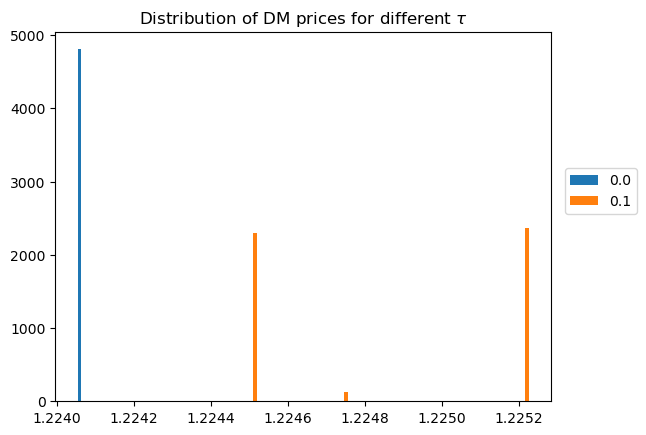
\includegraphics[width=0.55\textwidth]{figures/compare/mechanics/distro-p-inflation}
\par\end{centering}
\caption{DM (submarkets) pricing function ($p$) and inflation. Distribution
of DM pricing outcomes $p(m)$ for under SME$(\tau=0)$ and SME$(\tau=10)$.
\protect\label{fig:distro-p=000020and=000020tau}}
\end{figure}

\end{document}
